\documentclass[twoside]{book}

% Packages required by doxygen
\usepackage{fixltx2e}
\usepackage{calc}
\usepackage{doxygen}
\usepackage[export]{adjustbox} % also loads graphicx
\usepackage{graphicx}
\usepackage[utf8]{inputenc}
\usepackage{makeidx}
\usepackage{multicol}
\usepackage{multirow}
\PassOptionsToPackage{warn}{textcomp}
\usepackage{textcomp}
\usepackage[nointegrals]{wasysym}
\usepackage[table]{xcolor}

% Font selection
\usepackage[T1]{fontenc}
\usepackage[scaled=.90]{helvet}
\usepackage{courier}
\usepackage{amssymb}
\usepackage{sectsty}
\renewcommand{\familydefault}{\sfdefault}
\allsectionsfont{%
  \fontseries{bc}\selectfont%
  \color{darkgray}%
}
\renewcommand{\DoxyLabelFont}{%
  \fontseries{bc}\selectfont%
  \color{darkgray}%
}
\newcommand{\+}{\discretionary{\mbox{\scriptsize$\hookleftarrow$}}{}{}}

% Page & text layout
\usepackage{geometry}
\geometry{%
  a4paper,%
  top=2.5cm,%
  bottom=2.5cm,%
  left=2.5cm,%
  right=2.5cm%
}
\tolerance=750
\hfuzz=15pt
\hbadness=750
\setlength{\emergencystretch}{15pt}
\setlength{\parindent}{0cm}
\setlength{\parskip}{3ex plus 2ex minus 2ex}
\makeatletter
\renewcommand{\paragraph}{%
  \@startsection{paragraph}{4}{0ex}{-1.0ex}{1.0ex}{%
    \normalfont\normalsize\bfseries\SS@parafont%
  }%
}
\renewcommand{\subparagraph}{%
  \@startsection{subparagraph}{5}{0ex}{-1.0ex}{1.0ex}{%
    \normalfont\normalsize\bfseries\SS@subparafont%
  }%
}
\makeatother

% Headers & footers
\usepackage{fancyhdr}
\pagestyle{fancyplain}
\fancyhead[LE]{\fancyplain{}{\bfseries\thepage}}
\fancyhead[CE]{\fancyplain{}{}}
\fancyhead[RE]{\fancyplain{}{\bfseries\leftmark}}
\fancyhead[LO]{\fancyplain{}{\bfseries\rightmark}}
\fancyhead[CO]{\fancyplain{}{}}
\fancyhead[RO]{\fancyplain{}{\bfseries\thepage}}
\fancyfoot[LE]{\fancyplain{}{}}
\fancyfoot[CE]{\fancyplain{}{}}
\fancyfoot[RE]{\fancyplain{}{\bfseries\scriptsize Generated by Doxygen }}
\fancyfoot[LO]{\fancyplain{}{\bfseries\scriptsize Generated by Doxygen }}
\fancyfoot[CO]{\fancyplain{}{}}
\fancyfoot[RO]{\fancyplain{}{}}
\renewcommand{\footrulewidth}{0.4pt}
\renewcommand{\chaptermark}[1]{%
  \markboth{#1}{}%
}
\renewcommand{\sectionmark}[1]{%
  \markright{\thesection\ #1}%
}

% Indices & bibliography
\usepackage{natbib}
\usepackage[titles]{tocloft}
\setcounter{tocdepth}{3}
\setcounter{secnumdepth}{5}
\makeindex

% Hyperlinks (required, but should be loaded last)
\usepackage{ifpdf}
\ifpdf
  \usepackage[pdftex,pagebackref=true]{hyperref}
\else
  \usepackage[ps2pdf,pagebackref=true]{hyperref}
\fi
\hypersetup{%
  colorlinks=true,%
  linkcolor=blue,%
  citecolor=blue,%
  unicode%
}

% Custom commands
\newcommand{\clearemptydoublepage}{%
  \newpage{\pagestyle{empty}\cleardoublepage}%
}

\usepackage{caption}
\captionsetup{labelsep=space,justification=centering,font={bf},singlelinecheck=off,skip=4pt,position=top}

%===== C O N T E N T S =====

\begin{document}

% Titlepage & ToC
\hypersetup{pageanchor=false,
             bookmarksnumbered=true,
             pdfencoding=unicode
            }
\pagenumbering{roman}
\begin{titlepage}
\vspace*{7cm}
\begin{center}%
{\Large My Project }\\
\vspace*{1cm}
{\large Generated by Doxygen 1.8.11}\\
\end{center}
\end{titlepage}
\clearemptydoublepage
\tableofcontents
\clearemptydoublepage
\pagenumbering{arabic}
\hypersetup{pageanchor=true}

%--- Begin generated contents ---
\chapter{File Index}
\section{File List}
Here is a list of all documented files with brief descriptions\-:\begin{DoxyCompactList}
\item\contentsline{section}{\hyperlink{BGField1_8hh}{B\-G\-Field1.\-hh} \\*B\-G\-Field1-\/7 are 7 almost identical headers that define 7 similar classes derived from \char`\"{}\-E\-M\-M\-A\-Element\-Field.\-hh.\char`\"{} They each descibe an E\-M field that is part of E\-M\-M\-A }{\pageref{BGField1_8hh}}{}
\item\contentsline{section}{\hyperlink{BGField2_8hh}{B\-G\-Field2.\-hh} \\*B\-G\-Field1-\/7 are 7 almost identical headers that define 7 similar classes derived from \char`\"{}\-E\-M\-M\-A\-Element\-Field.\-hh.\char`\"{} They each descibe an E\-M field that is part of E\-M\-M\-A }{\pageref{BGField2_8hh}}{}
\item\contentsline{section}{\hyperlink{BGField3_8hh}{B\-G\-Field3.\-hh} \\*B\-G\-Field1-\/7 are 7 almost identical headers that define 7 similar classes derived from \char`\"{}\-E\-M\-M\-A\-Element\-Field.\-hh.\char`\"{} They each descibe an E\-M field that is part of E\-M\-M\-A }{\pageref{BGField3_8hh}}{}
\item\contentsline{section}{\hyperlink{BGField4_8hh}{B\-G\-Field4.\-hh} \\*B\-G\-Field1-\/7 are 7 almost identical headers that define 7 similar classes derived from \char`\"{}\-E\-M\-M\-A\-Element\-Field.\-hh.\char`\"{} They each descibe an E\-M field that is part of E\-M\-M\-A }{\pageref{BGField4_8hh}}{}
\item\contentsline{section}{\hyperlink{BGField5_8hh}{B\-G\-Field5.\-hh} \\*B\-G\-Field1-\/7 are 7 almost identical headers that define 7 similar classes derived from \char`\"{}\-E\-M\-M\-A\-Element\-Field.\-hh.\char`\"{} They each descibe an E\-M field that is part of E\-M\-M\-A }{\pageref{BGField5_8hh}}{}
\item\contentsline{section}{\hyperlink{BGField6_8hh}{B\-G\-Field6.\-hh} \\*B\-G\-Field1-\/7 are 7 almost identical headers that define 7 similar classes derived from \char`\"{}\-E\-M\-M\-A\-Element\-Field.\-hh.\char`\"{} They each descibe an E\-M field that is part of E\-M\-M\-A }{\pageref{BGField6_8hh}}{}
\item\contentsline{section}{\hyperlink{BGField7_8hh}{B\-G\-Field7.\-hh} \\*B\-G\-Field1-\/7 are 7 almost identical headers that define 7 similar classes derived from \char`\"{}\-E\-M\-M\-A\-Element\-Field.\-hh.\char`\"{} They each descibe an E\-M field that is part of E\-M\-M\-A }{\pageref{BGField7_8hh}}{}
\item\contentsline{section}{\hyperlink{c2__factory_8hh}{c2\-\_\-factory.\-hh} \\*Provides a factory class to avoid an infinite number of template declarations }{\pageref{c2__factory_8hh}}{}
\item\contentsline{section}{\hyperlink{c2__function_8hh}{c2\-\_\-function.\-hh} \\*Provides the headers for the general \hyperlink{classc2__function}{c2\-\_\-function} algebra which supports fast, flexible operations on piecewise-\/twice-\/differentiable functions }{\pageref{c2__function_8hh}}{}
\item\contentsline{section}{\hyperlink{CathodeWireParameterisation_8hh}{Cathode\-Wire\-Parameterisation.\-hh} \\*This is a parameterisation that describes a series of cylinders (wires) along X }{\pageref{CathodeWireParameterisation_8hh}}{}
\item\contentsline{section}{\hyperlink{EMFieldDebugger_8hh}{E\-M\-Field\-Debugger.\-hh} \\*This header declares a class used in the corresponding source file that calculates the value of E\-M fields at different locations in the simulation }{\pageref{EMFieldDebugger_8hh}}{}
\item\contentsline{section}{\hyperlink{EMMAAnalysisManager_8hh}{E\-M\-M\-A\-Analysis\-Manager.\-hh} \\*This header calls upon several root files and declares other functions for a source file. These functions call upon and write to R\-O\-O\-T files to display simulation outcomes or results }{\pageref{EMMAAnalysisManager_8hh}}{}
\item\contentsline{section}{\hyperlink{EMMADetectorConstMessenger_8hh}{E\-M\-M\-A\-Detector\-Const\-Messenger.\-hh} \\*This header file contains deals with user commands relating to detector construction }{\pageref{EMMADetectorConstMessenger_8hh}}{}
\item\contentsline{section}{\hyperlink{EMMADetectorConstruction_8hh}{E\-M\-M\-A\-Detector\-Construction.\-hh} \\*This header file builds on the G4 header \char`\"{}\-G4\-V\-User\-Detector\-Construction.\-hh\char`\"{} to set the global G4 variables specifying the materials and simulation attributes of the E\-M\-M\-A detectors. Several E\-M\-M\-A functions (regarding its detectors) are also defined }{\pageref{EMMADetectorConstruction_8hh}}{}
\item\contentsline{section}{\hyperlink{EMMADriftChamber_8hh}{E\-M\-M\-A\-Drift\-Chamber.\-hh} \\*This header contains the class required to run the P\-G\-A\-C drift chamber (see also G4\-Sensitive\-Detector.\-hh) }{\pageref{EMMADriftChamber_8hh}}{}
\item\contentsline{section}{\hyperlink{EMMADriftChamberHit_8hh}{E\-M\-M\-A\-Drift\-Chamber\-Hit.\-hh} \\*This class manages the hit object in regards to the drift chamber part of the simulation. It defines global variables and functions for the G4 code to run necessary hit simulations. The virtual methods draw() and print() are used. For further details about each part of this file, examine the accompanying explanations adjacent to the classes }{\pageref{EMMADriftChamberHit_8hh}}{}
\item\contentsline{section}{\hyperlink{EMMAElementField_8hh}{E\-M\-M\-A\-Element\-Field.\-hh} \\*This is the interface class used by Global\-Field to compute the field value at a given point\mbox{[}\mbox{]} }{\pageref{EMMAElementField_8hh}}{}
\item\contentsline{section}{\hyperlink{EMMAEMPhysics_8hh}{E\-M\-M\-A\-E\-M\-Physics.\-hh} \\*The G4 header \char`\"{}\-G4\-V\-Physics\-Constructor.\-hh\char`\"{} contains a virtual class that must be used to create concrete classes for specific applications (such as E\-M\-M\-A). This header builds such a concrete class to include E\-M\-M\-A's specific particles and processes. Specifically, this header defines particles and processes required to simulate E\-M interactions }{\pageref{EMMAEMPhysics_8hh}}{}
\item\contentsline{section}{\hyperlink{EMMAEventAction_8hh}{E\-M\-M\-A\-Event\-Action.\-hh} \\*This header defines the user's action class, and specifically, the beginning and end of a user action. It generates from the Primary\-Generator headers as the user begins an action. Contains functions that are invoked by G4\-Event\-Manager }{\pageref{EMMAEventAction_8hh}}{}
\item\contentsline{section}{\hyperlink{EMMAEventActionMessenger_8hh}{E\-M\-M\-A\-Event\-Action\-Messenger.\-hh} \\*This file is responsible for deleting commands, delivering commands to destination classes, defining global G4 variables specific to E\-M\-M\-A, and replying the current values of the parameters (again as described the \char`\"{}\-G4\-U\-Imessenger.\-hh\char`\"{} source file) regarding the event action (from the primary generator) }{\pageref{EMMAEventActionMessenger_8hh}}{}
\item\contentsline{section}{\hyperlink{EMMAGeneralPhysics_8hh}{E\-M\-M\-A\-General\-Physics.\-hh} \\*This header defines particles and processes required for other more specific physics processes }{\pageref{EMMAGeneralPhysics_8hh}}{}
\item\contentsline{section}{\hyperlink{EMMAGlobalField_8hh}{E\-M\-M\-A\-Global\-Field.\-hh} \\*Handles the global Electro\-Magnetic field }{\pageref{EMMAGlobalField_8hh}}{}
\item\contentsline{section}{\hyperlink{EMMAHadronPhysics_8hh}{E\-M\-M\-A\-Hadron\-Physics.\-hh} \\*The G4 header \char`\"{}\-G4\-V\-Physics\-Constructor.\-hh\char`\"{} contains a virtual class that must be used to create concrete classes for specific applications (such as E\-M\-M\-A). Specifically, this header defines particles and processes required to simulate hadron interactions }{\pageref{EMMAHadronPhysics_8hh}}{}
\item\contentsline{section}{\hyperlink{EMMAIonChamber_8hh}{E\-M\-M\-A\-Ion\-Chamber.\-hh} \\*This defines a calorimeter sensitive detector class (ion chamber). Uses the inherited G4 detector construction classes to build the operation of the ion chamber }{\pageref{EMMAIonChamber_8hh}}{}
\item\contentsline{section}{\hyperlink{EMMAIonChamberHit_8hh}{E\-M\-M\-A\-Ion\-Chamber\-Hit.\-hh} \\*Calorimeter (ion chamber) hit class\-: defines data members to store the the energy deposit and track lengths of charged particles in a selected volume }{\pageref{EMMAIonChamberHit_8hh}}{}
\item\contentsline{section}{\hyperlink{EMMAIonPhysics_8hh}{E\-M\-M\-A\-Ion\-Physics.\-hh} \\*The G4 header \char`\"{}\-G4\-V\-Physics\-Constructor.\-hh\char`\"{} contains a virtual class that must be used to create concrete classes for specific applications (such as E\-M\-M\-A). Specifically, this header defines particles and processes required to simulate ion interactions }{\pageref{EMMAIonPhysics_8hh}}{}
\item\contentsline{section}{\hyperlink{EMMAIonPhysicsMessenger_8hh}{E\-M\-M\-A\-Ion\-Physics\-Messenger.\-hh} \\*This header file contains deals with user commands relating to ionic physics processes }{\pageref{EMMAIonPhysicsMessenger_8hh}}{}
\item\contentsline{section}{\hyperlink{EMMAMuonPhysics_8hh}{E\-M\-M\-A\-Muon\-Physics.\-hh} \\*The G4 header \char`\"{}\-G4\-V\-Physics\-Constructor.\-hh\char`\"{} contains a virtual class that must be used to create concrete classes for specific applications (such as E\-M\-M\-A). Specifically, this header defines particles and processes required to simulate muon interactions }{\pageref{EMMAMuonPhysics_8hh}}{}
\item\contentsline{section}{\hyperlink{EMMANuclearReactionDataSet_8hh}{E\-M\-M\-A\-Nuclear\-Reaction\-Data\-Set.\-hh} \\*Data set for (two body) nuclear reaction cross sections. Inherited from similar G4 headers }{\pageref{EMMANuclearReactionDataSet_8hh}}{}
\item\contentsline{section}{\hyperlink{EMMANuclearReactionProcess_8hh}{E\-M\-M\-A\-Nuclear\-Reaction\-Process.\-hh} \\*Nuclear-\/reaction process for projectile (Z1,A1) striking target (Z2,A2) with cross section (cs) }{\pageref{EMMANuclearReactionProcess_8hh}}{}
\item\contentsline{section}{\hyperlink{EMMANuclearReactionTwoBody_8hh}{E\-M\-M\-A\-Nuclear\-Reaction\-Two\-Body.\-hh} \\*Nuclear-\/reaction model for two-\/body final-\/state (Z3,A3)+(Z4,A4) after a two body reaction between a projectile and target }{\pageref{EMMANuclearReactionTwoBody_8hh}}{}
\item\contentsline{section}{\hyperlink{EMMAPhysicsList_8hh}{E\-M\-M\-A\-Physics\-List.\-hh} \\*E\-M\-M\-A's specific objects and particles are registered from the virtual class in \char`\"{}\-G4\-V\-Physics\-Constructor.\-hh.\char`\"{} These objects are registered to G4\-User\-Physics\-List, which is the parent of \char`\"{}\-G4\-V\-Modular\-Physics\-List.\-hh.\char`\"{} This header defines a concrete class inherited from \char`\"{}\-G4\-V\-Modular\-Physics\-List.\-hh\char`\"{} }{\pageref{EMMAPhysicsList_8hh}}{}
\item\contentsline{section}{\hyperlink{EMMAPrimaryGeneratorAction_8hh}{E\-M\-M\-A\-Primary\-Generator\-Action.\-hh} \\*This is an important class responsible for primary particle or vertex generation. It is required by G4; the Primary Generator is not an actual physical component of E\-M\-M\-A but rather a G4 construction element. This class is the concrete class stemming from the virtual class found in \char`\"{}\-G4\-V\-User\-Primary\-Generator\-Action.\-hh.\char`\"{} }{\pageref{EMMAPrimaryGeneratorAction_8hh}}{}
\item\contentsline{section}{\hyperlink{EMMAPrimaryGeneratorMessenger_8hh}{E\-M\-M\-A\-Primary\-Generator\-Messenger.\-hh} \\*This file is responsible for deleting commands, delivering commands to destination classes, defining global G4 variables specific to E\-M\-M\-A, and replying the current values of the parameters (again as described the \char`\"{}\-G4\-U\-Imessenger.\-hh\char`\"{} source file) regarding the primary generator (of the events) }{\pageref{EMMAPrimaryGeneratorMessenger_8hh}}{}
\item\contentsline{section}{\hyperlink{EMMASteppingAction_8hh}{E\-M\-M\-A\-Stepping\-Action.\-hh} \\*Headers that have to do with \char`\"{}stepping\char`\"{} (loops) is related to tracking the particle and its interactions with its surroundings. This class defines functions that build on \char`\"{}\-G4\-User\-Stepping\-Action.\-hh,\char`\"{} which represents user actions during \char`\"{}stepping.\char`\"{} }{\pageref{EMMASteppingAction_8hh}}{}
\item\contentsline{section}{\hyperlink{EMMASteppingVerbose_8hh}{E\-M\-M\-A\-Stepping\-Verbose.\-hh} \\*This class manages the verbose outputs in G4\-Stepping\-Manager. It shows how to extract information during the tracking of a particle }{\pageref{EMMASteppingVerbose_8hh}}{}
\item\contentsline{section}{\hyperlink{F04StepMax_8hh}{F04\-Step\-Max.\-hh} \\*Header defines a class relating to the step (tracking) of a particle involved in a discrete process. For more general information see this header's dependencies }{\pageref{F04StepMax_8hh}}{}
\item\contentsline{section}{\hyperlink{G4LindhardPartition_8hh}{G4\-Lindhard\-Partition.\-hh} \\*A seemingly periphery code that calculates the non-\/ionizing energy loss of radiation via the Lindhard partition function. Used to calculate energy deposited in target by the beam thereby affecting energy of recoils }{\pageref{G4LindhardPartition_8hh}}{}
\item\contentsline{section}{\hyperlink{G4ScreenedNuclearRecoil_8hh}{G4\-Screened\-Nuclear\-Recoil.\-hh} \\*Builds the process of screened electromagnetic nuclear elastic scattering. Declares many functions primarily used for coulomb interactions between nuclei }{\pageref{G4ScreenedNuclearRecoil_8hh}}{}
\item\contentsline{section}{\hyperlink{PGACWireParameterisation_8hh}{P\-G\-A\-C\-Wire\-Parameterisation.\-hh} \\*A parameterisation that describes a series of cylinders along Z (the wires in the P\-C\-A\-G ioin drift chamber) }{\pageref{PGACWireParameterisation_8hh}}{}
\item\contentsline{section}{\hyperlink{SpectrometerConstruction_8hh}{Spectrometer\-Construction.\-hh} \\*Builds the E\-M\-M\-A spectrometer through defining classes and variables, including those for slit control. This header is built upon the virtual classes inherited from \char`\"{}\-G4\-V\-User\-Detector\-Construction.\-hh.\char`\"{} }{\pageref{SpectrometerConstruction_8hh}}{}
\item\contentsline{section}{{\bfseries Stacking\-Action.\-hh} }{\pageref{StackingAction_8hh}}{}
\item\contentsline{section}{{\bfseries Tracking\-Action.\-hh} }{\pageref{TrackingAction_8hh}}{}
\end{DoxyCompactList}

\chapter{File Documentation}
\hypertarget{BGField1_8cc}{\section{B\-G\-Field1.\-cc File Reference}
\label{BGField1_8cc}\index{B\-G\-Field1.\-cc@{B\-G\-Field1.\-cc}}
}


The B\-G\-Field source files construct the 7 magnetic and electric fields on the E\-M\-M\-A simulation (Q\-Q\-E\-M\-E\-Q\-Q).  


{\ttfamily \#include \char`\"{}B\-G\-Field1.\-hh\char`\"{}}\\*
{\ttfamily \#include \char`\"{}fortran\-\_\-subs.\-inc\char`\"{}}\\*
{\ttfamily \#include \char`\"{}G4ios.\-hh\char`\"{}}\\*
{\ttfamily \#include \char`\"{}G4\-Units\-Table.\-hh\char`\"{}}\\*
{\ttfamily \#include $<$fstream$>$}\\*
{\ttfamily \#include \char`\"{}E\-M\-M\-A\-Element\-Field.\-hh\char`\"{}}\\*


\subsection{Detailed Description}
The B\-G\-Field source files construct the 7 magnetic and electric fields on the E\-M\-M\-A simulation (Q\-Q\-E\-M\-E\-Q\-Q). 
\hypertarget{BGField2_8cc}{}\section{B\+G\+Field2.\+cc File Reference}
\label{BGField2_8cc}\index{B\+G\+Field2.\+cc@{B\+G\+Field2.\+cc}}
{\ttfamily \#include \char`\"{}B\+G\+Field2.\+hh\char`\"{}}\\*
{\ttfamily \#include \char`\"{}fortran\+\_\+subs.\+inc\char`\"{}}\\*
{\ttfamily \#include \char`\"{}G4\+Units\+Table.\+hh\char`\"{}}\\*
{\ttfamily \#include $<$fstream$>$}\\*
{\ttfamily \#include \char`\"{}E\+M\+M\+A\+Global\+Field.\+hh\char`\"{}}\\*
Include dependency graph for B\+G\+Field2.\+cc\+:
\nopagebreak
\begin{figure}[H]
\begin{center}
\leavevmode
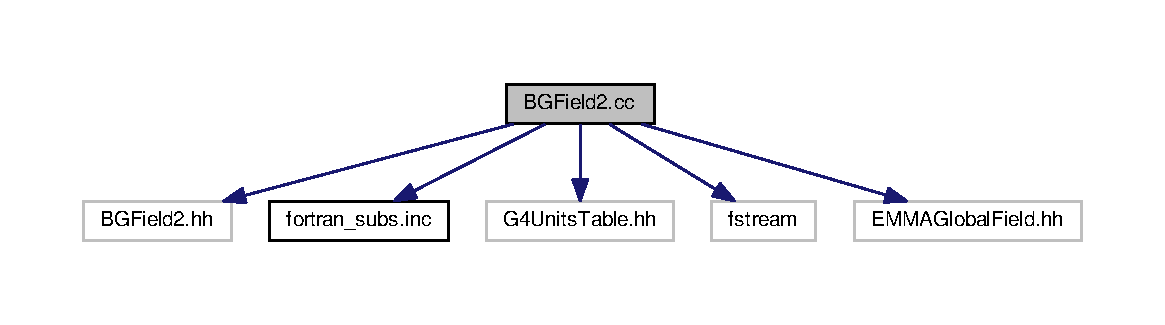
\includegraphics[width=350pt]{BGField2_8cc__incl}
\end{center}
\end{figure}

\hypertarget{BGField3_8cc}{}\section{B\+G\+Field3.\+cc File Reference}
\label{BGField3_8cc}\index{B\+G\+Field3.\+cc@{B\+G\+Field3.\+cc}}
{\ttfamily \#include \char`\"{}B\+G\+Field3.\+hh\char`\"{}}\\*
{\ttfamily \#include \char`\"{}fortran\+\_\+subs.\+inc\char`\"{}}\\*
{\ttfamily \#include \char`\"{}G4\+Units\+Table.\+hh\char`\"{}}\\*
{\ttfamily \#include $<$fstream$>$}\\*
{\ttfamily \#include \char`\"{}E\+M\+M\+A\+Global\+Field.\+hh\char`\"{}}\\*
Include dependency graph for B\+G\+Field3.\+cc\+:
\nopagebreak
\begin{figure}[H]
\begin{center}
\leavevmode
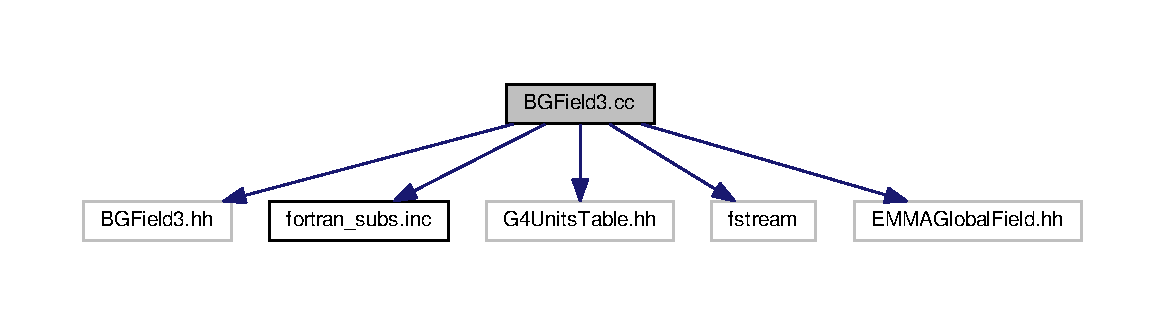
\includegraphics[width=350pt]{BGField3_8cc__incl}
\end{center}
\end{figure}

\hypertarget{BGField4_8cc}{\section{B\-G\-Field4.\-cc File Reference}
\label{BGField4_8cc}\index{B\-G\-Field4.\-cc@{B\-G\-Field4.\-cc}}
}


The B\-G\-Field source files construct the 7 magnetic and electric fields on the E\-M\-M\-A simulation (Q\-Q\-E\-M\-E\-Q\-Q).  


{\ttfamily \#include \char`\"{}B\-G\-Field4.\-hh\char`\"{}}\\*
{\ttfamily \#include \char`\"{}fortran\-\_\-subs.\-inc\char`\"{}}\\*
{\ttfamily \#include \char`\"{}G4\-Units\-Table.\-hh\char`\"{}}\\*
{\ttfamily \#include \char`\"{}E\-M\-M\-A\-Global\-Field.\-hh\char`\"{}}\\*
{\ttfamily \#include $<$fstream$>$}\\*


\subsection{Detailed Description}
The B\-G\-Field source files construct the 7 magnetic and electric fields on the E\-M\-M\-A simulation (Q\-Q\-E\-M\-E\-Q\-Q). 
\hypertarget{BGField5_8cc}{\section{B\-G\-Field5.\-cc File Reference}
\label{BGField5_8cc}\index{B\-G\-Field5.\-cc@{B\-G\-Field5.\-cc}}
}


The B\-G\-Field source files construct the 7 magnetic and electric fields on the E\-M\-M\-A simulation (Q\-Q\-E\-M\-E\-Q\-Q).  


{\ttfamily \#include \char`\"{}B\-G\-Field5.\-hh\char`\"{}}\\*
{\ttfamily \#include \char`\"{}fortran\-\_\-subs.\-inc\char`\"{}}\\*
{\ttfamily \#include \char`\"{}G4\-Units\-Table.\-hh\char`\"{}}\\*
{\ttfamily \#include $<$fstream$>$}\\*
{\ttfamily \#include \char`\"{}E\-M\-M\-A\-Global\-Field.\-hh\char`\"{}}\\*


\subsection{Detailed Description}
The B\-G\-Field source files construct the 7 magnetic and electric fields on the E\-M\-M\-A simulation (Q\-Q\-E\-M\-E\-Q\-Q). 
\hypertarget{BGField6_8cc}{}\section{B\+G\+Field6.\+cc File Reference}
\label{BGField6_8cc}\index{B\+G\+Field6.\+cc@{B\+G\+Field6.\+cc}}
{\ttfamily \#include \char`\"{}B\+G\+Field6.\+hh\char`\"{}}\\*
{\ttfamily \#include \char`\"{}fortran\+\_\+subs.\+inc\char`\"{}}\\*
{\ttfamily \#include \char`\"{}G4\+Units\+Table.\+hh\char`\"{}}\\*
{\ttfamily \#include $<$fstream$>$}\\*
{\ttfamily \#include \char`\"{}E\+M\+M\+A\+Global\+Field.\+hh\char`\"{}}\\*
Include dependency graph for B\+G\+Field6.\+cc\+:
\nopagebreak
\begin{figure}[H]
\begin{center}
\leavevmode
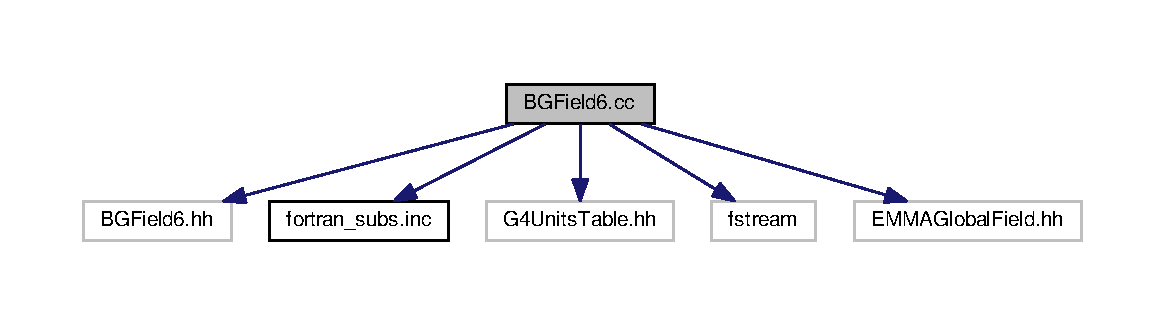
\includegraphics[width=350pt]{BGField6_8cc__incl}
\end{center}
\end{figure}

\hypertarget{BGField7_8cc}{}\section{B\+G\+Field7.\+cc File Reference}
\label{BGField7_8cc}\index{B\+G\+Field7.\+cc@{B\+G\+Field7.\+cc}}
{\ttfamily \#include \char`\"{}B\+G\+Field7.\+hh\char`\"{}}\\*
{\ttfamily \#include \char`\"{}fortran\+\_\+subs.\+inc\char`\"{}}\\*
{\ttfamily \#include \char`\"{}G4\+Units\+Table.\+hh\char`\"{}}\\*
{\ttfamily \#include $<$fstream$>$}\\*
{\ttfamily \#include \char`\"{}E\+M\+M\+A\+Global\+Field.\+hh\char`\"{}}\\*
Include dependency graph for B\+G\+Field7.\+cc\+:
\nopagebreak
\begin{figure}[H]
\begin{center}
\leavevmode
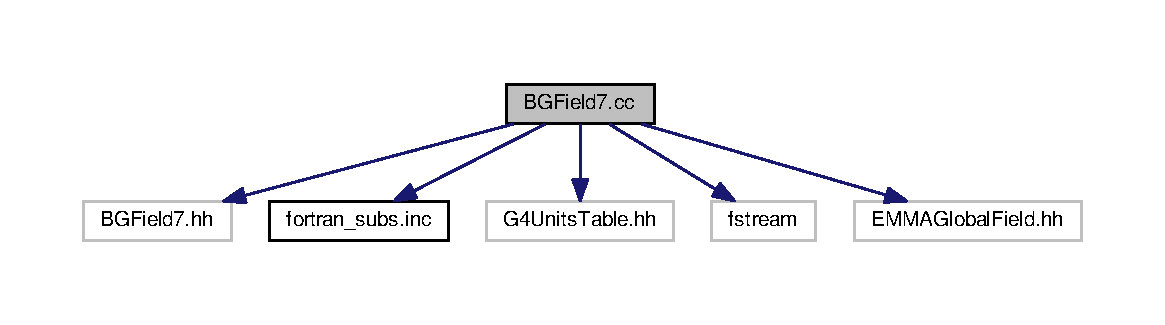
\includegraphics[width=350pt]{BGField7_8cc__incl}
\end{center}
\end{figure}

\hypertarget{EMFieldDebugger_8cc}{}\section{E\+M\+Field\+Debugger.\+cc File Reference}
\label{EMFieldDebugger_8cc}\index{E\+M\+Field\+Debugger.\+cc@{E\+M\+Field\+Debugger.\+cc}}
{\ttfamily \#include \char`\"{}E\+M\+Field\+Debugger.\+hh\char`\"{}}\\*
{\ttfamily \#include \char`\"{}E\+M\+M\+A\+Global\+Field.\+hh\char`\"{}}\\*
{\ttfamily \#include \char`\"{}G4\+Units\+Table.\+hh\char`\"{}}\\*
{\ttfamily \#include $<$iomanip$>$}\\*
{\ttfamily \#include $<$fstream$>$}\\*
{\ttfamily \#include $<$stdlib.\+h$>$}\\*
{\ttfamily \#include \char`\"{}G4\+System\+Of\+Units.\+hh\char`\"{}}\\*
Include dependency graph for E\+M\+Field\+Debugger.\+cc\+:
\nopagebreak
\begin{figure}[H]
\begin{center}
\leavevmode
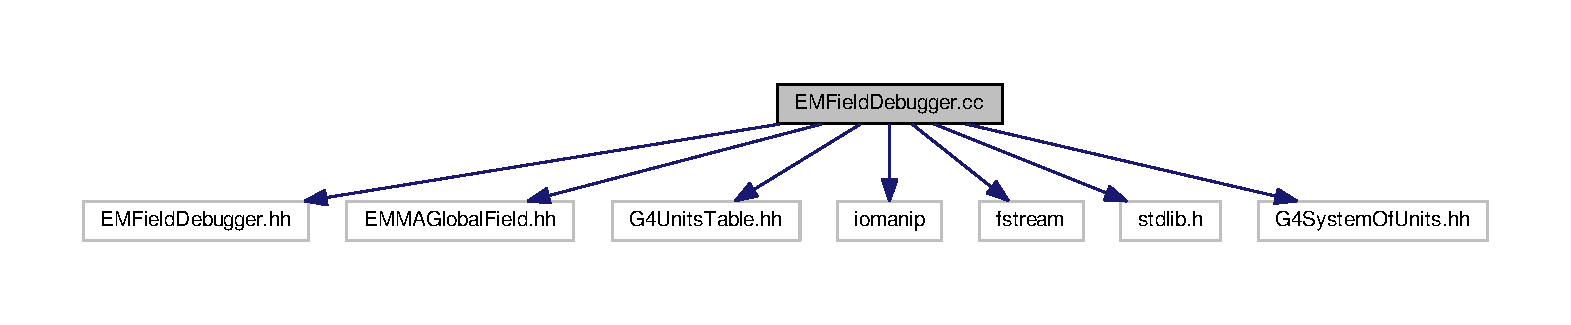
\includegraphics[width=350pt]{EMFieldDebugger_8cc__incl}
\end{center}
\end{figure}

\hypertarget{EMMAAnalysisManager_8cc}{\section{E\-M\-M\-A\-Analysis\-Manager.\-cc File Reference}
\label{EMMAAnalysisManager_8cc}\index{E\-M\-M\-A\-Analysis\-Manager.\-cc@{E\-M\-M\-A\-Analysis\-Manager.\-cc}}
}


Calls upon and writes to R\-O\-O\-T files to display results and outcomes.  




\subsection{Detailed Description}
Calls upon and writes to R\-O\-O\-T files to display results and outcomes. 
\hypertarget{EMMADetectorConstMessenger_8cc}{\section{E\-M\-M\-A\-Detector\-Const\-Messenger.\-cc File Reference}
\label{EMMADetectorConstMessenger_8cc}\index{E\-M\-M\-A\-Detector\-Const\-Messenger.\-cc@{E\-M\-M\-A\-Detector\-Const\-Messenger.\-cc}}
}


Connects U\-I and user input to the detector construction. Takes and gives use commands to/from the user when constructing detectors (the P\-G\-A\-C, the degraders, etc.).  


{\ttfamily \#include \char`\"{}E\-M\-M\-A\-Detector\-Const\-Messenger.\-hh\char`\"{}}\\*
{\ttfamily \#include \char`\"{}E\-M\-M\-A\-Detector\-Construction.\-hh\char`\"{}}\\*
{\ttfamily \#include \char`\"{}G4\-U\-Idirectory.\-hh\char`\"{}}\\*
{\ttfamily \#include \char`\"{}G4\-U\-Icmd\-With\-A\-Double\-And\-Unit.\-hh\char`\"{}}\\*
{\ttfamily \#include \char`\"{}G4\-U\-Icmd\-With\-A\-Double.\-hh\char`\"{}}\\*
{\ttfamily \#include \char`\"{}G4\-U\-Icmd\-Without\-Parameter.\-hh\char`\"{}}\\*
{\ttfamily \#include \char`\"{}G4ios.\-hh\char`\"{}}\\*


\subsection{Detailed Description}
Connects U\-I and user input to the detector construction. Takes and gives use commands to/from the user when constructing detectors (the P\-G\-A\-C, the degraders, etc.). 
\hypertarget{EMMADetectorConstruction_8cc}{}\section{E\+M\+M\+A\+Detector\+Construction.\+cc File Reference}
\label{EMMADetectorConstruction_8cc}\index{E\+M\+M\+A\+Detector\+Construction.\+cc@{E\+M\+M\+A\+Detector\+Construction.\+cc}}
{\ttfamily \#include \char`\"{}E\+M\+M\+A\+Detector\+Construction.\+hh\char`\"{}}\\*
{\ttfamily \#include \char`\"{}G4\+Field\+Manager.\+hh\char`\"{}}\\*
{\ttfamily \#include \char`\"{}G4\+Transportation\+Manager.\+hh\char`\"{}}\\*
{\ttfamily \#include \char`\"{}G4\+Mag\+\_\+\+Usual\+Eq\+Rhs.\+hh\char`\"{}}\\*
{\ttfamily \#include \char`\"{}G4\+Material.\+hh\char`\"{}}\\*
{\ttfamily \#include \char`\"{}G4\+Element.\+hh\char`\"{}}\\*
{\ttfamily \#include \char`\"{}G4\+Material\+Table.\+hh\char`\"{}}\\*
{\ttfamily \#include \char`\"{}G4\+Nist\+Manager.\+hh\char`\"{}}\\*
{\ttfamily \#include \char`\"{}G4\+V\+Solid.\+hh\char`\"{}}\\*
{\ttfamily \#include \char`\"{}G4\+Union\+Solid.\+hh\char`\"{}}\\*
{\ttfamily \#include \char`\"{}G4\+Box.\+hh\char`\"{}}\\*
{\ttfamily \#include \char`\"{}G4\+Tubs.\+hh\char`\"{}}\\*
{\ttfamily \#include \char`\"{}G4\+Logical\+Volume.\+hh\char`\"{}}\\*
{\ttfamily \#include \char`\"{}G4\+V\+Physical\+Volume.\+hh\char`\"{}}\\*
{\ttfamily \#include \char`\"{}G4\+P\+V\+Placement.\+hh\char`\"{}}\\*
{\ttfamily \#include \char`\"{}G4\+P\+V\+Replica.\+hh\char`\"{}}\\*
{\ttfamily \#include \char`\"{}G4\+P\+V\+Parameterised.\+hh\char`\"{}}\\*
{\ttfamily \#include \char`\"{}G4\+User\+Limits.\+hh\char`\"{}}\\*
{\ttfamily \#include \char`\"{}G4\+Trap.\+hh\char`\"{}}\\*
{\ttfamily \#include \char`\"{}G4\+Transform3\+D.\+hh\char`\"{}}\\*
{\ttfamily \#include \char`\"{}G4\+Region.\+hh\char`\"{}}\\*
{\ttfamily \#include \char`\"{}G4\+Region\+Store.\+hh\char`\"{}}\\*
{\ttfamily \#include \char`\"{}G4\+Units\+Table.\+hh\char`\"{}}\\*
{\ttfamily \#include \char`\"{}G4\+Subtraction\+Solid.\+hh\char`\"{}}\\*
{\ttfamily \#include \char`\"{}G4\+System\+Of\+Units.\+hh\char`\"{}}\\*
{\ttfamily \#include \char`\"{}G4\+S\+D\+Manager.\+hh\char`\"{}}\\*
{\ttfamily \#include \char`\"{}G4\+V\+Sensitive\+Detector.\+hh\char`\"{}}\\*
{\ttfamily \#include \char`\"{}G4\+Run\+Manager.\+hh\char`\"{}}\\*
{\ttfamily \#include \char`\"{}G4\+Vis\+Attributes.\+hh\char`\"{}}\\*
{\ttfamily \#include \char`\"{}G4\+Colour.\+hh\char`\"{}}\\*
{\ttfamily \#include \char`\"{}G4ios.\+hh\char`\"{}}\\*
{\ttfamily \#include \char`\"{}E\+M\+M\+A\+Detector\+Const\+Messenger.\+hh\char`\"{}}\\*
{\ttfamily \#include \char`\"{}E\+M\+M\+A\+Drift\+Chamber.\+hh\char`\"{}}\\*
{\ttfamily \#include \char`\"{}E\+M\+M\+A\+Ion\+Chamber.\+hh\char`\"{}}\\*
{\ttfamily \#include \char`\"{}Spectrometer\+Construction.\+hh\char`\"{}}\\*
{\ttfamily \#include \char`\"{}E\+M\+Field\+Debugger.\+hh\char`\"{}}\\*
{\ttfamily \#include \char`\"{}Cathode\+Wire\+Parameterisation.\+hh\char`\"{}}\\*
{\ttfamily \#include \char`\"{}C\+L\+H\+E\+P/\+Units/\+System\+Of\+Units.\+h\char`\"{}}\\*
{\ttfamily \#include \char`\"{}G4\+Uniform\+Mag\+Field.\+hh\char`\"{}}\\*
{\ttfamily \#include $<$fstream$>$}\\*
{\ttfamily \#include $<$stdlib.\+h$>$}\\*
Include dependency graph for E\+M\+M\+A\+Detector\+Construction.\+cc\+:
\nopagebreak
\begin{figure}[H]
\begin{center}
\leavevmode

\includegraphics[width=350pt]{EMMADetectorConstruction_8cc__incl}
\end{center}
\end{figure}
\subsection*{Variables}
\begin{DoxyCompactItemize}
\item 
G4double \hyperlink{EMMADetectorConstruction_8cc_aeb29decdede3d925164d390a2bf4a67a}{magnetic\+Scaling} = 1
\item 
G4double \hyperlink{EMMADetectorConstruction_8cc_a528ee0b2618db44ed7b0734789834f3d}{electric\+Scaling} = 1
\item 
G4double \hyperlink{EMMADetectorConstruction_8cc_a168924eff042d94e1e59a05bbcdcca38}{target\+Thickness}
\item 
G4double \hyperlink{EMMADetectorConstruction_8cc_a7d65bdf83ece33e0fa248e3da81e825a}{target\+Zoffset}
\end{DoxyCompactItemize}


\subsection{Variable Documentation}
\index{E\+M\+M\+A\+Detector\+Construction.\+cc@{E\+M\+M\+A\+Detector\+Construction.\+cc}!electric\+Scaling@{electric\+Scaling}}
\index{electric\+Scaling@{electric\+Scaling}!E\+M\+M\+A\+Detector\+Construction.\+cc@{E\+M\+M\+A\+Detector\+Construction.\+cc}}
\subsubsection[{\texorpdfstring{electric\+Scaling}{electricScaling}}]{\setlength{\rightskip}{0pt plus 5cm}G4double electric\+Scaling = 1}\hypertarget{EMMADetectorConstruction_8cc_a528ee0b2618db44ed7b0734789834f3d}{}\label{EMMADetectorConstruction_8cc_a528ee0b2618db44ed7b0734789834f3d}
\index{E\+M\+M\+A\+Detector\+Construction.\+cc@{E\+M\+M\+A\+Detector\+Construction.\+cc}!magnetic\+Scaling@{magnetic\+Scaling}}
\index{magnetic\+Scaling@{magnetic\+Scaling}!E\+M\+M\+A\+Detector\+Construction.\+cc@{E\+M\+M\+A\+Detector\+Construction.\+cc}}
\subsubsection[{\texorpdfstring{magnetic\+Scaling}{magneticScaling}}]{\setlength{\rightskip}{0pt plus 5cm}G4double magnetic\+Scaling = 1}\hypertarget{EMMADetectorConstruction_8cc_aeb29decdede3d925164d390a2bf4a67a}{}\label{EMMADetectorConstruction_8cc_aeb29decdede3d925164d390a2bf4a67a}
\index{E\+M\+M\+A\+Detector\+Construction.\+cc@{E\+M\+M\+A\+Detector\+Construction.\+cc}!target\+Thickness@{target\+Thickness}}
\index{target\+Thickness@{target\+Thickness}!E\+M\+M\+A\+Detector\+Construction.\+cc@{E\+M\+M\+A\+Detector\+Construction.\+cc}}
\subsubsection[{\texorpdfstring{target\+Thickness}{targetThickness}}]{\setlength{\rightskip}{0pt plus 5cm}G4double target\+Thickness}\hypertarget{EMMADetectorConstruction_8cc_a168924eff042d94e1e59a05bbcdcca38}{}\label{EMMADetectorConstruction_8cc_a168924eff042d94e1e59a05bbcdcca38}
\index{E\+M\+M\+A\+Detector\+Construction.\+cc@{E\+M\+M\+A\+Detector\+Construction.\+cc}!target\+Zoffset@{target\+Zoffset}}
\index{target\+Zoffset@{target\+Zoffset}!E\+M\+M\+A\+Detector\+Construction.\+cc@{E\+M\+M\+A\+Detector\+Construction.\+cc}}
\subsubsection[{\texorpdfstring{target\+Zoffset}{targetZoffset}}]{\setlength{\rightskip}{0pt plus 5cm}G4double target\+Zoffset}\hypertarget{EMMADetectorConstruction_8cc_a7d65bdf83ece33e0fa248e3da81e825a}{}\label{EMMADetectorConstruction_8cc_a7d65bdf83ece33e0fa248e3da81e825a}

\hypertarget{EMMADriftChamber_8cc}{\section{E\-M\-M\-A\-Drift\-Chamber.\-cc File Reference}
\label{EMMADriftChamber_8cc}\index{E\-M\-M\-A\-Drift\-Chamber.\-cc@{E\-M\-M\-A\-Drift\-Chamber.\-cc}}
}


Builds the specific operation of the P\-G\-A\-C drift chamber and the taking of the results.  


{\ttfamily \#include \char`\"{}E\-M\-M\-A\-Drift\-Chamber.\-hh\char`\"{}}\\*
{\ttfamily \#include \char`\"{}E\-M\-M\-A\-Drift\-Chamber\-Hit.\-hh\char`\"{}}\\*
{\ttfamily \#include \char`\"{}G4\-H\-Cof\-This\-Event.\-hh\char`\"{}}\\*
{\ttfamily \#include \char`\"{}G4\-Touchable\-History.\-hh\char`\"{}}\\*
{\ttfamily \#include \char`\"{}G4\-Track.\-hh\char`\"{}}\\*
{\ttfamily \#include \char`\"{}G4\-Step.\-hh\char`\"{}}\\*
{\ttfamily \#include \char`\"{}G4\-S\-D\-Manager.\-hh\char`\"{}}\\*
{\ttfamily \#include \char`\"{}G4\-Navigator.\-hh\char`\"{}}\\*
{\ttfamily \#include \char`\"{}G4ios.\-hh\char`\"{}}\\*
{\ttfamily \#include \char`\"{}G4\-System\-Of\-Units.\-hh\char`\"{}}\\*


\subsection{Detailed Description}
Builds the specific operation of the P\-G\-A\-C drift chamber and the taking of the results. 
\hypertarget{EMMADriftChamberHit_8cc}{\section{E\-M\-M\-A\-Drift\-Chamber\-Hit.\-cc File Reference}
\label{EMMADriftChamberHit_8cc}\index{E\-M\-M\-A\-Drift\-Chamber\-Hit.\-cc@{E\-M\-M\-A\-Drift\-Chamber\-Hit.\-cc}}
}


Records the particle information when it is detected by the drift chamber, and prints the results. Look here if you need to edit how the P\-G\-A\-C detects particles and what results are thus printed.  


{\ttfamily \#include \char`\"{}E\-M\-M\-A\-Drift\-Chamber\-Hit.\-hh\char`\"{}}\\*
{\ttfamily \#include \char`\"{}G4ios.\-hh\char`\"{}}\\*
{\ttfamily \#include \char`\"{}G4\-V\-Vis\-Manager.\-hh\char`\"{}}\\*
{\ttfamily \#include \char`\"{}G4\-Circle.\-hh\char`\"{}}\\*
{\ttfamily \#include \char`\"{}G4\-Colour.\-hh\char`\"{}}\\*
{\ttfamily \#include \char`\"{}G4\-Att\-Def\-Store.\-hh\char`\"{}}\\*
{\ttfamily \#include \char`\"{}G4\-Att\-Def.\-hh\char`\"{}}\\*
{\ttfamily \#include \char`\"{}G4\-Att\-Value.\-hh\char`\"{}}\\*
{\ttfamily \#include \char`\"{}G4\-U\-Icommand.\-hh\char`\"{}}\\*
{\ttfamily \#include \char`\"{}G4\-Units\-Table.\-hh\char`\"{}}\\*
{\ttfamily \#include \char`\"{}G4\-Vis\-Attributes.\-hh\char`\"{}}\\*
{\ttfamily \#include \char`\"{}G4\-Logical\-Volume.\-hh\char`\"{}}\\*
{\ttfamily \#include \char`\"{}G4\-System\-Of\-Units.\-hh\char`\"{}}\\*
{\ttfamily \#include \char`\"{}G4\-S\-D\-Manager.\-hh\char`\"{}}\\*
{\ttfamily \#include \char`\"{}G4\-V\-Primitive\-Scorer.\-hh\char`\"{}}\\*
{\ttfamily \#include $<$assert.\-h$>$}\\*
{\ttfamily \#include \char`\"{}G4\-Particle\-Gun.\-hh\char`\"{}}\\*
{\ttfamily \#include \char`\"{}G4\-Particle\-Table.\-hh\char`\"{}}\\*
{\ttfamily \#include \char`\"{}G4\-Particle\-Definition.\-hh\char`\"{}}\\*
{\ttfamily \#include $<$fstream$>$}\\*
{\ttfamily \#include $<$iostream$>$}\\*
\subsection*{Variables}
\begin{DoxyCompactItemize}
\item 
\hypertarget{EMMADriftChamberHit_8cc_a69d77018fbd217765f66a3ea52ee314f}{G4\-Allocator$<$ E\-M\-M\-A\-Drift\-Chamber\-Hit $>$ {\bfseries E\-M\-M\-A\-Drift\-Chamber\-Hit\-Allocator}}\label{EMMADriftChamberHit_8cc_a69d77018fbd217765f66a3ea52ee314f}

\end{DoxyCompactItemize}


\subsection{Detailed Description}
Records the particle information when it is detected by the drift chamber, and prints the results. Look here if you need to edit how the P\-G\-A\-C detects particles and what results are thus printed. 
\hypertarget{EMMAElementField_8cc}{}\section{E\+M\+M\+A\+Element\+Field.\+cc File Reference}
\label{EMMAElementField_8cc}\index{E\+M\+M\+A\+Element\+Field.\+cc@{E\+M\+M\+A\+Element\+Field.\+cc}}
{\ttfamily \#include \char`\"{}G4\+Geometry\+Manager.\+hh\char`\"{}}\\*
{\ttfamily \#include \char`\"{}E\+M\+M\+A\+Element\+Field.\+hh\char`\"{}}\\*
{\ttfamily \#include \char`\"{}E\+M\+M\+A\+Global\+Field.\+hh\char`\"{}}\\*
{\ttfamily \#include \char`\"{}G4\+System\+Of\+Units.\+hh\char`\"{}}\\*
Include dependency graph for E\+M\+M\+A\+Element\+Field.\+cc\+:
\nopagebreak
\begin{figure}[H]
\begin{center}
\leavevmode
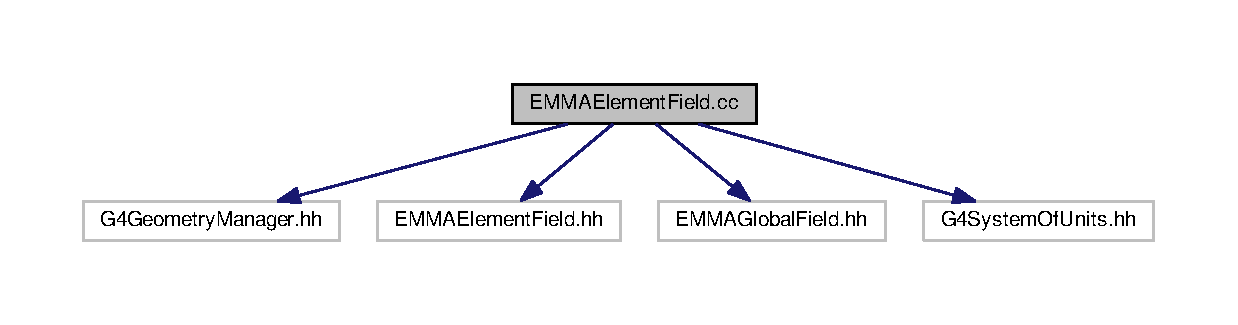
\includegraphics[width=350pt]{EMMAElementField_8cc__incl}
\end{center}
\end{figure}

\hypertarget{EMMAEMPhysics_8cc}{\section{E\-M\-M\-A\-E\-M\-Physics.\-cc File Reference}
\label{EMMAEMPhysics_8cc}\index{E\-M\-M\-A\-E\-M\-Physics.\-cc@{E\-M\-M\-A\-E\-M\-Physics.\-cc}}
}


Defines E\-M physics process functions and particles.  


{\ttfamily \#include \char`\"{}E\-M\-M\-A\-E\-M\-Physics.\-hh\char`\"{}}\\*
{\ttfamily \#include \char`\"{}globals.\-hh\char`\"{}}\\*
{\ttfamily \#include \char`\"{}G4ios.\-hh\char`\"{}}\\*
{\ttfamily \#include $<$iomanip$>$}\\*
{\ttfamily \#include \char`\"{}G4\-Particle\-Definition.\-hh\char`\"{}}\\*
{\ttfamily \#include \char`\"{}G4\-Particle\-Table.\-hh\char`\"{}}\\*
{\ttfamily \#include \char`\"{}G4\-Gamma.\-hh\char`\"{}}\\*
{\ttfamily \#include \char`\"{}G4\-Electron.\-hh\char`\"{}}\\*
{\ttfamily \#include \char`\"{}G4\-Positron.\-hh\char`\"{}}\\*
{\ttfamily \#include \char`\"{}G4\-Neutrino\-E.\-hh\char`\"{}}\\*
{\ttfamily \#include \char`\"{}G4\-Anti\-Neutrino\-E.\-hh\char`\"{}}\\*
{\ttfamily \#include \char`\"{}G4\-Process\-Manager.\-hh\char`\"{}}\\*


\subsection{Detailed Description}
Defines E\-M physics process functions and particles. 
\hypertarget{EMMAEventAction_8cc}{\section{E\-M\-M\-A\-Event\-Action.\-cc File Reference}
\label{EMMAEventAction_8cc}\index{E\-M\-M\-A\-Event\-Action.\-cc@{E\-M\-M\-A\-Event\-Action.\-cc}}
}


Takes care of the interactions (events) of an object that was generated in the Primary Generator. Note\-: If you are getting error messages concerning this file while building E\-M\-M\-A it is likely an error or problem in your (C\-E\-R\-N) R\-O\-O\-T installation, as this file calls upon R\-O\-O\-T functions. Reinstall or remake R\-O\-O\-T, or seek your local computer guru for help.  


{\ttfamily \#include \char`\"{}E\-M\-M\-A\-Event\-Action.\-hh\char`\"{}}\\*
{\ttfamily \#include \char`\"{}E\-M\-M\-A\-Event\-Action\-Messenger.\-hh\char`\"{}}\\*
{\ttfamily \#include \char`\"{}G4\-System\-Of\-Units.\-hh\char`\"{}}\\*
{\ttfamily \#include \char`\"{}G4\-Units\-Table.\-hh\char`\"{}}\\*
{\ttfamily \#include \char`\"{}G4\-Event.\-hh\char`\"{}}\\*
{\ttfamily \#include \char`\"{}G4\-Event\-Manager.\-hh\char`\"{}}\\*
{\ttfamily \#include \char`\"{}G4\-H\-Cof\-This\-Event.\-hh\char`\"{}}\\*
{\ttfamily \#include \char`\"{}G4\-V\-Hits\-Collection.\-hh\char`\"{}}\\*
{\ttfamily \#include \char`\"{}G4\-Trajectory\-Container.\-hh\char`\"{}}\\*
{\ttfamily \#include \char`\"{}G4\-Trajectory.\-hh\char`\"{}}\\*
{\ttfamily \#include \char`\"{}G4\-V\-Vis\-Manager.\-hh\char`\"{}}\\*
{\ttfamily \#include \char`\"{}G4\-S\-D\-Manager.\-hh\char`\"{}}\\*
{\ttfamily \#include \char`\"{}G4\-U\-Imanager.\-hh\char`\"{}}\\*
{\ttfamily \#include \char`\"{}G4ios.\-hh\char`\"{}}\\*
{\ttfamily \#include \char`\"{}E\-M\-M\-A\-Drift\-Chamber\-Hit.\-hh\char`\"{}}\\*
{\ttfamily \#include \char`\"{}E\-M\-M\-A\-Ion\-Chamber.\-hh\char`\"{}}\\*
{\ttfamily \#include \char`\"{}E\-M\-M\-A\-Ion\-Chamber\-Hit.\-hh\char`\"{}}\\*
\subsection*{Variables}
\begin{DoxyCompactItemize}
\item 
\hypertarget{EMMAEventAction_8cc_a8558631b93942e4ae79b3feb21c97c8f}{G4\-String {\bfseries User\-Dir}}\label{EMMAEventAction_8cc_a8558631b93942e4ae79b3feb21c97c8f}

\end{DoxyCompactItemize}


\subsection{Detailed Description}
Takes care of the interactions (events) of an object that was generated in the Primary Generator. Note\-: If you are getting error messages concerning this file while building E\-M\-M\-A it is likely an error or problem in your (C\-E\-R\-N) R\-O\-O\-T installation, as this file calls upon R\-O\-O\-T functions. Reinstall or remake R\-O\-O\-T, or seek your local computer guru for help. 
\hypertarget{EMMAEventActionMessenger_8cc}{}\section{E\+M\+M\+A\+Event\+Action\+Messenger.\+cc File Reference}
\label{EMMAEventActionMessenger_8cc}\index{E\+M\+M\+A\+Event\+Action\+Messenger.\+cc@{E\+M\+M\+A\+Event\+Action\+Messenger.\+cc}}
{\ttfamily \#include \char`\"{}E\+M\+M\+A\+Event\+Action\+Messenger.\+hh\char`\"{}}\\*
{\ttfamily \#include \char`\"{}E\+M\+M\+A\+Event\+Action.\+hh\char`\"{}}\\*
{\ttfamily \#include \char`\"{}G4\+U\+Icmd\+With\+An\+Integer.\+hh\char`\"{}}\\*
{\ttfamily \#include \char`\"{}G4ios.\+hh\char`\"{}}\\*
Include dependency graph for E\+M\+M\+A\+Event\+Action\+Messenger.\+cc\+:
\nopagebreak
\begin{figure}[H]
\begin{center}
\leavevmode
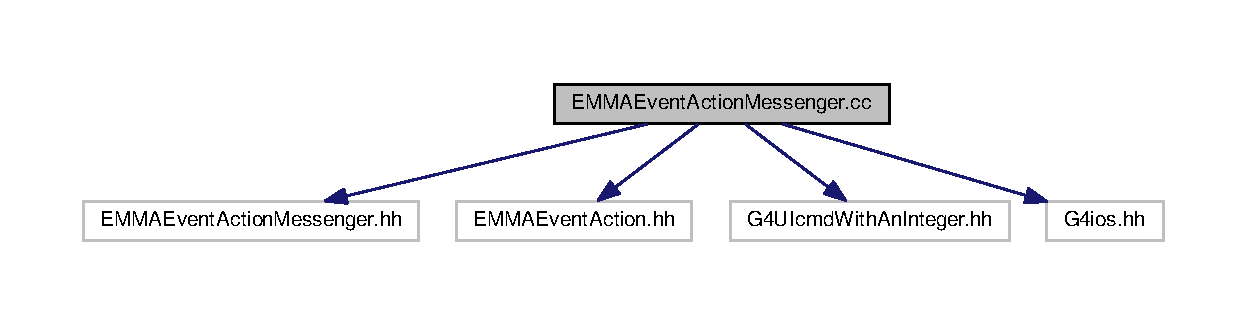
\includegraphics[width=350pt]{EMMAEventActionMessenger_8cc__incl}
\end{center}
\end{figure}

\hypertarget{EMMAGeneralPhysics_8cc}{}\section{E\+M\+M\+A\+General\+Physics.\+cc File Reference}
\label{EMMAGeneralPhysics_8cc}\index{E\+M\+M\+A\+General\+Physics.\+cc@{E\+M\+M\+A\+General\+Physics.\+cc}}
{\ttfamily \#include \char`\"{}E\+M\+M\+A\+General\+Physics.\+hh\char`\"{}}\\*
{\ttfamily \#include \char`\"{}G4\+System\+Of\+Units.\+hh\char`\"{}}\\*
{\ttfamily \#include \char`\"{}globals.\+hh\char`\"{}}\\*
{\ttfamily \#include \char`\"{}G4ios.\+hh\char`\"{}}\\*
{\ttfamily \#include $<$iomanip$>$}\\*
{\ttfamily \#include \char`\"{}F04\+Step\+Max.\+hh\char`\"{}}\\*
{\ttfamily \#include \char`\"{}G4\+Baryon\+Constructor.\+hh\char`\"{}}\\*
{\ttfamily \#include \char`\"{}G4\+Boson\+Constructor.\+hh\char`\"{}}\\*
{\ttfamily \#include \char`\"{}G4\+Ion\+Constructor.\+hh\char`\"{}}\\*
{\ttfamily \#include \char`\"{}G4\+Lepton\+Constructor.\+hh\char`\"{}}\\*
{\ttfamily \#include \char`\"{}G4\+Meson\+Constructor.\+hh\char`\"{}}\\*
{\ttfamily \#include \char`\"{}G4\+Short\+Lived\+Constructor.\+hh\char`\"{}}\\*
{\ttfamily \#include \char`\"{}G4\+Decay.\+hh\char`\"{}}\\*
{\ttfamily \#include \char`\"{}G4\+Particle\+Definition.\+hh\char`\"{}}\\*
{\ttfamily \#include \char`\"{}G4\+Process\+Manager.\+hh\char`\"{}}\\*
{\ttfamily \#include \char`\"{}G4\+Particle\+Table.\+hh\char`\"{}}\\*
{\ttfamily \#include \char`\"{}G4\+V\+User\+Physics\+List.\+hh\char`\"{}}\\*
Include dependency graph for E\+M\+M\+A\+General\+Physics.\+cc\+:
\nopagebreak
\begin{figure}[H]
\begin{center}
\leavevmode
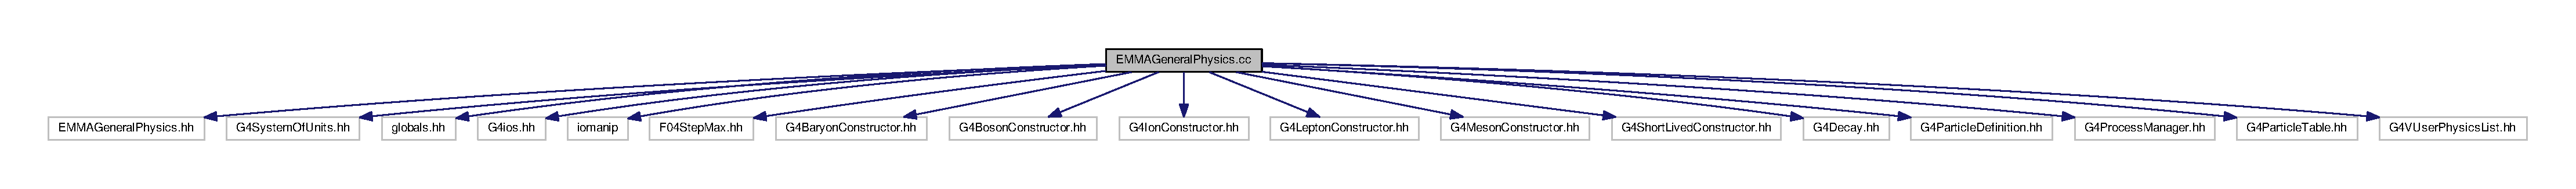
\includegraphics[width=350pt]{EMMAGeneralPhysics_8cc__incl}
\end{center}
\end{figure}

\hypertarget{EMMAGlobalField_8cc}{\section{E\-M\-M\-A\-Global\-Field.\-cc File Reference}
\label{EMMAGlobalField_8cc}\index{E\-M\-M\-A\-Global\-Field.\-cc@{E\-M\-M\-A\-Global\-Field.\-cc}}
}


F04\-Global\-Field -\/ handles the global Electro\-Magnetic field.  


{\ttfamily \#include $<$time.\-h$>$}\\*
{\ttfamily \#include \char`\"{}Randomize.\-hh\char`\"{}}\\*
{\ttfamily \#include \char`\"{}G4\-Transportation\-Manager.\-hh\char`\"{}}\\*
{\ttfamily \#include \char`\"{}G4\-Explicit\-Euler.\-hh\char`\"{}}\\*
{\ttfamily \#include \char`\"{}G4\-Implicit\-Euler.\-hh\char`\"{}}\\*
{\ttfamily \#include \char`\"{}G4\-Simple\-Runge.\-hh\char`\"{}}\\*
{\ttfamily \#include \char`\"{}G4\-Simple\-Heum.\-hh\char`\"{}}\\*
{\ttfamily \#include \char`\"{}G4\-Classical\-R\-K4.\-hh\char`\"{}}\\*
{\ttfamily \#include \char`\"{}G4\-Cash\-Karp\-R\-K\-F45.\-hh\char`\"{}}\\*
{\ttfamily \#include \char`\"{}G4\-System\-Of\-Units.\-hh\char`\"{}}\\*
{\ttfamily \#include \char`\"{}E\-M\-M\-A\-Global\-Field.\-hh\char`\"{}}\\*
{\ttfamily \#include \char`\"{}E\-M\-M\-A\-Element\-Field.\-hh\char`\"{}}\\*
{\ttfamily \#include \char`\"{}E\-M\-Field\-Debugger.\-hh\char`\"{}}\\*


\subsection{Detailed Description}
F04\-Global\-Field -\/ handles the global Electro\-Magnetic field. The field from each individual beamline element (quad, E\-D, etc.) is given by a Element\-Field object. Any number of overlapping Element\-Field objects can be added to the global field. Any element with an E\-M field must add the appropriate Element\-Field to the global Global\-Field object. There is a single G04\-Global\-Field object. 
\hypertarget{EMMAHadronPhysics_8cc}{}\section{E\+M\+M\+A\+Hadron\+Physics.\+cc File Reference}
\label{EMMAHadronPhysics_8cc}\index{E\+M\+M\+A\+Hadron\+Physics.\+cc@{E\+M\+M\+A\+Hadron\+Physics.\+cc}}
{\ttfamily \#include \char`\"{}E\+M\+M\+A\+Hadron\+Physics.\+hh\char`\"{}}\\*
{\ttfamily \#include \char`\"{}globals.\+hh\char`\"{}}\\*
{\ttfamily \#include \char`\"{}G4ios.\+hh\char`\"{}}\\*
{\ttfamily \#include $<$iomanip$>$}\\*
{\ttfamily \#include \char`\"{}G4\+Particle\+Definition.\+hh\char`\"{}}\\*
{\ttfamily \#include \char`\"{}G4\+Particle\+Table.\+hh\char`\"{}}\\*
{\ttfamily \#include \char`\"{}G4\+Process\+Manager.\+hh\char`\"{}}\\*
Include dependency graph for E\+M\+M\+A\+Hadron\+Physics.\+cc\+:
\nopagebreak
\begin{figure}[H]
\begin{center}
\leavevmode
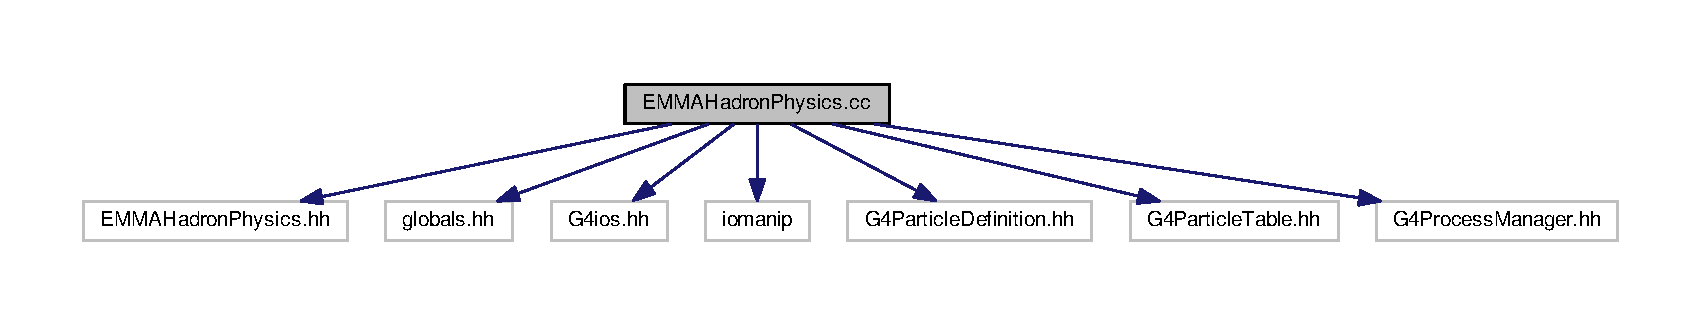
\includegraphics[width=350pt]{EMMAHadronPhysics_8cc__incl}
\end{center}
\end{figure}

\hypertarget{EMMAIonChamber_8cc}{\section{E\-M\-M\-A\-Ion\-Chamber.\-cc File Reference}
\label{EMMAIonChamber_8cc}\index{E\-M\-M\-A\-Ion\-Chamber.\-cc@{E\-M\-M\-A\-Ion\-Chamber.\-cc}}
}


Implementation of the B4c\-Calorimeter\-S\-D class Builds the ion chamber and defines the types of data it outputs. Look here to modify the specific workings of the I\-C. (Look also in Detector\-Construction)  


{\ttfamily \#include \char`\"{}E\-M\-M\-A\-Ion\-Chamber.\-hh\char`\"{}}\\*
{\ttfamily \#include \char`\"{}G4\-H\-Cof\-This\-Event.\-hh\char`\"{}}\\*
{\ttfamily \#include \char`\"{}G4\-Step.\-hh\char`\"{}}\\*
{\ttfamily \#include \char`\"{}G4\-Three\-Vector.\-hh\char`\"{}}\\*
{\ttfamily \#include \char`\"{}G4\-S\-D\-Manager.\-hh\char`\"{}}\\*
{\ttfamily \#include \char`\"{}G4ios.\-hh\char`\"{}}\\*


\subsection{Detailed Description}
Implementation of the B4c\-Calorimeter\-S\-D class Builds the ion chamber and defines the types of data it outputs. Look here to modify the specific workings of the I\-C. (Look also in Detector\-Construction) 
\hypertarget{EMMAIonChamberHit_8cc}{}\section{E\+M\+M\+A\+Ion\+Chamber\+Hit.\+cc File Reference}
\label{EMMAIonChamberHit_8cc}\index{E\+M\+M\+A\+Ion\+Chamber\+Hit.\+cc@{E\+M\+M\+A\+Ion\+Chamber\+Hit.\+cc}}
{\ttfamily \#include \char`\"{}E\+M\+M\+A\+Ion\+Chamber\+Hit.\+hh\char`\"{}}\\*
{\ttfamily \#include \char`\"{}G4\+Units\+Table.\+hh\char`\"{}}\\*
{\ttfamily \#include \char`\"{}G4\+V\+Vis\+Manager.\+hh\char`\"{}}\\*
{\ttfamily \#include \char`\"{}G4\+Circle.\+hh\char`\"{}}\\*
{\ttfamily \#include \char`\"{}G4\+Colour.\+hh\char`\"{}}\\*
{\ttfamily \#include \char`\"{}G4\+Vis\+Attributes.\+hh\char`\"{}}\\*
{\ttfamily \#include $<$iomanip$>$}\\*
Include dependency graph for E\+M\+M\+A\+Ion\+Chamber\+Hit.\+cc\+:
\nopagebreak
\begin{figure}[H]
\begin{center}
\leavevmode
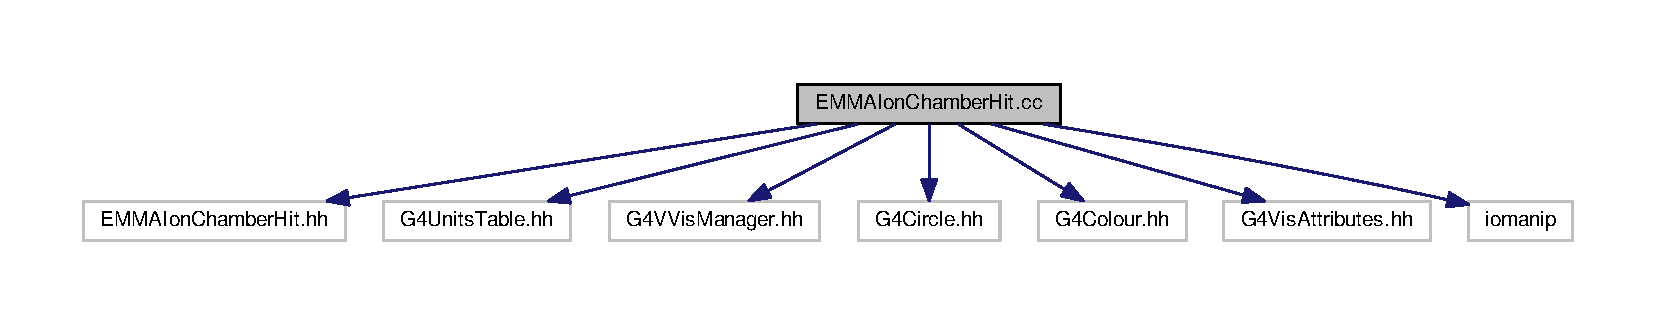
\includegraphics[width=350pt]{EMMAIonChamberHit_8cc__incl}
\end{center}
\end{figure}
\subsection*{Variables}
\begin{DoxyCompactItemize}
\item 
G4\+Allocator$<$ E\+M\+M\+A\+Ion\+Chamber\+Hit $>$ \hyperlink{EMMAIonChamberHit_8cc_adb78e92d0fb21fc2a8a5f8f8d03805ea}{E\+M\+M\+A\+Ion\+Chamber\+Hit\+Allocator}
\end{DoxyCompactItemize}


\subsection{Variable Documentation}
\index{E\+M\+M\+A\+Ion\+Chamber\+Hit.\+cc@{E\+M\+M\+A\+Ion\+Chamber\+Hit.\+cc}!E\+M\+M\+A\+Ion\+Chamber\+Hit\+Allocator@{E\+M\+M\+A\+Ion\+Chamber\+Hit\+Allocator}}
\index{E\+M\+M\+A\+Ion\+Chamber\+Hit\+Allocator@{E\+M\+M\+A\+Ion\+Chamber\+Hit\+Allocator}!E\+M\+M\+A\+Ion\+Chamber\+Hit.\+cc@{E\+M\+M\+A\+Ion\+Chamber\+Hit.\+cc}}
\subsubsection[{\texorpdfstring{E\+M\+M\+A\+Ion\+Chamber\+Hit\+Allocator}{EMMAIonChamberHitAllocator}}]{\setlength{\rightskip}{0pt plus 5cm}G4\+Allocator$<$E\+M\+M\+A\+Ion\+Chamber\+Hit$>$ E\+M\+M\+A\+Ion\+Chamber\+Hit\+Allocator}\hypertarget{EMMAIonChamberHit_8cc_adb78e92d0fb21fc2a8a5f8f8d03805ea}{}\label{EMMAIonChamberHit_8cc_adb78e92d0fb21fc2a8a5f8f8d03805ea}

\hypertarget{EMMAIonPhysics_8cc}{}\section{E\+M\+M\+A\+Ion\+Physics.\+cc File Reference}
\label{EMMAIonPhysics_8cc}\index{E\+M\+M\+A\+Ion\+Physics.\+cc@{E\+M\+M\+A\+Ion\+Physics.\+cc}}
{\ttfamily \#include \char`\"{}E\+M\+M\+A\+Ion\+Physics.\+hh\char`\"{}}\\*
{\ttfamily \#include \char`\"{}globals.\+hh\char`\"{}}\\*
{\ttfamily \#include \char`\"{}G4ios.\+hh\char`\"{}}\\*
{\ttfamily \#include $<$iomanip$>$}\\*
{\ttfamily \#include \char`\"{}G4\+Region.\+hh\char`\"{}}\\*
{\ttfamily \#include \char`\"{}G4\+Region\+Store.\+hh\char`\"{}}\\*
{\ttfamily \#include \char`\"{}G4\+Production\+Cuts.\+hh\char`\"{}}\\*
{\ttfamily \#include \char`\"{}G4\+Em\+Configurator.\+hh\char`\"{}}\\*
{\ttfamily \#include \char`\"{}G4\+Loss\+Table\+Manager.\+hh\char`\"{}}\\*
{\ttfamily \#include \char`\"{}G4\+Bragg\+Ion\+Gas\+Model.\+hh\char`\"{}}\\*
{\ttfamily \#include \char`\"{}G4\+Bethe\+Bloch\+Ion\+Gas\+Model.\+hh\char`\"{}}\\*
{\ttfamily \#include \char`\"{}G4\+Ion\+Fluctuations.\+hh\char`\"{}}\\*
{\ttfamily \#include \char`\"{}G4\+Universal\+Fluctuation.\+hh\char`\"{}}\\*
{\ttfamily \#include \char`\"{}G4\+Particle\+Definition.\+hh\char`\"{}}\\*
{\ttfamily \#include \char`\"{}G4\+Particle\+Table.\+hh\char`\"{}}\\*
{\ttfamily \#include \char`\"{}G4\+Process\+Manager.\+hh\char`\"{}}\\*
{\ttfamily \#include \char`\"{}G4\+Em\+Process\+Options.\+hh\char`\"{}}\\*
{\ttfamily \#include \char`\"{}G4\+Ion\+Parametrised\+Loss\+Model.\+hh\char`\"{}}\\*
{\ttfamily \#include \char`\"{}G4\+Nuclear\+Stopping.\+hh\char`\"{}}\\*
{\ttfamily \#include \char`\"{}G4\+Urban\+Msc\+Model90.\+hh\char`\"{}}\\*
{\ttfamily \#include \char`\"{}G4\+Urban\+Msc\+Model95.\+hh\char`\"{}}\\*
{\ttfamily \#include \char`\"{}G4\+Wentzel\+V\+I\+Model.\+hh\char`\"{}}\\*
{\ttfamily \#include \char`\"{}G4\+Coulomb\+Scattering.\+hh\char`\"{}}\\*
{\ttfamily \#include \char`\"{}G4\+Ion\+Coulomb\+Scattering\+Model.\+hh\char`\"{}}\\*
{\ttfamily \#include \char`\"{}G4\+Screened\+Nuclear\+Recoil.\+hh\char`\"{}}\\*
{\ttfamily \#include \char`\"{}E\+M\+M\+A\+Ion\+Physics\+Messenger.\+hh\char`\"{}}\\*
Include dependency graph for E\+M\+M\+A\+Ion\+Physics.\+cc\+:
\nopagebreak
\begin{figure}[H]
\begin{center}
\leavevmode
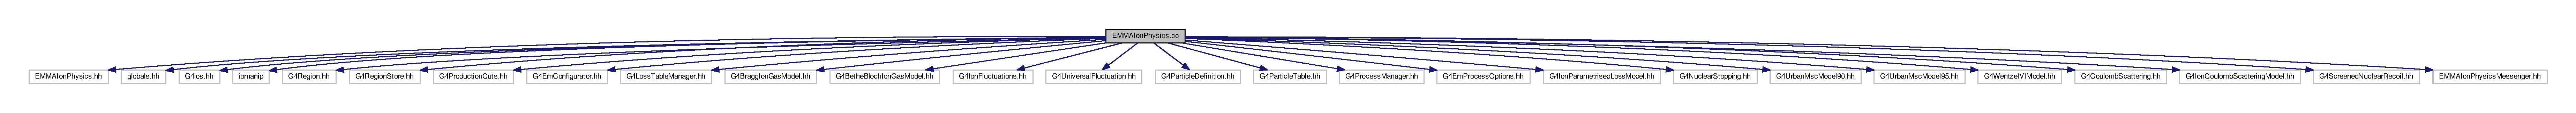
\includegraphics[width=350pt]{EMMAIonPhysics_8cc__incl}
\end{center}
\end{figure}

\hypertarget{EMMAIonPhysicsMessenger_8cc}{\section{E\-M\-M\-A\-Ion\-Physics\-Messenger.\-cc File Reference}
\label{EMMAIonPhysicsMessenger_8cc}\index{E\-M\-M\-A\-Ion\-Physics\-Messenger.\-cc@{E\-M\-M\-A\-Ion\-Physics\-Messenger.\-cc}}
}


Connects and delivers user commands regarding ion physics particles and processes to respective classes, and relays their responses to the user.  


{\ttfamily \#include \char`\"{}E\-M\-M\-A\-Ion\-Physics\-Messenger.\-hh\char`\"{}}\\*
{\ttfamily \#include \char`\"{}E\-M\-M\-A\-Ion\-Physics.\-hh\char`\"{}}\\*
{\ttfamily \#include \char`\"{}G4\-U\-Icmd\-With\-A\-Double\-And\-Unit.\-hh\char`\"{}}\\*
{\ttfamily \#include \char`\"{}G4\-U\-Icmd\-With\-A\-Double.\-hh\char`\"{}}\\*
{\ttfamily \#include \char`\"{}G4\-U\-Icmd\-With\-A\-Bool.\-hh\char`\"{}}\\*
{\ttfamily \#include \char`\"{}G4ios.\-hh\char`\"{}}\\*


\subsection{Detailed Description}
Connects and delivers user commands regarding ion physics particles and processes to respective classes, and relays their responses to the user. 
\hypertarget{EMMAMuonPhysics_8cc}{}\section{E\+M\+M\+A\+Muon\+Physics.\+cc File Reference}
\label{EMMAMuonPhysics_8cc}\index{E\+M\+M\+A\+Muon\+Physics.\+cc@{E\+M\+M\+A\+Muon\+Physics.\+cc}}
{\ttfamily \#include \char`\"{}E\+M\+M\+A\+Muon\+Physics.\+hh\char`\"{}}\\*
{\ttfamily \#include \char`\"{}globals.\+hh\char`\"{}}\\*
{\ttfamily \#include \char`\"{}G4ios.\+hh\char`\"{}}\\*
{\ttfamily \#include $<$iomanip$>$}\\*
{\ttfamily \#include \char`\"{}G4\+Particle\+Definition.\+hh\char`\"{}}\\*
{\ttfamily \#include \char`\"{}G4\+Particle\+Table.\+hh\char`\"{}}\\*
{\ttfamily \#include \char`\"{}G4\+Muon\+Plus.\+hh\char`\"{}}\\*
{\ttfamily \#include \char`\"{}G4\+Muon\+Minus.\+hh\char`\"{}}\\*
{\ttfamily \#include \char`\"{}G4\+Tau\+Minus.\+hh\char`\"{}}\\*
{\ttfamily \#include \char`\"{}G4\+Tau\+Plus.\+hh\char`\"{}}\\*
{\ttfamily \#include \char`\"{}G4\+Process\+Manager.\+hh\char`\"{}}\\*
Include dependency graph for E\+M\+M\+A\+Muon\+Physics.\+cc\+:
\nopagebreak
\begin{figure}[H]
\begin{center}
\leavevmode
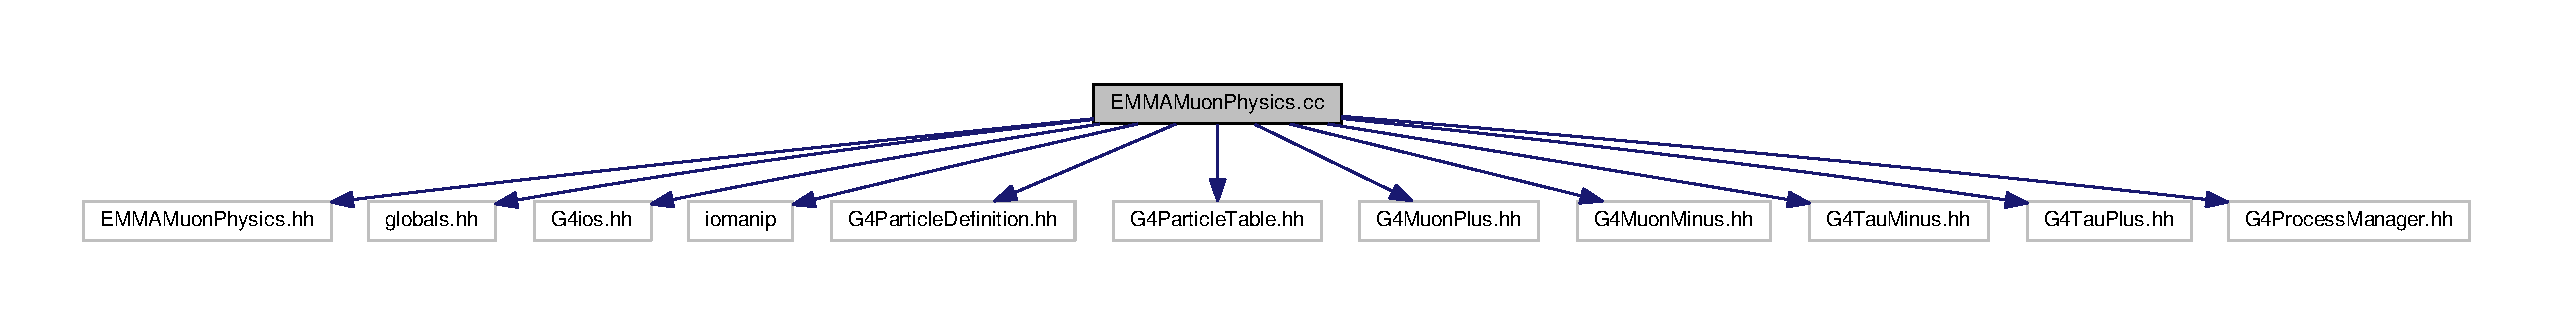
\includegraphics[width=350pt]{EMMAMuonPhysics_8cc__incl}
\end{center}
\end{figure}

\hypertarget{EMMANuclearReactionDataSet_8cc}{}\section{E\+M\+M\+A\+Nuclear\+Reaction\+Data\+Set.\+cc File Reference}
\label{EMMANuclearReactionDataSet_8cc}\index{E\+M\+M\+A\+Nuclear\+Reaction\+Data\+Set.\+cc@{E\+M\+M\+A\+Nuclear\+Reaction\+Data\+Set.\+cc}}
{\ttfamily \#include \char`\"{}G4\+Nist\+Manager.\+hh\char`\"{}}\\*
{\ttfamily \#include \char`\"{}G4\+Had\+Tmp\+Util.\+hh\char`\"{}}\\*
{\ttfamily \#include $<$iostream$>$}\\*
{\ttfamily \#include \char`\"{}E\+M\+M\+A\+Nuclear\+Reaction\+Data\+Set.\+hh\char`\"{}}\\*
Include dependency graph for E\+M\+M\+A\+Nuclear\+Reaction\+Data\+Set.\+cc\+:
\nopagebreak
\begin{figure}[H]
\begin{center}
\leavevmode
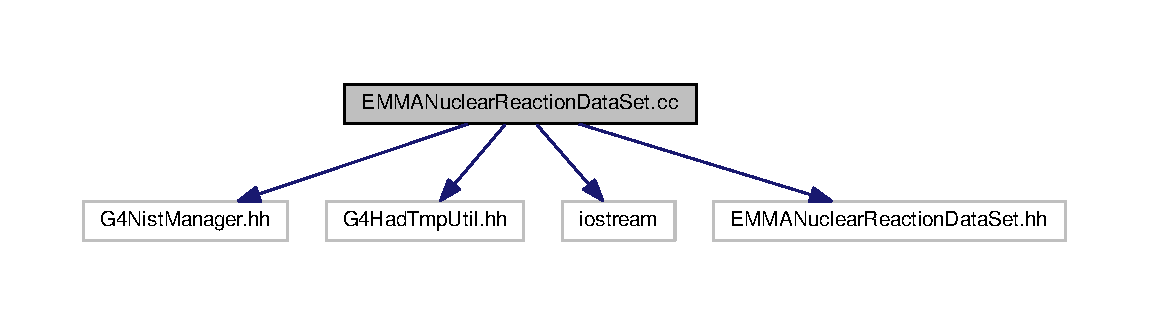
\includegraphics[width=350pt]{EMMANuclearReactionDataSet_8cc__incl}
\end{center}
\end{figure}

\hypertarget{EMMANuclearReactionProcess_8cc}{}\section{E\+M\+M\+A\+Nuclear\+Reaction\+Process.\+cc File Reference}
\label{EMMANuclearReactionProcess_8cc}\index{E\+M\+M\+A\+Nuclear\+Reaction\+Process.\+cc@{E\+M\+M\+A\+Nuclear\+Reaction\+Process.\+cc}}
{\ttfamily \#include $<$iostream$>$}\\*
{\ttfamily \#include $<$typeinfo$>$}\\*
{\ttfamily \#include \char`\"{}G4\+System\+Of\+Units.\+hh\char`\"{}}\\*
{\ttfamily \#include \char`\"{}G4\+Nucleus.\+hh\char`\"{}}\\*
{\ttfamily \#include \char`\"{}G4\+Process\+Manager.\+hh\char`\"{}}\\*
{\ttfamily \#include \char`\"{}G4\+Cross\+Section\+Data\+Store.\+hh\char`\"{}}\\*
{\ttfamily \#include \char`\"{}E\+M\+M\+A\+Nuclear\+Reaction\+Data\+Set.\+hh\char`\"{}}\\*
{\ttfamily \#include \char`\"{}G4\+Production\+Cuts\+Table.\+hh\char`\"{}}\\*
{\ttfamily \#include \char`\"{}G4\+Hadronic\+Exception.\+hh\char`\"{}}\\*
{\ttfamily \#include \char`\"{}G4\+Hadronic\+Deprecate.\+hh\char`\"{}}\\*
{\ttfamily \#include \char`\"{}E\+M\+M\+A\+Nuclear\+Reaction\+Process.\+hh\char`\"{}}\\*
{\ttfamily \#include \char`\"{}E\+M\+M\+A\+Nuclear\+Reaction\+Two\+Body.\+hh\char`\"{}}\\*
Include dependency graph for E\+M\+M\+A\+Nuclear\+Reaction\+Process.\+cc\+:
\nopagebreak
\begin{figure}[H]
\begin{center}
\leavevmode
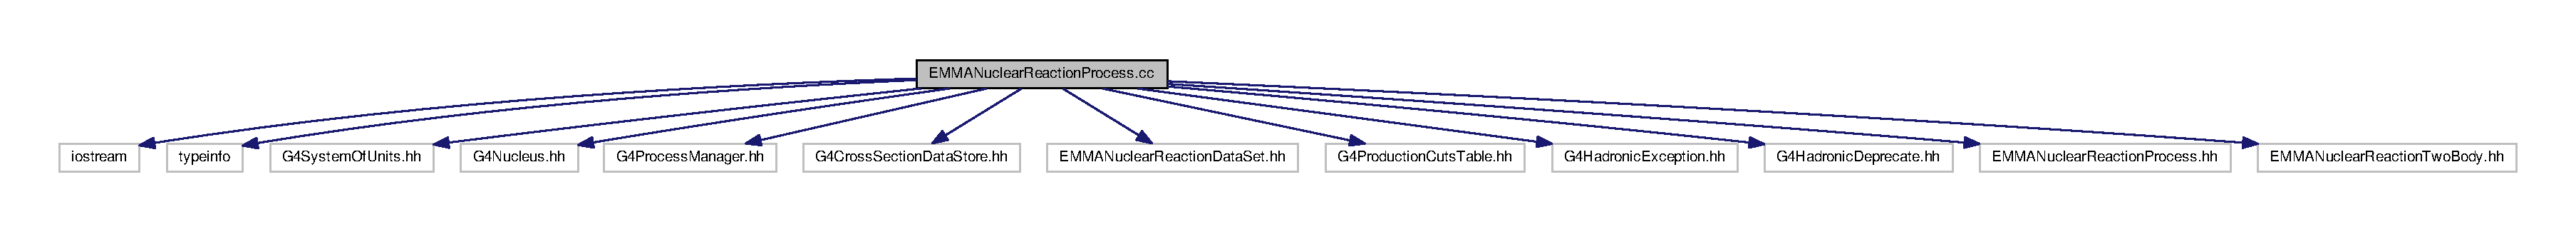
\includegraphics[width=350pt]{EMMANuclearReactionProcess_8cc__incl}
\end{center}
\end{figure}

\hypertarget{EMMANuclearReactionTwoBody_8cc}{}\section{E\+M\+M\+A\+Nuclear\+Reaction\+Two\+Body.\+cc File Reference}
\label{EMMANuclearReactionTwoBody_8cc}\index{E\+M\+M\+A\+Nuclear\+Reaction\+Two\+Body.\+cc@{E\+M\+M\+A\+Nuclear\+Reaction\+Two\+Body.\+cc}}
{\ttfamily \#include $<$iostream$>$}\\*
{\ttfamily \#include \char`\"{}E\+M\+M\+A\+Nuclear\+Reaction\+Two\+Body.\+hh\char`\"{}}\\*
{\ttfamily \#include \char`\"{}globals.\+hh\char`\"{}}\\*
{\ttfamily \#include \char`\"{}G4\+Physical\+Constants.\+hh\char`\"{}}\\*
{\ttfamily \#include \char`\"{}G4\+System\+Of\+Units.\+hh\char`\"{}}\\*
{\ttfamily \#include \char`\"{}Randomize.\+hh\char`\"{}}\\*
{\ttfamily \#include \char`\"{}G4\+Particle\+Table.\+hh\char`\"{}}\\*
{\ttfamily \#include \char`\"{}G4\+Ion\+Table.\+hh\char`\"{}}\\*
{\ttfamily \#include \char`\"{}G4\+Proton.\+hh\char`\"{}}\\*
{\ttfamily \#include \char`\"{}G4\+Neutron.\+hh\char`\"{}}\\*
{\ttfamily \#include \char`\"{}G4\+Deuteron.\+hh\char`\"{}}\\*
{\ttfamily \#include \char`\"{}G4\+Triton.\+hh\char`\"{}}\\*
{\ttfamily \#include \char`\"{}G4\+Alpha.\+hh\char`\"{}}\\*
{\ttfamily \#include \char`\"{}G4\+He3.\+hh\char`\"{}}\\*
{\ttfamily \#include \char`\"{}G4\+Gamma.\+hh\char`\"{}}\\*
{\ttfamily \#include \char`\"{}G4\+Nuclei\+Properties.\+hh\char`\"{}}\\*
Include dependency graph for E\+M\+M\+A\+Nuclear\+Reaction\+Two\+Body.\+cc\+:
\nopagebreak
\begin{figure}[H]
\begin{center}
\leavevmode
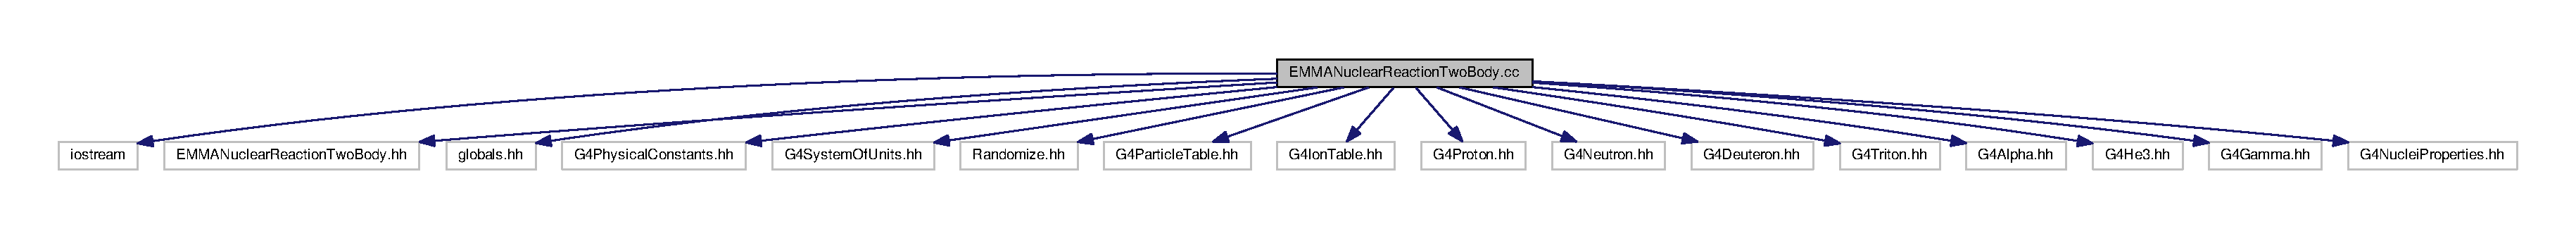
\includegraphics[width=350pt]{EMMANuclearReactionTwoBody_8cc__incl}
\end{center}
\end{figure}

\hypertarget{EMMAPhysicsList_8cc}{}\section{E\+M\+M\+A\+Physics\+List.\+cc File Reference}
\label{EMMAPhysicsList_8cc}\index{E\+M\+M\+A\+Physics\+List.\+cc@{E\+M\+M\+A\+Physics\+List.\+cc}}
{\ttfamily \#include \char`\"{}E\+M\+M\+A\+Physics\+List.\+hh\char`\"{}}\\*
{\ttfamily \#include \char`\"{}globals.\+hh\char`\"{}}\\*
{\ttfamily \#include \char`\"{}G4\+Particle\+Definition.\+hh\char`\"{}}\\*
{\ttfamily \#include \char`\"{}G4\+Particle\+With\+Cuts.\+hh\char`\"{}}\\*
{\ttfamily \#include \char`\"{}G4\+Process\+Manager.\+hh\char`\"{}}\\*
{\ttfamily \#include \char`\"{}G4\+Process\+Vector.\+hh\char`\"{}}\\*
{\ttfamily \#include \char`\"{}G4\+Particle\+Types.\+hh\char`\"{}}\\*
{\ttfamily \#include \char`\"{}G4\+Particle\+Table.\+hh\char`\"{}}\\*
{\ttfamily \#include \char`\"{}G4\+Material.\+hh\char`\"{}}\\*
{\ttfamily \#include \char`\"{}G4\+Material\+Table.\+hh\char`\"{}}\\*
{\ttfamily \#include \char`\"{}G4ios.\+hh\char`\"{}}\\*
{\ttfamily \#include $<$iomanip$>$}\\*
{\ttfamily \#include \char`\"{}E\+M\+M\+A\+General\+Physics.\+hh\char`\"{}}\\*
{\ttfamily \#include \char`\"{}E\+M\+M\+A\+E\+M\+Physics.\+hh\char`\"{}}\\*
{\ttfamily \#include \char`\"{}E\+M\+M\+A\+Muon\+Physics.\+hh\char`\"{}}\\*
{\ttfamily \#include \char`\"{}E\+M\+M\+A\+Hadron\+Physics.\+hh\char`\"{}}\\*
{\ttfamily \#include \char`\"{}E\+M\+M\+A\+Ion\+Physics.\+hh\char`\"{}}\\*
Include dependency graph for E\+M\+M\+A\+Physics\+List.\+cc\+:
\nopagebreak
\begin{figure}[H]
\begin{center}
\leavevmode
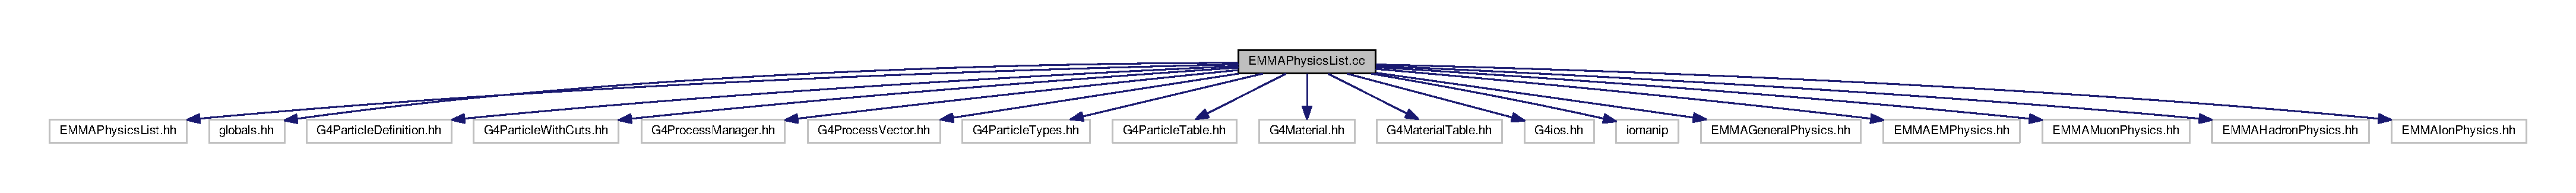
\includegraphics[width=350pt]{EMMAPhysicsList_8cc__incl}
\end{center}
\end{figure}

\hypertarget{EMMAPrimaryGeneratorAction_8cc}{}\section{E\+M\+M\+A\+Primary\+Generator\+Action.\+cc File Reference}
\label{EMMAPrimaryGeneratorAction_8cc}\index{E\+M\+M\+A\+Primary\+Generator\+Action.\+cc@{E\+M\+M\+A\+Primary\+Generator\+Action.\+cc}}
{\ttfamily \#include \char`\"{}E\+M\+M\+A\+Primary\+Generator\+Action.\+hh\char`\"{}}\\*
{\ttfamily \#include \char`\"{}E\+M\+M\+A\+Primary\+Generator\+Messenger.\+hh\char`\"{}}\\*
{\ttfamily \#include \char`\"{}G4\+Event.\+hh\char`\"{}}\\*
{\ttfamily \#include \char`\"{}G4\+Particle\+Gun.\+hh\char`\"{}}\\*
{\ttfamily \#include \char`\"{}G4\+Particle\+Table.\+hh\char`\"{}}\\*
{\ttfamily \#include \char`\"{}G4\+Particle\+Definition.\+hh\char`\"{}}\\*
{\ttfamily \#include \char`\"{}Randomize.\+hh\char`\"{}}\\*
{\ttfamily \#include \char`\"{}G4ios.\+hh\char`\"{}}\\*
{\ttfamily \#include \char`\"{}G4\+Units\+Table.\+hh\char`\"{}}\\*
{\ttfamily \#include \char`\"{}G4\+Track.\+hh\char`\"{}}\\*
{\ttfamily \#include \char`\"{}G4\+Step.\+hh\char`\"{}}\\*
{\ttfamily \#include \char`\"{}G4\+Particle\+Types.\+hh\char`\"{}}\\*
{\ttfamily \#include \char`\"{}G4\+Physical\+Constants.\+hh\char`\"{}}\\*
{\ttfamily \#include \char`\"{}G4\+System\+Of\+Units.\+hh\char`\"{}}\\*
{\ttfamily \#include \char`\"{}G4\+Ion\+Table.\+hh\char`\"{}}\\*
{\ttfamily \#include \char`\"{}G4\+Nuclei\+Properties.\+hh\char`\"{}}\\*
{\ttfamily \#include \char`\"{}G4\+Gamma.\+hh\char`\"{}}\\*
{\ttfamily \#include \char`\"{}G4\+Run\+Manager.\+hh\char`\"{}}\\*
{\ttfamily \#include \char`\"{}G4\+Logical\+Volume\+Store.\+hh\char`\"{}}\\*
{\ttfamily \#include \char`\"{}G4\+Logical\+Volume.\+hh\char`\"{}}\\*
{\ttfamily \#include \char`\"{}G4\+V\+Solid.\+hh\char`\"{}}\\*
{\ttfamily \#include \char`\"{}G4\+Box.\+hh\char`\"{}}\\*
{\ttfamily \#include $<$string$>$}\\*
{\ttfamily \#include $<$fstream$>$}\\*
{\ttfamily \#include $<$sstream$>$}\\*
Include dependency graph for E\+M\+M\+A\+Primary\+Generator\+Action.\+cc\+:
\nopagebreak
\begin{figure}[H]
\begin{center}
\leavevmode
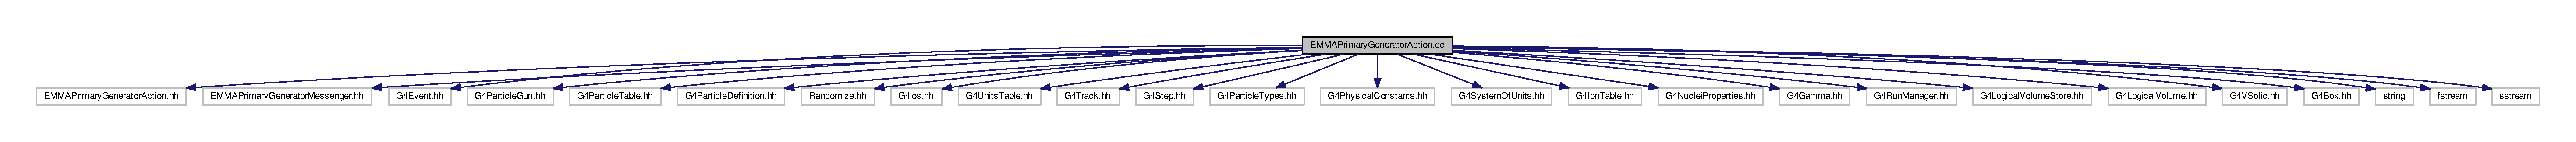
\includegraphics[width=350pt]{EMMAPrimaryGeneratorAction_8cc__incl}
\end{center}
\end{figure}
\subsection*{Variables}
\begin{DoxyCompactItemize}
\item 
G4bool \hyperlink{EMMAPrimaryGeneratorAction_8cc_accd97970a0ee52817a02f8bdf0969668}{prepare\+Beam} = true
\item 
G4\+String \hyperlink{EMMAPrimaryGeneratorAction_8cc_ab5043f10e6a2b6521cf9bdc5f9b50a14}{in\+Target\+File\+Name}
\item 
G4\+String \hyperlink{EMMAPrimaryGeneratorAction_8cc_a44c8e472e5202caa69e70c5e8d18adf7}{post\+Target\+File\+Name}
\item 
G4\+String \hyperlink{EMMAPrimaryGeneratorAction_8cc_a3dbaf7156a8d958508b9806a0ef50aa6}{focal\+Plane\+File\+Name}
\item 
G4double \hyperlink{EMMAPrimaryGeneratorAction_8cc_a2d61cdd1b1b5ed409f7c91b54737c1b9}{user\+Charge} = 54.
\item 
G4\+String \hyperlink{EMMAPrimaryGeneratorAction_8cc_ae92d83921bde0242f8c619b79b457b23}{post\+Degrader1\+File\+Name}
\item 
G4double \hyperlink{EMMAPrimaryGeneratorAction_8cc_a08a40c9f48981a0140f43cbf773f3eea}{depth}
\end{DoxyCompactItemize}


\subsection{Variable Documentation}
\index{E\+M\+M\+A\+Primary\+Generator\+Action.\+cc@{E\+M\+M\+A\+Primary\+Generator\+Action.\+cc}!depth@{depth}}
\index{depth@{depth}!E\+M\+M\+A\+Primary\+Generator\+Action.\+cc@{E\+M\+M\+A\+Primary\+Generator\+Action.\+cc}}
\subsubsection[{\texorpdfstring{depth}{depth}}]{\setlength{\rightskip}{0pt plus 5cm}G4double depth}\hypertarget{EMMAPrimaryGeneratorAction_8cc_a08a40c9f48981a0140f43cbf773f3eea}{}\label{EMMAPrimaryGeneratorAction_8cc_a08a40c9f48981a0140f43cbf773f3eea}
\index{E\+M\+M\+A\+Primary\+Generator\+Action.\+cc@{E\+M\+M\+A\+Primary\+Generator\+Action.\+cc}!focal\+Plane\+File\+Name@{focal\+Plane\+File\+Name}}
\index{focal\+Plane\+File\+Name@{focal\+Plane\+File\+Name}!E\+M\+M\+A\+Primary\+Generator\+Action.\+cc@{E\+M\+M\+A\+Primary\+Generator\+Action.\+cc}}
\subsubsection[{\texorpdfstring{focal\+Plane\+File\+Name}{focalPlaneFileName}}]{\setlength{\rightskip}{0pt plus 5cm}G4\+String focal\+Plane\+File\+Name}\hypertarget{EMMAPrimaryGeneratorAction_8cc_a3dbaf7156a8d958508b9806a0ef50aa6}{}\label{EMMAPrimaryGeneratorAction_8cc_a3dbaf7156a8d958508b9806a0ef50aa6}
\index{E\+M\+M\+A\+Primary\+Generator\+Action.\+cc@{E\+M\+M\+A\+Primary\+Generator\+Action.\+cc}!in\+Target\+File\+Name@{in\+Target\+File\+Name}}
\index{in\+Target\+File\+Name@{in\+Target\+File\+Name}!E\+M\+M\+A\+Primary\+Generator\+Action.\+cc@{E\+M\+M\+A\+Primary\+Generator\+Action.\+cc}}
\subsubsection[{\texorpdfstring{in\+Target\+File\+Name}{inTargetFileName}}]{\setlength{\rightskip}{0pt plus 5cm}G4\+String in\+Target\+File\+Name}\hypertarget{EMMAPrimaryGeneratorAction_8cc_ab5043f10e6a2b6521cf9bdc5f9b50a14}{}\label{EMMAPrimaryGeneratorAction_8cc_ab5043f10e6a2b6521cf9bdc5f9b50a14}
\index{E\+M\+M\+A\+Primary\+Generator\+Action.\+cc@{E\+M\+M\+A\+Primary\+Generator\+Action.\+cc}!post\+Degrader1\+File\+Name@{post\+Degrader1\+File\+Name}}
\index{post\+Degrader1\+File\+Name@{post\+Degrader1\+File\+Name}!E\+M\+M\+A\+Primary\+Generator\+Action.\+cc@{E\+M\+M\+A\+Primary\+Generator\+Action.\+cc}}
\subsubsection[{\texorpdfstring{post\+Degrader1\+File\+Name}{postDegrader1FileName}}]{\setlength{\rightskip}{0pt plus 5cm}G4\+String post\+Degrader1\+File\+Name}\hypertarget{EMMAPrimaryGeneratorAction_8cc_ae92d83921bde0242f8c619b79b457b23}{}\label{EMMAPrimaryGeneratorAction_8cc_ae92d83921bde0242f8c619b79b457b23}
\index{E\+M\+M\+A\+Primary\+Generator\+Action.\+cc@{E\+M\+M\+A\+Primary\+Generator\+Action.\+cc}!post\+Target\+File\+Name@{post\+Target\+File\+Name}}
\index{post\+Target\+File\+Name@{post\+Target\+File\+Name}!E\+M\+M\+A\+Primary\+Generator\+Action.\+cc@{E\+M\+M\+A\+Primary\+Generator\+Action.\+cc}}
\subsubsection[{\texorpdfstring{post\+Target\+File\+Name}{postTargetFileName}}]{\setlength{\rightskip}{0pt plus 5cm}G4\+String post\+Target\+File\+Name}\hypertarget{EMMAPrimaryGeneratorAction_8cc_a44c8e472e5202caa69e70c5e8d18adf7}{}\label{EMMAPrimaryGeneratorAction_8cc_a44c8e472e5202caa69e70c5e8d18adf7}
\index{E\+M\+M\+A\+Primary\+Generator\+Action.\+cc@{E\+M\+M\+A\+Primary\+Generator\+Action.\+cc}!prepare\+Beam@{prepare\+Beam}}
\index{prepare\+Beam@{prepare\+Beam}!E\+M\+M\+A\+Primary\+Generator\+Action.\+cc@{E\+M\+M\+A\+Primary\+Generator\+Action.\+cc}}
\subsubsection[{\texorpdfstring{prepare\+Beam}{prepareBeam}}]{\setlength{\rightskip}{0pt plus 5cm}G4bool prepare\+Beam = true}\hypertarget{EMMAPrimaryGeneratorAction_8cc_accd97970a0ee52817a02f8bdf0969668}{}\label{EMMAPrimaryGeneratorAction_8cc_accd97970a0ee52817a02f8bdf0969668}
\index{E\+M\+M\+A\+Primary\+Generator\+Action.\+cc@{E\+M\+M\+A\+Primary\+Generator\+Action.\+cc}!user\+Charge@{user\+Charge}}
\index{user\+Charge@{user\+Charge}!E\+M\+M\+A\+Primary\+Generator\+Action.\+cc@{E\+M\+M\+A\+Primary\+Generator\+Action.\+cc}}
\subsubsection[{\texorpdfstring{user\+Charge}{userCharge}}]{\setlength{\rightskip}{0pt plus 5cm}G4double user\+Charge = 54.}\hypertarget{EMMAPrimaryGeneratorAction_8cc_a2d61cdd1b1b5ed409f7c91b54737c1b9}{}\label{EMMAPrimaryGeneratorAction_8cc_a2d61cdd1b1b5ed409f7c91b54737c1b9}

\hypertarget{EMMAPrimaryGeneratorMessenger_8cc}{\section{E\-M\-M\-A\-Primary\-Generator\-Messenger.\-cc File Reference}
\label{EMMAPrimaryGeneratorMessenger_8cc}\index{E\-M\-M\-A\-Primary\-Generator\-Messenger.\-cc@{E\-M\-M\-A\-Primary\-Generator\-Messenger.\-cc}}
}


Connects and delivers user commands regarding the primary generator actions to respective classes, and relays their responses.  


{\ttfamily \#include \char`\"{}E\-M\-M\-A\-Primary\-Generator\-Messenger.\-hh\char`\"{}}\\*
{\ttfamily \#include \char`\"{}E\-M\-M\-A\-Primary\-Generator\-Action.\-hh\char`\"{}}\\*
{\ttfamily \#include \char`\"{}G4\-U\-Icmd\-With\-A\-Double\-And\-Unit.\-hh\char`\"{}}\\*
{\ttfamily \#include \char`\"{}G4\-U\-Icmd\-With\-A\-Bool.\-hh\char`\"{}}\\*
{\ttfamily \#include \char`\"{}G4\-U\-Icmd\-With\-A\-Double.\-hh\char`\"{}}\\*
{\ttfamily \#include \char`\"{}G4\-U\-Icmd\-With\-An\-Integer.\-hh\char`\"{}}\\*
{\ttfamily \#include \char`\"{}G4ios.\-hh\char`\"{}}\\*


\subsection{Detailed Description}
Connects and delivers user commands regarding the primary generator actions to respective classes, and relays their responses. 
\hypertarget{EMMASteppingAction_8cc}{\section{E\-M\-M\-A\-Stepping\-Action.\-cc File Reference}
\label{EMMASteppingAction_8cc}\index{E\-M\-M\-A\-Stepping\-Action.\-cc@{E\-M\-M\-A\-Stepping\-Action.\-cc}}
}


Tracks the particle as it makes its way through the spectrometer. Ensures that the beam projectiles do not pass through the target. Writes beam information as it passes through target so a collision can be simulated. Records and writes the locations of (dead) hits to a R\-O\-O\-T histogram.  


{\ttfamily \#include \char`\"{}E\-M\-M\-A\-Stepping\-Action.\-hh\char`\"{}}\\*
{\ttfamily \#include \char`\"{}E\-M\-M\-A\-Global\-Field.\-hh\char`\"{}}\\*
{\ttfamily \#include \char`\"{}E\-M\-M\-A\-Element\-Field.\-hh\char`\"{}}\\*
{\ttfamily \#include \char`\"{}G4\-Stepping\-Manager.\-hh\char`\"{}}\\*
{\ttfamily \#include \char`\"{}G4\-Track.\-hh\char`\"{}}\\*
{\ttfamily \#include \char`\"{}G4\-Step.\-hh\char`\"{}}\\*
{\ttfamily \#include \char`\"{}G4\-Step\-Point.\-hh\char`\"{}}\\*
{\ttfamily \#include \char`\"{}G4\-Track\-Status.\-hh\char`\"{}}\\*
{\ttfamily \#include \char`\"{}G4\-V\-Physical\-Volume.\-hh\char`\"{}}\\*
{\ttfamily \#include \char`\"{}G4\-Particle\-Definition.\-hh\char`\"{}}\\*
{\ttfamily \#include \char`\"{}G4\-Particle\-Types.\-hh\char`\"{}}\\*
{\ttfamily \#include \char`\"{}G4\-Touchable\-Handle.\-hh\char`\"{}}\\*
{\ttfamily \#include \char`\"{}G4\-Event\-Manager.\-hh\char`\"{}}\\*
{\ttfamily \#include \char`\"{}G4\-Run\-Manager.\-hh\char`\"{}}\\*
{\ttfamily \#include \char`\"{}G4\-Units\-Table.\-hh\char`\"{}}\\*
{\ttfamily \#include $<$G4\-Event.\-hh$>$}\\*
\subsection*{Variables}
\begin{DoxyCompactItemize}
\item 
\hypertarget{EMMASteppingAction_8cc_acb265d8eecfa1acd31056f0c7915362e}{G4double {\bfseries current\-Charge} = 0.\-0}\label{EMMASteppingAction_8cc_acb265d8eecfa1acd31056f0c7915362e}

\end{DoxyCompactItemize}


\subsection{Detailed Description}
Tracks the particle as it makes its way through the spectrometer. Ensures that the beam projectiles do not pass through the target. Writes beam information as it passes through target so a collision can be simulated. Records and writes the locations of (dead) hits to a R\-O\-O\-T histogram. 
\hypertarget{EMMASteppingVerbose_8cc}{\section{E\-M\-M\-A\-Stepping\-Verbose.\-cc File Reference}
\label{EMMASteppingVerbose_8cc}\index{E\-M\-M\-A\-Stepping\-Verbose.\-cc@{E\-M\-M\-A\-Stepping\-Verbose.\-cc}}
}


Prints out the information obtained in Stepping\-Action (Hence verbose).  


{\ttfamily \#include \char`\"{}E\-M\-M\-A\-Stepping\-Verbose.\-hh\char`\"{}}\\*
{\ttfamily \#include \char`\"{}G4\-Stepping\-Manager.\-hh\char`\"{}}\\*
{\ttfamily \#include \char`\"{}G4\-Units\-Table.\-hh\char`\"{}}\\*


\subsection{Detailed Description}
Prints out the information obtained in Stepping\-Action (Hence verbose). 
\hypertarget{F04StepMax_8cc}{}\section{F04\+Step\+Max.\+cc File Reference}
\label{F04StepMax_8cc}\index{F04\+Step\+Max.\+cc@{F04\+Step\+Max.\+cc}}
{\ttfamily \#include \char`\"{}G4\+Track.\+hh\char`\"{}}\\*
{\ttfamily \#include \char`\"{}G4\+V\+Particle\+Change.\+hh\char`\"{}}\\*
{\ttfamily \#include \char`\"{}F04\+Step\+Max.\+hh\char`\"{}}\\*
Include dependency graph for F04\+Step\+Max.\+cc\+:
\nopagebreak
\begin{figure}[H]
\begin{center}
\leavevmode
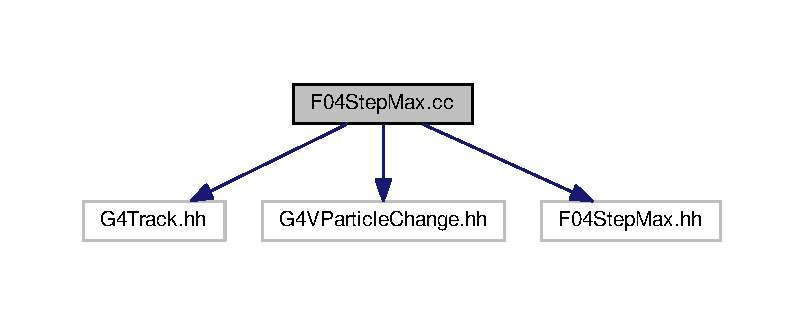
\includegraphics[width=350pt]{F04StepMax_8cc__incl}
\end{center}
\end{figure}

\hypertarget{fortran__subs_8inc}{}\section{fortran\+\_\+subs.\+inc File Reference}
\label{fortran__subs_8inc}\index{fortran\+\_\+subs.\+inc@{fortran\+\_\+subs.\+inc}}
This graph shows which files directly or indirectly include this file\+:
\nopagebreak
\begin{figure}[H]
\begin{center}
\leavevmode
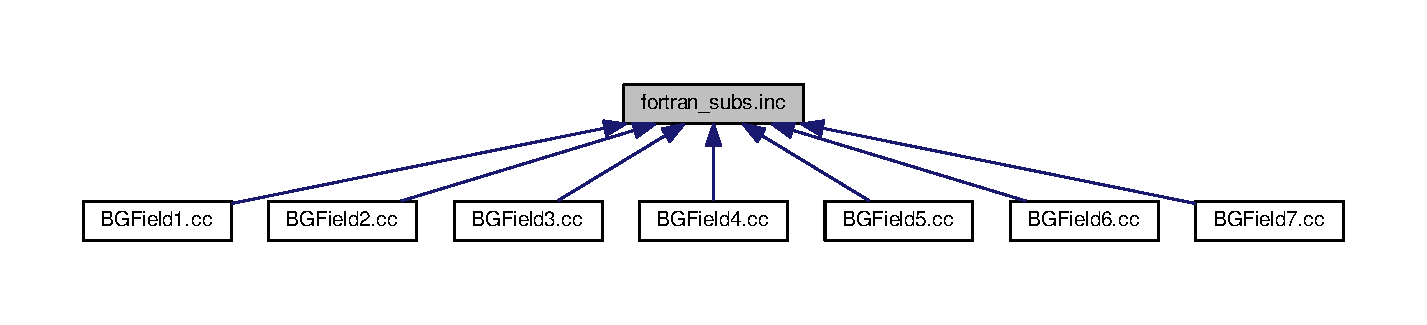
\includegraphics[width=350pt]{fortran__subs_8inc__dep__incl}
\end{center}
\end{figure}

\hypertarget{G4LindhardPartition_8cc}{}\section{G4\+Lindhard\+Partition.\+cc File Reference}
\label{G4LindhardPartition_8cc}\index{G4\+Lindhard\+Partition.\+cc@{G4\+Lindhard\+Partition.\+cc}}
{\ttfamily \#include \char`\"{}G4\+Lindhard\+Partition.\+hh\char`\"{}}\\*
{\ttfamily \#include \char`\"{}G4\+Material.\+hh\char`\"{}}\\*
{\ttfamily \#include \char`\"{}G4\+Element.\+hh\char`\"{}}\\*
{\ttfamily \#include \char`\"{}G4\+Physical\+Constants.\+hh\char`\"{}}\\*
{\ttfamily \#include \char`\"{}G4\+System\+Of\+Units.\+hh\char`\"{}}\\*
Include dependency graph for G4\+Lindhard\+Partition.\+cc\+:
\nopagebreak
\begin{figure}[H]
\begin{center}
\leavevmode
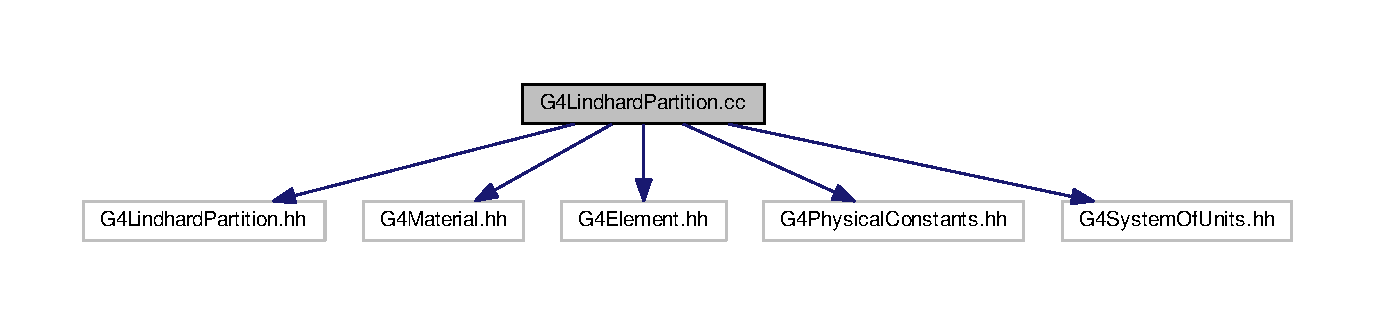
\includegraphics[width=350pt]{G4LindhardPartition_8cc__incl}
\end{center}
\end{figure}

\hypertarget{G4ScreenedNuclearRecoil_8cc}{\section{G4\-Screened\-Nuclear\-Recoil.\-cc File Reference}
\label{G4ScreenedNuclearRecoil_8cc}\index{G4\-Screened\-Nuclear\-Recoil.\-cc@{G4\-Screened\-Nuclear\-Recoil.\-cc}}
}


Implementation of the G4\-Screened\-Nuclear\-Recoil class Process for screened electromagnetic nuclear elastic scattering;.  


{\ttfamily \#include $<$stdio.\-h$>$}\\*
{\ttfamily \#include \char`\"{}globals.\-hh\char`\"{}}\\*
{\ttfamily \#include \char`\"{}G4\-Screened\-Nuclear\-Recoil.\-hh\char`\"{}}\\*
{\ttfamily \#include \char`\"{}G4\-Particle\-Types.\-hh\char`\"{}}\\*
{\ttfamily \#include \char`\"{}G4\-Particle\-Table.\-hh\char`\"{}}\\*
{\ttfamily \#include \char`\"{}G4\-V\-Particle\-Change.\-hh\char`\"{}}\\*
{\ttfamily \#include \char`\"{}G4\-Particle\-Change\-For\-Loss.\-hh\char`\"{}}\\*
{\ttfamily \#include \char`\"{}G4\-Data\-Vector.\-hh\char`\"{}}\\*
{\ttfamily \#include \char`\"{}G4\-Track.\-hh\char`\"{}}\\*
{\ttfamily \#include \char`\"{}G4\-Step.\-hh\char`\"{}}\\*
{\ttfamily \#include \char`\"{}G4\-Material.\-hh\char`\"{}}\\*
{\ttfamily \#include \char`\"{}G4\-Element.\-hh\char`\"{}}\\*
{\ttfamily \#include \char`\"{}G4\-Isotope.\-hh\char`\"{}}\\*
{\ttfamily \#include \char`\"{}G4\-Material\-Cuts\-Couple.\-hh\char`\"{}}\\*
{\ttfamily \#include \char`\"{}G4\-Element\-Vector.\-hh\char`\"{}}\\*
{\ttfamily \#include \char`\"{}G4\-Isotope\-Vector.\-hh\char`\"{}}\\*
{\ttfamily \#include \char`\"{}G4\-Em\-Process\-Sub\-Type.\-hh\char`\"{}}\\*
{\ttfamily \#include \char`\"{}G4\-Range\-Test.\-hh\char`\"{}}\\*
{\ttfamily \#include \char`\"{}G4\-Particle\-Definition.\-hh\char`\"{}}\\*
{\ttfamily \#include \char`\"{}G4\-Dynamic\-Particle.\-hh\char`\"{}}\\*
{\ttfamily \#include \char`\"{}G4\-Process\-Manager.\-hh\char`\"{}}\\*
{\ttfamily \#include \char`\"{}G4\-Stable\-Isotopes.\-hh\char`\"{}}\\*
{\ttfamily \#include \char`\"{}G4\-Lindhard\-Partition.\-hh\char`\"{}}\\*
{\ttfamily \#include \char`\"{}G4\-Physical\-Constants.\-hh\char`\"{}}\\*
{\ttfamily \#include \char`\"{}G4\-System\-Of\-Units.\-hh\char`\"{}}\\*
{\ttfamily \#include \char`\"{}Randomize.\-hh\char`\"{}}\\*
{\ttfamily \#include $<$iostream$>$}\\*
{\ttfamily \#include $<$iomanip$>$}\\*
{\ttfamily \#include \char`\"{}c2\-\_\-factory.\-hh\char`\"{}}\\*
{\ttfamily \#include $<$vector$>$}\\*
\subsection*{Typedefs}
\begin{DoxyCompactItemize}
\item 
\hypertarget{G4ScreenedNuclearRecoil_8cc_a6c336ea4b7120ec7a7ed097d8865b4b7}{typedef c2\-\_\-ptr$<$ G4double $>$ {\bfseries c2p}}\label{G4ScreenedNuclearRecoil_8cc_a6c336ea4b7120ec7a7ed097d8865b4b7}

\end{DoxyCompactItemize}
\subsection*{Functions}
\begin{DoxyCompactItemize}
\item 
\hypertarget{G4ScreenedNuclearRecoil_8cc_a38390a6f2bb8ba250affdccb1c9cc49c}{G4\-\_\-c2\-\_\-function \& {\bfseries Z\-B\-L\-Screening} (G4int z1, G4int z2, size\-\_\-t npoints, G4double r\-Max, G4double $\ast$auval)}\label{G4ScreenedNuclearRecoil_8cc_a38390a6f2bb8ba250affdccb1c9cc49c}

\item 
\hypertarget{G4ScreenedNuclearRecoil_8cc_af83b8ddfa7c0df319b4573c74bb4afd3}{G4\-\_\-c2\-\_\-function \& {\bfseries Moliere\-Screening} (G4int z1, G4int z2, size\-\_\-t npoints, G4double r\-Max, G4double $\ast$auval)}\label{G4ScreenedNuclearRecoil_8cc_af83b8ddfa7c0df319b4573c74bb4afd3}

\item 
\hypertarget{G4ScreenedNuclearRecoil_8cc_afab442d2da9f659d2c7d4b9bb1e64f5e}{G4\-\_\-c2\-\_\-function \& {\bfseries L\-J\-Screening} (G4int z1, G4int z2, size\-\_\-t npoints, G4double r\-Max, G4double $\ast$auval)}\label{G4ScreenedNuclearRecoil_8cc_afab442d2da9f659d2c7d4b9bb1e64f5e}

\item 
\hypertarget{G4ScreenedNuclearRecoil_8cc_a1e2dbe4b8a87ad052a14e6c21ad98cbf}{G4\-\_\-c2\-\_\-function \& {\bfseries L\-J\-Z\-B\-L\-Screening} (G4int z1, G4int z2, size\-\_\-t npoints, G4double r\-Max, G4double $\ast$auval)}\label{G4ScreenedNuclearRecoil_8cc_a1e2dbe4b8a87ad052a14e6c21ad98cbf}

\end{DoxyCompactItemize}


\subsection{Detailed Description}
Implementation of the G4\-Screened\-Nuclear\-Recoil class Process for screened electromagnetic nuclear elastic scattering;. See this file for more detailed in-\/body description and reference. 
\hypertarget{mitray_8cc}{}\section{mitray.\+cc File Reference}
\label{mitray_8cc}\index{mitray.\+cc@{mitray.\+cc}}
{\ttfamily \#include $<$f2c.\+h$>$}\\*
Include dependency graph for mitray.\+cc\+:
\nopagebreak
\begin{figure}[H]
\begin{center}
\leavevmode
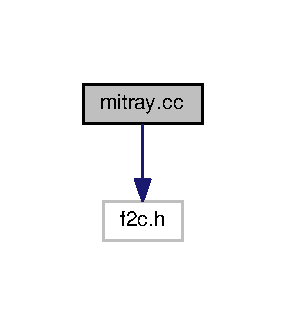
\includegraphics[width=137pt]{mitray_8cc__incl}
\end{center}
\end{figure}
\subsection*{Macros}
\begin{DoxyCompactItemize}
\item 
\#define \hyperlink{mitray_8cc_a9e8f83ecadfaef78a89880c2f1ce4d0b}{mitray\+\_\+dipo\+\_\+\+\_\+1}~\hyperlink{mitray_8cc_a8c1f30c771bb5cdf549960cb4e72a941}{mitray\+\_\+dipo\+\_\+\+\_\+}
\item 
\#define \hyperlink{mitray_8cc_a28e7035bd99e147a47ea6838cef13528}{mitray24\+\_\+1}~\hyperlink{mitray_8cc_a579878e78f4a54716669008d43fad7ae}{mitray24\+\_\+}
\item 
\#define \hyperlink{mitray_8cc_a9dc5985c74c9095394c4dc6ec9030365}{mitray10\+\_\+1}~(\hyperlink{mitray_8cc_acdd8181096f6b6dd2f811f4b52c7bd74}{mitray10\+\_\+.\+\_\+1})
\item 
\#define \hyperlink{mitray_8cc_a1308a38a194422b36da7903024d794b5}{mitray10\+\_\+2}~(\hyperlink{mitray_8cc_a941388ee8d1a88377f8a17fd847ba9e5}{mitray10\+\_\+.\+\_\+2})
\item 
\#define \hyperlink{mitray_8cc_a892e0f259b620f45977f5bbb90155ba7}{mitray20\+\_\+1}~(\hyperlink{mitray_8cc_acdd8181096f6b6dd2f811f4b52c7bd74}{mitray20\+\_\+.\+\_\+1})
\item 
\#define \hyperlink{mitray_8cc_aaf65e5553573a36d98fe9be7bc738342}{mitray20\+\_\+2}~(\hyperlink{mitray_8cc_a941388ee8d1a88377f8a17fd847ba9e5}{mitray20\+\_\+.\+\_\+2})
\item 
\#define \hyperlink{mitray_8cc_a84489423716883b6e513f4ad164ce1c7}{mitray21\+\_\+1}~\hyperlink{mitray_8cc_a05f57450ae827c9b5ab0788dd6a82c1b}{mitray21\+\_\+}
\item 
\#define \hyperlink{mitray_8cc_a8cdca1fddc1016e3a0d8b453c6905829}{mitray22\+\_\+1}~(\hyperlink{mitray_8cc_acdd8181096f6b6dd2f811f4b52c7bd74}{mitray22\+\_\+.\+\_\+1})
\item 
\#define \hyperlink{mitray_8cc_a58cb955f31a7f4c8dd89ae38ba1c2dd1}{mitray22\+\_\+2}~(\hyperlink{mitray_8cc_a941388ee8d1a88377f8a17fd847ba9e5}{mitray22\+\_\+.\+\_\+2})
\item 
\#define \hyperlink{mitray_8cc_a22f3528c02dc4a34855204546e970816}{mitray23\+\_\+1}~\hyperlink{mitray_8cc_afefc0d7e0e2f5ace369fcb809bea50c4}{mitray23\+\_\+}
\item 
\#define \hyperlink{mitray_8cc_abb31a8e37a6bc2d9210b50f1678434ab}{mitray25\+\_\+1}~(\hyperlink{mitray_8cc_acdd8181096f6b6dd2f811f4b52c7bd74}{mitray25\+\_\+.\+\_\+1})
\item 
\#define \hyperlink{mitray_8cc_a562557c27741020e09dba1607fc038dd}{mitray25\+\_\+2}~(\hyperlink{mitray_8cc_a941388ee8d1a88377f8a17fd847ba9e5}{mitray25\+\_\+.\+\_\+2})
\item 
\#define \hyperlink{mitray_8cc_a00e4400af42cd1ac0b4ab3762ba221e3}{mitray\+\_\+axes\+\_\+\+\_\+1}~\hyperlink{mitray_8cc_a4f7e24c5850a2d1df6e63b1b1290cd96}{mitray\+\_\+axes\+\_\+\+\_\+}
\item 
\#define \hyperlink{mitray_8cc_a3fbaad4622a203c44cfe9d44b98626c8}{mitray\+\_\+bounds\+\_\+\+\_\+1}~\hyperlink{mitray_8cc_ab619a86d3c8dd24516408c7c15279a08}{mitray\+\_\+bounds\+\_\+\+\_\+}
\item 
\#define \hyperlink{mitray_8cc_a730b12cafdc4aa9fbbfde11fe48c00f0}{gcflag\+\_\+1}~\hyperlink{mitray_8cc_a8e2354adddb9316d29a6dfde0069e79c}{gcflag\+\_\+}
\item 
\#define \hyperlink{mitray_8cc_a38f3eae11565315923507968e34470b0}{gcflax\+\_\+1}~\hyperlink{mitray_8cc_a64bfa183f86af319dfa4ccae5a13cbdb}{gcflax\+\_\+}
\item 
\#define \hyperlink{mitray_8cc_ad75de819cb0993812f8e48efdb8fc495}{gcunit\+\_\+1}~\hyperlink{mitray_8cc_a511fd49332d1fb71f0150048ab79e355}{gcunit\+\_\+}
\item 
\#define \hyperlink{mitray_8cc_afe66a8c9c62ed6b8392453bd1c91d67b}{gcmail\+\_\+1}~\hyperlink{mitray_8cc_a284a3a869f35000eafa74dd8f82fc90e}{gcmail\+\_\+}
\item 
\#define \hyperlink{mitray_8cc_a13375d8e677747a0fcf4001e4eb69e0a}{mitray\+\_\+diag\+\_\+\+\_\+1}~\hyperlink{mitray_8cc_aa11f84cade6df03871fb2a1aad89e062}{mitray\+\_\+diag\+\_\+\+\_\+}
\item 
\#define \hyperlink{mitray_8cc_a0e5637b3a2a7e6f95057b95a4e1c314d}{diag\+\_\+1}~\hyperlink{mitray_8cc_afd82ad19234f568cb23cd98b14550577}{diag\+\_\+}
\item 
\#define \hyperlink{mitray_8cc_ae57b9e50d877dd78326ef5f848602ef1}{mitrayblsdip\+\_\+1}~\hyperlink{mitray_8cc_a6626e97b1a2dd5f002f4615f1be031e0}{mitrayblsdip\+\_\+}
\item 
\#define \hyperlink{mitray_8cc_a34ec230608c6bf79cec941d7a0c48f1e}{mitray26\+\_\+1}~\hyperlink{mitray_8cc_a32a9d12dea99297f76e99158f6fa2af5}{mitray26\+\_\+}
\item 
\#define \hyperlink{mitray_8cc_a699892b15b26db6d7659ec4907605186}{mitray11\+\_\+1}~\hyperlink{mitray_8cc_a438be24b8b9055b569629ebc4afbb58c}{mitray11\+\_\+}
\item 
\#define \hyperlink{mitray_8cc_a634b52487a2f67b2511757c7cd499b1f}{mitray\+\_\+edipo\+\_\+\+\_\+1}~\hyperlink{mitray_8cc_af2f29f245c80b4b3b7b20b63d4e2a751}{mitray\+\_\+edipo\+\_\+\+\_\+}
\item 
\#define \hyperlink{mitray_8cc_ae75232d8b543414d710c8d35be60f8f3}{mitray5\+\_\+1}~\hyperlink{mitray_8cc_a114c95ec3e802b744f0987db19b5f737}{mitray5\+\_\+}
\item 
\#define \hyperlink{mitray_8cc_af1618c2933ef2c517fbeff39e34a2b46}{mitray90\+\_\+1}~\hyperlink{mitray_8cc_a910b0e7398b29dfeef3b52c0d40601ba}{mitray90\+\_\+}
\item 
\#define \hyperlink{mitray_8cc_a454d7016695157a68f25fff1f1c29227}{mitray91\+\_\+1}~\hyperlink{mitray_8cc_a9c75de125228cd6fbba6c909bf79491d}{mitray91\+\_\+}
\item 
\#define \hyperlink{mitray_8cc_a5b2aaeaede377c5f2e8f1c53749e28c4}{mitray92\+\_\+1}~\hyperlink{mitray_8cc_a9deb0bccabea6f7ae6e1dd6b3c899eb6}{mitray92\+\_\+}
\item 
\#define \hyperlink{mitray_8cc_a6ecd623017fa06118721ec886267bf93}{mitray93\+\_\+1}~\hyperlink{mitray_8cc_ac1c1e96612517f1e08b7d05b6cd7b7ef}{mitray93\+\_\+}
\item 
\#define \hyperlink{mitray_8cc_a71179bd82c74589bb4e34a77920f1f6e}{mitray30\+\_\+1}~\hyperlink{mitray_8cc_a56278942f2bf1f640fa020fe9527c8e4}{mitray30\+\_\+}
\item 
\#define \hyperlink{mitray_8cc_a73dcb1fd9d9889bcbcf1c726e6f37483}{mitray31\+\_\+1}~\hyperlink{mitray_8cc_a3b40001ffe99cb01bf6f2ba35e1e1984}{mitray31\+\_\+}
\end{DoxyCompactItemize}
\subsection*{Functions}
\begin{DoxyCompactItemize}
\item 
int \hyperlink{mitray_8cc_a5e59c7389866e881a27d293194e99a8f}{mitray\+\_\+dipo\+\_\+atob\+\_\+\+\_\+} (doublereal $\ast$\hyperlink{mitray_8cc_adc5cbb0ed87c4256ed823b5c03c48c08}{xa}, doublereal $\ast$\hyperlink{mitray_8cc_ac9005acb2a7fcd170dc241fbead0d78d}{ya}, doublereal $\ast$\hyperlink{mitray_8cc_af8dd9890ff2807fbc890e1a41577fbcd}{za}, doublereal $\ast$\hyperlink{mitray_8cc_a7ab9deb8ae4501fcbe7cd3ecfa738062}{xb}, doublereal $\ast$\hyperlink{mitray_8cc_a4debd825afd301e44789121a65651eeb}{yb}, doublereal $\ast$\hyperlink{mitray_8cc_a0b50f025ccf7b3b83c86bb76fbc1d61c}{zb})
\item 
int \hyperlink{mitray_8cc_a01670be7489ba68ed94c12be6e20f749}{mitray\+\_\+dipo\+\_\+btoc\+\_\+\+\_\+} (doublereal $\ast$\hyperlink{mitray_8cc_a7ab9deb8ae4501fcbe7cd3ecfa738062}{xb}, doublereal $\ast$\hyperlink{mitray_8cc_a4debd825afd301e44789121a65651eeb}{yb}, doublereal $\ast$\hyperlink{mitray_8cc_a0b50f025ccf7b3b83c86bb76fbc1d61c}{zb}, doublereal $\ast$\hyperlink{mitray_8cc_af4db73efb12ca5dec7783d898617ad4c}{xc}, doublereal $\ast$\hyperlink{mitray_8cc_a0c86d304d51dd763531b7988667788b0}{yc}, doublereal $\ast$\hyperlink{mitray_8cc_a5adb2b50408db7bedc679a420440ea7b}{zc})
\item 
int \hyperlink{mitray_8cc_a186998df5373a1577d298fd05d6f73b5}{mitray\+\_\+dipo\+\_\+bbtoba\+\_\+\+\_\+} (doublereal $\ast$bxb, doublereal $\ast$byb, doublereal $\ast$bzb, doublereal $\ast$bxa, doublereal $\ast$bya, doublereal $\ast$bza)
\item 
int \hyperlink{mitray_8cc_a26ec78b9409543a16e7d0211fea0b487}{mitray\+\_\+dipo\+\_\+bctobb\+\_\+\+\_\+} (doublereal $\ast$bxc, doublereal $\ast$byc, doublereal $\ast$bzc, doublereal $\ast$bxb, doublereal $\ast$byb, doublereal $\ast$bzb)
\item 
int \hyperlink{mitray_8cc_a8763ad237663f55a27c683601eba1257}{mitray\+\_\+dipole\+\_\+\+\_\+} (doublereal $\ast$data, doublereal $\ast$xpos, doublereal $\ast$bfld)
\item 
int \hyperlink{mitray_8cc_aac77a7def3509d267e595814d340fe33}{mitray\+\_\+bdip\+\_\+\+\_\+} ()
\item 
int \hyperlink{mitray_8cc_a58b0762ef3e8e777088c4dc9f5fb6202}{mitray\+\_\+bdpp\+\_\+\+\_\+0\+\_\+} (int n\+\_\+\+\_\+, doublereal $\ast$bfld, doublereal $\ast$z\+\_\+\+\_\+, doublereal $\ast$x, integer $\ast$i\+\_\+\+\_\+, integer $\ast$j)
\item 
int \hyperlink{mitray_8cc_a88c6487e0dddcb6162bbf4ba7c5f2a95}{mitray\+\_\+bdpp\+\_\+\+\_\+} (doublereal $\ast$bfld, doublereal $\ast$z\+\_\+\+\_\+, doublereal $\ast$x)
\item 
int \hyperlink{mitray_8cc_a679e5a2d58d8f97bb98f3ca835ec1a36}{mitray\+\_\+bdppx\+\_\+\+\_\+} (doublereal $\ast$bfld, integer $\ast$i\+\_\+\+\_\+, integer $\ast$j)
\item 
int \hyperlink{mitray_8cc_a013ade5f554fe29df6016200b7c6e932}{mitray\+\_\+ndip\+\_\+\+\_\+} ()
\item 
int \hyperlink{mitray_8cc_a61683028e0262fa0ab2f350cec04f7f7}{mitray\+\_\+ndpp\+\_\+\+\_\+0\+\_\+} (int n\+\_\+\+\_\+, doublereal $\ast$bfld, doublereal $\ast$z\+\_\+\+\_\+, doublereal $\ast$x, doublereal $\ast$dr, integer $\ast$i\+\_\+\+\_\+, integer $\ast$j)
\item 
int \hyperlink{mitray_8cc_a26a439356649e8f059e6caa564e8e4e5}{mitray\+\_\+ndpp\+\_\+\+\_\+} (doublereal $\ast$bfld, doublereal $\ast$z\+\_\+\+\_\+, doublereal $\ast$x, doublereal $\ast$dr)
\item 
int \hyperlink{mitray_8cc_a6f76129495df2c49357cdc897bfc5558}{mitray\+\_\+ndppx\+\_\+\+\_\+} (doublereal $\ast$bfld, integer $\ast$i\+\_\+\+\_\+, integer $\ast$j, doublereal $\ast$dr)
\item 
int \hyperlink{mitray_8cc_a4068019379169ffb6be3dea7c7a1a74d}{mitray\+\_\+bpretz\+\_\+\+\_\+} ()
\item 
int \hyperlink{mitray_8cc_ae6d45cfe222d61d5ef6723f87d2bdd74}{mitray\+\_\+sdip\+\_\+\+\_\+0\+\_\+} (int n\+\_\+\+\_\+, doublereal $\ast$x, doublereal $\ast$z\+\_\+\+\_\+, integer $\ast$\hyperlink{mitray_8cc_a8c41adfb7355eb461d99936e02b9e859}{iz}, integer $\ast$jx)
\item 
int \hyperlink{mitray_8cc_ad2241953a2d2d1eb7c8ffbbc8537166f}{mitray\+\_\+sdip\+\_\+\+\_\+} (doublereal $\ast$x, doublereal $\ast$z\+\_\+\+\_\+)
\item 
int \hyperlink{mitray_8cc_ac37f508d357141cd6ed103916150410f}{mitray\+\_\+sij\+\_\+\+\_\+} (integer $\ast$\hyperlink{mitray_8cc_a8c41adfb7355eb461d99936e02b9e859}{iz}, integer $\ast$jx)
\item 
doublereal \hyperlink{mitray_8cc_a846e2adbf8b2f92a5272dfd6fe4a10f3}{xmitray\+\_\+zefb\+\_\+\+\_\+} (doublereal $\ast$xp)
\item 
doublereal \hyperlink{mitray_8cc_afad96f6767e7c37d9fa9323be2e9c5e3}{xmitray\+\_\+dzdx\+\_\+\+\_\+} (doublereal $\ast$xp)
\item 
doublereal \hyperlink{mitray_8cc_adddef6c13863b2b6e99eea7260c85970}{xmitray\+\_\+dzdx2\+\_\+\+\_\+} (doublereal $\ast$xp)
\item 
int \hyperlink{mitray_8cc_aad6464ccc06c8e3a4c0bcde464c39884}{mitray\+\_\+bdmp\+\_\+\+\_\+} (doublereal $\ast$bzz, doublereal $\ast$z\+\_\+\+\_\+, doublereal $\ast$x)
\item 
int \hyperlink{mitray_8cc_a72b35f12c5d7b0b4167908d005ed78db}{mitray\+\_\+edipol\+\_\+\+\_\+} (doublereal $\ast$data, doublereal $\ast$xpos, doublereal $\ast$efld)
\item 
int \hyperlink{mitray_8cc_a7ecb253c26ba3db2b07db22bd892930f}{mitray\+\_\+edip\+\_\+\+\_\+} ()
\item 
int \hyperlink{mitray_8cc_ab6fdca410afb6aa53ea295580a4fcc61}{mitray\+\_\+edpp\+\_\+\+\_\+} (doublereal $\ast$\hyperlink{mitray_8cc_a67e960748c43e0af88b251d68d1aa9d1}{d\+\_\+\+\_\+}, doublereal $\ast$\hyperlink{mitray_8cc_a8f241202b21e550b9dd25d7692bd38df}{s}, doublereal $\ast$re, doublereal $\ast$g1, doublereal $\ast$g2, doublereal $\ast$g3, doublereal $\ast$g4, doublereal $\ast$g5, doublereal $\ast$g6)
\item 
int \hyperlink{mitray_8cc_a23664744fbfe1033f743f5f9d465351c}{mitray\+\_\+edip\+\_\+ectoea\+\_\+\+\_\+} (doublereal $\ast$exc, doublereal $\ast$eyc, doublereal $\ast$ezc, doublereal $\ast$exa, doublereal $\ast$eya, doublereal $\ast$eza)
\item 
int \hyperlink{mitray_8cc_ac4e75918a850bc130d44843074a5daa3}{mitray\+\_\+poles\+\_\+\+\_\+} (doublereal $\ast$data, doublereal $\ast$xpos, doublereal $\ast$bfld)
\item 
int \hyperlink{mitray_8cc_a0bee4bfdaaab9ddec7ce54387fa912a7}{mitray\+\_\+bpoles\+\_\+\+\_\+} ()
\item 
int \hyperlink{mitray_8cc_afcd6ee409614b786e9f63ca0ce7071ac}{mitray\+\_\+bpls\+\_\+\+\_\+} (integer $\ast$igp, doublereal $\ast$\hyperlink{mitray_8cc_a67e960748c43e0af88b251d68d1aa9d1}{d\+\_\+\+\_\+}, doublereal $\ast$\hyperlink{mitray_8cc_a8f241202b21e550b9dd25d7692bd38df}{s}, doublereal $\ast$re, doublereal $\ast$g1, doublereal $\ast$g2, doublereal $\ast$g3, doublereal $\ast$g4, doublereal $\ast$g5, doublereal $\ast$g6)
\item 
int \hyperlink{mitray_8cc_aaae0e43999a2aa0fcdbb95da91b0b0c7}{mitray\+\_\+sasp\+\_\+\+\_\+} (doublereal $\ast$data, doublereal $\ast$xpos, doublereal $\ast$bfld)
\item 
int \hyperlink{mitray_8cc_a1dd6073236d4ee5ba605c67e50a4ca5f}{mitray\+\_\+saspratio\+\_\+\+\_\+} (doublereal $\ast$bmeas0, doublereal $\ast$\hyperlink{mitray_8cc_adc5cbb0ed87c4256ed823b5c03c48c08}{xa}, doublereal $\ast$ratio)
\item 
int \hyperlink{mitray_8cc_ab0123cace3b71e951b3dc56825cb11cc}{mitray\+\_\+solnd\+\_\+\+\_\+} (doublereal $\ast$data, doublereal $\ast$xpos, doublereal $\ast$bfld)
\item 
int \hyperlink{mitray_8cc_a9934206b20e8a92583ca9132cdc7200c}{mitray\+\_\+bsol\+\_\+\+\_\+} ()
\item 
int \hyperlink{mitray_8cc_aaebeef5eef35af4e7f94482a1ada5219}{mitray\+\_\+fb01ad\+\_\+\+\_\+} (doublereal $\ast$c\+\_\+\+\_\+, doublereal $\ast$vk, doublereal $\ast$ve)
\item 
int \hyperlink{mitray_8cc_a65ce2094441a1be8ccea237d584cb4b7}{mitray\+\_\+fb02ad\+\_\+\+\_\+} (doublereal $\ast$caysq, doublereal $\ast$sinp, doublereal $\ast$cosp, doublereal $\ast$e, doublereal $\ast$f)
\item 
int \hyperlink{mitray_8cc_a4f95c0d166f0b2d83d0bd7b9143276b5}{mitray\+\_\+fb03ad\+\_\+\+\_\+} (doublereal $\ast$gn, doublereal $\ast$caca, doublereal $\ast$p)
\item 
int \hyperlink{mitray_8cc_a427270d43ad148138af5df2c898ba32e}{mitray\+\_\+zone\+\_\+\+\_\+} (doublereal $\ast$\hyperlink{mitray_8cc_a0b50f025ccf7b3b83c86bb76fbc1d61c}{zb}, doublereal $\ast$\hyperlink{mitray_8cc_a5adb2b50408db7bedc679a420440ea7b}{zc}, doublereal $\ast$z11, doublereal $\ast$z12, doublereal $\ast$z21, doublereal $\ast$z22, integer $\ast$izone)
\end{DoxyCompactItemize}
\subsection*{Variables}
\begin{DoxyCompactItemize}
\item 
\begin{tabbing}
xx\=xx\=xx\=xx\=xx\=xx\=xx\=xx\=xx\=\kill
struct \{\\
\>doublereal \hyperlink{mitray_8cc_a2741c8c93c73b15dd2be5092b62aac8c}{a}\\
\>doublereal \hyperlink{mitray_8cc_a32dd5c98fee19eac3d7d7737e3482023}{b}\\
\>doublereal \hyperlink{mitray_8cc_ac848511d5e241911e98fce8f1991d830}{phi}\\
\>doublereal \hyperlink{mitray_8cc_a9d0f27da38432b15fc30f2714b642ee7}{alpha}\\
\>doublereal \hyperlink{mitray_8cc_a0f4d8a67bb39acc583704de120c23b36}{beta}\\
\>doublereal \hyperlink{mitray_8cc_a928f6f1254049fccebc29997796bcd5f}{xcr1}\\
\>doublereal \hyperlink{mitray_8cc_ace84d45cf82e3368517c5f36a7ec5f1d}{xcr2}\\
\} \hyperlink{mitray_8cc_a8c1f30c771bb5cdf549960cb4e72a941}{mitray\_dipo\_\_}\\

\end{tabbing}\item 
\begin{tabbing}
xx\=xx\=xx\=xx\=xx\=xx\=xx\=xx\=xx\=\kill
struct \{\\
\>doublereal \hyperlink{mitray_8cc_a78d809cec9b014137fff9596f4559598}{rb}\\
\>doublereal \hyperlink{mitray_8cc_a14470c2d4bca9476f55d7d8b572c9bae}{xc\_offset\_\_}\\
\>doublereal \hyperlink{mitray_8cc_a4a123f4cb09f631ddc8ee6b9bacb4d41}{zc\_offset\_\_}\\
\} \hyperlink{mitray_8cc_a579878e78f4a54716669008d43fad7ae}{mitray24\_}\\

\end{tabbing}\item 
\begin{tabbing}
xx\=xx\=xx\=xx\=xx\=xx\=xx\=xx\=xx\=\kill
union \{\\
\>struct \{\\
\>\>doublereal \hyperlink{mitray_8cc_a64f5f0d4d7d07759a3a2743ec0aa27e2}{bx}\\
\>\>doublereal \hyperlink{mitray_8cc_afdc40421cd017339e8740c3f09156ab3}{by}\\
\>\>doublereal \hyperlink{mitray_8cc_a144d519c628768b23c549dcfc7b0ec3f}{bz}\\
\>\>doublereal \hyperlink{mitray_8cc_a4a74e9ca460675a82e0ee25b5ba2eaa2}{k}\\
\>\>doublereal \hyperlink{mitray_8cc_ada670964b6e4104b69d3a088118bbdf6}{tc} \mbox{[}6\mbox{]}\\
\>\>doublereal \hyperlink{mitray_8cc_a4ce5911207220f34cb2a92f97be46b1c}{dtc} \mbox{[}6\mbox{]}\\
\>\} \hyperlink{mitray_8cc_acdd8181096f6b6dd2f811f4b52c7bd74}{\_1}\\
\>struct \{\\
\>\>doublereal \hyperlink{mitray_8cc_a64f5f0d4d7d07759a3a2743ec0aa27e2}{bx}\\
\>\>doublereal \hyperlink{mitray_8cc_afdc40421cd017339e8740c3f09156ab3}{by}\\
\>\>doublereal \hyperlink{mitray_8cc_a144d519c628768b23c549dcfc7b0ec3f}{bz}\\
\>\>doublereal \hyperlink{mitray_8cc_ada670964b6e4104b69d3a088118bbdf6}{tc} \mbox{[}6\mbox{]}\\
\>\>doublereal \hyperlink{mitray_8cc_a4ce5911207220f34cb2a92f97be46b1c}{dtc} \mbox{[}6\mbox{]}\\
\>\} \hyperlink{mitray_8cc_a941388ee8d1a88377f8a17fd847ba9e5}{\_2}\\
\} \hyperlink{mitray_8cc_a6ac553da330fc5b6a752dc506f2b5e80}{mitray10\_}\\

\end{tabbing}\item 
\begin{tabbing}
xx\=xx\=xx\=xx\=xx\=xx\=xx\=xx\=xx\=\kill
union \{\\
\>struct \{\\
\>\>doublereal \hyperlink{mitray_8cc_ae8418c9cf569b83acfc6b386cf5f157b}{ndx}\\
\>\>doublereal \hyperlink{mitray_8cc_a2aa9b53defe42bc770ad6b5b2ec6516f}{bet1}\\
\>\>doublereal \hyperlink{mitray_8cc_a3b5364373d9df1c779e28b9903d1bc6e}{gama}\\
\>\>doublereal \hyperlink{mitray_8cc_a3ba3670064863d640e2e3be166a61362}{delt}\\
\>\} \hyperlink{mitray_8cc_acdd8181096f6b6dd2f811f4b52c7bd74}{\_1}\\
\>struct \{\\
\>\>doublereal \hyperlink{mitray_8cc_ab45e18c6c6d23137daa8b056382c470b}{ec2}\\
\>\>doublereal \hyperlink{mitray_8cc_a227e880a422ebe5ecede260e9ddef266}{ec4}\\
\>\>doublereal \hyperlink{mitray_8cc_ac1b648f83d620109f08ceee9545855d0}{we}\\
\>\>doublereal \hyperlink{mitray_8cc_a939c8da6e0e485de8aa955a711925d50}{wc}\\
\>\} \hyperlink{mitray_8cc_a941388ee8d1a88377f8a17fd847ba9e5}{\_2}\\
\} \hyperlink{mitray_8cc_ab560691bea78eab2ca025605d590d94c}{mitray20\_}\\

\end{tabbing}\item 
\begin{tabbing}
xx\=xx\=xx\=xx\=xx\=xx\=xx\=xx\=xx\=\kill
struct \{\\
\>doublereal \hyperlink{mitray_8cc_a7e40ffb68c5bebe1902a945ce01fdd09}{rca}\\
\>doublereal \hyperlink{mitray_8cc_a32410d05294d3fc555551ad0724b5eb1}{dels}\\
\>doublereal \hyperlink{mitray_8cc_a56754ea31f91ce7907a6697179da2ad2}{br}\\
\>doublereal \hyperlink{mitray_8cc_aab893faf378002357035384178222d26}{s2}\\
\>doublereal \hyperlink{mitray_8cc_aed05f0ccefbd4e0120c920428789b9f3}{s3}\\
\>doublereal \hyperlink{mitray_8cc_a1e1a7e5f17118f4bfe5805d6426a11cc}{s4}\\
\>doublereal \hyperlink{mitray_8cc_a38fb30422676b2f23603c507d61f3419}{s5}\\
\>doublereal \hyperlink{mitray_8cc_ac59491a7d92534a9e7883bbead435c9a}{s6}\\
\>doublereal \hyperlink{mitray_8cc_a28e9625b04051cacf62e8c162273b97b}{s7}\\
\>doublereal \hyperlink{mitray_8cc_ae613556f83262c872ab0d37dcbf1e585}{s8}\\
\} \hyperlink{mitray_8cc_a05f57450ae827c9b5ab0788dd6a82c1b}{mitray21\_}\\

\end{tabbing}\item 
\begin{tabbing}
xx\=xx\=xx\=xx\=xx\=xx\=xx\=xx\=xx\=\kill
union \{\\
\>struct \{\\
\>\>doublereal \hyperlink{mitray_8cc_a67e960748c43e0af88b251d68d1aa9d1}{d\_\_}\\
\>\>doublereal \hyperlink{mitray_8cc_aa3ff0f70409c05e4faf468845b6af783}{dg}\\
\>\>doublereal \hyperlink{mitray_8cc_a8f241202b21e550b9dd25d7692bd38df}{s}\\
\>\>doublereal \hyperlink{mitray_8cc_a163fc56161730a9b50b69980756b87f6}{bf}\\
\>\>doublereal \hyperlink{mitray_8cc_ad59db50b6be8f97566cfa77e50c35619}{bt}\\
\>\>doublereal \hyperlink{mitray_8cc_a7c50114013d785fb14c99b82d219fbd3}{wdip}\\
\>\} \hyperlink{mitray_8cc_acdd8181096f6b6dd2f811f4b52c7bd74}{\_1}\\
\>struct \{\\
\>\>doublereal \hyperlink{mitray_8cc_a67e960748c43e0af88b251d68d1aa9d1}{d\_\_}\\
\>\>doublereal \hyperlink{mitray_8cc_aa3ff0f70409c05e4faf468845b6af783}{dg}\\
\>\>doublereal \hyperlink{mitray_8cc_a8f241202b21e550b9dd25d7692bd38df}{s}\\
\>\>doublereal \hyperlink{mitray_8cc_adda353887375edda51958d50160a9dff}{ef}\\
\>\>doublereal \hyperlink{mitray_8cc_af1dae735c63fbadf97605e948ca483d9}{et}\\
\>\>doublereal \hyperlink{mitray_8cc_a3ef132c776f5a8fe32034839ac727b8d}{dum}\\
\>\} \hyperlink{mitray_8cc_a941388ee8d1a88377f8a17fd847ba9e5}{\_2}\\
\} \hyperlink{mitray_8cc_a6a060b56f632f86a170f05b4b76939b7}{mitray22\_}\\

\end{tabbing}\item 
\begin{tabbing}
xx\=xx\=xx\=xx\=xx\=xx\=xx\=xx\=xx\=\kill
struct \{\\
\>doublereal \hyperlink{mitray_8cc_a035c9b21735af6423b417c1836fc55dc}{c0}\\
\>doublereal \hyperlink{mitray_8cc_ad1e974583ab5d8a5c6f23ba636ad61f9}{c1}\\
\>doublereal \hyperlink{mitray_8cc_a9e80dc05648874bab314be17f6f44ac6}{c2}\\
\>doublereal \hyperlink{mitray_8cc_a273f5014a58a4f8f6c3279b981d6c4c3}{c3}\\
\>doublereal \hyperlink{mitray_8cc_ae516f45611a113a3eb796b5dcf5ee8e1}{c4}\\
\>doublereal \hyperlink{mitray_8cc_a8b11b259e9bbb72719718fc0c5767d97}{c5}\\
\} \hyperlink{mitray_8cc_afefc0d7e0e2f5ace369fcb809bea50c4}{mitray23\_}\\

\end{tabbing}\item 
\begin{tabbing}
xx\=xx\=xx\=xx\=xx\=xx\=xx\=xx\=xx\=\kill
union \{\\
\>struct \{\\
\>\>integer \hyperlink{mitray_8cc_a9d35985edcd8c14b69ce535a682610c8}{in}\\
\>\>integer \hyperlink{mitray_8cc_af72f0675460479dad4bb15582c23c4a7}{mtyp}\\
\>\>integer \hyperlink{mitray_8cc_a9d7c2577bc05eb8563a8f62f6bda320d}{nsrf}\\
\>\>integer \hyperlink{mitray_8cc_a3b39cf1429a05d86c20508aa252b87bb}{imap}\\
\>\>integer \hyperlink{mitray_8cc_a79fbdfd6d18963a5b89c61facf5afdfc}{ir}\\
\>\} \hyperlink{mitray_8cc_acdd8181096f6b6dd2f811f4b52c7bd74}{\_1}\\
\>struct \{\\
\>\>integer \hyperlink{mitray_8cc_a9d35985edcd8c14b69ce535a682610c8}{in}\\
\>\>integer \hyperlink{mitray_8cc_af72f0675460479dad4bb15582c23c4a7}{mtyp}\\
\>\>integer \hyperlink{mitray_8cc_a9d7c2577bc05eb8563a8f62f6bda320d}{nsrf}\\
\>\>integer \hyperlink{mitray_8cc_ac09634fb0b53cd4a9d3da2be311d1316}{idum1}\\
\>\>integer \hyperlink{mitray_8cc_a7fa1b8f7a55d22f3cbb97fcc8a93540f}{idum2}\\
\>\} \hyperlink{mitray_8cc_a941388ee8d1a88377f8a17fd847ba9e5}{\_2}\\
\} \hyperlink{mitray_8cc_a1b8e79846999293e920718d79a3dabb5}{mitray25\_}\\

\end{tabbing}\item 
\begin{tabbing}
xx\=xx\=xx\=xx\=xx\=xx\=xx\=xx\=xx\=\kill
struct \{\\
\>doublereal \hyperlink{mitray_8cc_adc5cbb0ed87c4256ed823b5c03c48c08}{xa}\\
\>doublereal \hyperlink{mitray_8cc_ac9005acb2a7fcd170dc241fbead0d78d}{ya}\\
\>doublereal \hyperlink{mitray_8cc_af8dd9890ff2807fbc890e1a41577fbcd}{za}\\
\>doublereal \hyperlink{mitray_8cc_a7ab9deb8ae4501fcbe7cd3ecfa738062}{xb}\\
\>doublereal \hyperlink{mitray_8cc_a4debd825afd301e44789121a65651eeb}{yb}\\
\>doublereal \hyperlink{mitray_8cc_a0b50f025ccf7b3b83c86bb76fbc1d61c}{zb}\\
\>doublereal \hyperlink{mitray_8cc_af4db73efb12ca5dec7783d898617ad4c}{xc}\\
\>doublereal \hyperlink{mitray_8cc_a0c86d304d51dd763531b7988667788b0}{yc}\\
\>doublereal \hyperlink{mitray_8cc_a5adb2b50408db7bedc679a420440ea7b}{zc}\\
\} \hyperlink{mitray_8cc_a4f7e24c5850a2d1df6e63b1b1290cd96}{mitray\_axes\_\_}\\

\end{tabbing}\item 
\begin{tabbing}
xx\=xx\=xx\=xx\=xx\=xx\=xx\=xx\=xx\=\kill
struct \{\\
\>doublereal \hyperlink{mitray_8cc_a786d9b42c471f31d3d17653f296f9848}{xbmin}\\
\>doublereal \hyperlink{mitray_8cc_ac80f0a2d79fa82243c6ab434a0d08a7d}{xbmax}\\
\>doublereal \hyperlink{mitray_8cc_aacf7ede97b766c097894155a2573fbcd}{xcmin}\\
\>doublereal \hyperlink{mitray_8cc_a2c6c98b10e9a429b25c20746253f113a}{xcmax}\\
\} \hyperlink{mitray_8cc_ab619a86d3c8dd24516408c7c15279a08}{mitray\_bounds\_\_}\\

\end{tabbing}\item 
\begin{tabbing}
xx\=xx\=xx\=xx\=xx\=xx\=xx\=xx\=xx\=\kill
struct \{\\
\>integer \hyperlink{mitray_8cc_a9bf6766836180bf4aab09c5094e3a430}{idebug}\\
\>integer \hyperlink{mitray_8cc_a533c22cdd5571db96d51e2a69a80e8dd}{idemin}\\
\>integer \hyperlink{mitray_8cc_a2e4d8b47d1696da98aa931b2eac6153f}{idemax}\\
\>integer \hyperlink{mitray_8cc_a94cf2780882d6285fce053dd3a6100eb}{itest}\\
\>integer \hyperlink{mitray_8cc_a858cfe9f313da8b51f13ccfab772ded7}{idrun}\\
\>integer \hyperlink{mitray_8cc_a5083347df89778b06e07b871b1539326}{idevt}\\
\>integer \hyperlink{mitray_8cc_a4fe421de428e1cf68b3956860d34af54}{ieorun}\\
\>integer \hyperlink{mitray_8cc_a875b8b80f14e31d9935f5621c3616176}{ieotri}\\
\>integer \hyperlink{mitray_8cc_a74a3bc45c42fd7fd487cd3edaf88916a}{ievent}\\
\>integer \hyperlink{mitray_8cc_a465f90a96a57d802ada19970706c1b34}{iswit} \mbox{[}10\mbox{]}\\
\>integer \hyperlink{mitray_8cc_a23dbf4b04e7bb72103ba89c2d3cb0988}{ifinit} \mbox{[}20\mbox{]}\\
\>integer \hyperlink{mitray_8cc_affcbfa93f3d3ad0350638cf89e7ccd14}{nevent}\\
\>integer \hyperlink{mitray_8cc_a481042b6776c462a2064fbd47cbdc83d}{nrndm} \mbox{[}2\mbox{]}\\
\} \hyperlink{mitray_8cc_a8e2354adddb9316d29a6dfde0069e79c}{gcflag\_}\\

\end{tabbing}\item 
\begin{tabbing}
xx\=xx\=xx\=xx\=xx\=xx\=xx\=xx\=xx\=\kill
struct \{\\
\>logical \hyperlink{mitray_8cc_a5f42962dbe7d3c095882652e12aed1b7}{batch}\\
\>logical \hyperlink{mitray_8cc_a5f43bdfe6e70371143c2f89a5ac6a32e}{nolog}\\
\} \hyperlink{mitray_8cc_a64bfa183f86af319dfa4ccae5a13cbdb}{gcflax\_}\\

\end{tabbing}\item 
\begin{tabbing}
xx\=xx\=xx\=xx\=xx\=xx\=xx\=xx\=xx\=\kill
struct \{\\
\>integer \hyperlink{mitray_8cc_aff11928ab419c783125b68c7303c534c}{lin}\\
\>integer \hyperlink{mitray_8cc_ae5862a2a8a8d647cc06c40769191565d}{lout}\\
\>integer \hyperlink{mitray_8cc_afeaa9e758599c978bb1c4ddd4eadef87}{nunits}\\
\>integer \hyperlink{mitray_8cc_af7476cd0461482ac9babe30dcfdb243e}{lunits} \mbox{[}5\mbox{]}\\
\} \hyperlink{mitray_8cc_a511fd49332d1fb71f0150048ab79e355}{gcunit\_}\\

\end{tabbing}\item 
\begin{tabbing}
xx\=xx\=xx\=xx\=xx\=xx\=xx\=xx\=xx\=\kill
struct \{\\
\>char \hyperlink{mitray_8cc_a6041b46d0444cbe5bd95e73ffde5e206}{chmail} \mbox{[}132\mbox{]}\\
\} \hyperlink{mitray_8cc_a284a3a869f35000eafa74dd8f82fc90e}{gcmail\_}\\

\end{tabbing}\item 
\begin{tabbing}
xx\=xx\=xx\=xx\=xx\=xx\=xx\=xx\=xx\=\kill
struct \{\\
\>logical \hyperlink{mitray_8cc_a4b1c78fb13c3f64a2cac701f06f2d3e3}{ldiag}\\
\} \hyperlink{mitray_8cc_aa11f84cade6df03871fb2a1aad89e062}{mitray\_diag\_\_}\\

\end{tabbing}\item 
\begin{tabbing}
xx\=xx\=xx\=xx\=xx\=xx\=xx\=xx\=xx\=\kill
struct \{\\
\>integer \hyperlink{mitray_8cc_a323a6dd6c883f6ea1844a574856f7a40}{jevent}\\
\>integer \hyperlink{mitray_8cc_af284392ddfb580d4d616b4b8c446e4c7}{jstop}\\
\>integer \hyperlink{mitray_8cc_acb7e8b2259442c5a150633d3aa5d0269}{jslit}\\
\} \hyperlink{mitray_8cc_afd82ad19234f568cb23cd98b14550577}{diag\_}\\

\end{tabbing}\item 
\begin{tabbing}
xx\=xx\=xx\=xx\=xx\=xx\=xx\=xx\=xx\=\kill
struct \{\\
\>doublereal \hyperlink{mitray_8cc_a9e861ae4174d6bdc9ca1132717453774}{xo}\\
\>doublereal \hyperlink{mitray_8cc_a0d35e42ec19bde7c4f618c712705cd1d}{zo}\\
\>doublereal \hyperlink{mitray_8cc_abc8436d02b84d3aa735fcbaff9000f1b}{ss}\\
\>doublereal \hyperlink{mitray_8cc_ae9f8778fa18d7d9c0e154eb07ea21985}{dcs}\\
\>doublereal \hyperlink{mitray_8cc_a158924dc6bf2c37a673a4d20d93de9dc}{dsn}\\
\} \hyperlink{mitray_8cc_a6626e97b1a2dd5f002f4615f1be031e0}{mitrayblsdip\_}\\

\end{tabbing}\item 
\begin{tabbing}
xx\=xx\=xx\=xx\=xx\=xx\=xx\=xx\=xx\=\kill
struct \{\\
\>integer \hyperlink{mitray_8cc_a627aad6973bbed09c7a4ba6b51d85271}{jmap} \mbox{[}5\mbox{]}\\
\>integer \hyperlink{mitray_8cc_a840922e0e900bf0cdd7e54f88d59807f}{ix}\\
\>integer \hyperlink{mitray_8cc_a8c41adfb7355eb461d99936e02b9e859}{iz}\\
\>integer \hyperlink{mitray_8cc_a2f1cfaad7f49a958b22b45ade5182779}{idum}\\
\>doublereal \hyperlink{mitray_8cc_a4ad5a16c7d78590e0ccb0afd1f9449f1}{bzmap} \mbox{[}102010\mbox{]}\\
\} \hyperlink{mitray_8cc_a32a9d12dea99297f76e99158f6fa2af5}{mitray26\_}\\

\end{tabbing}\item 
\begin{tabbing}
xx\=xx\=xx\=xx\=xx\=xx\=xx\=xx\=xx\=\kill
struct \{\\
\>doublereal \hyperlink{mitray_8cc_a715591b0e450c587d0d24b5e18b1a61b}{ex}\\
\>doublereal \hyperlink{mitray_8cc_a8e65fa93c27f0aa91f06ba25f4e69d54}{ey}\\
\>doublereal \hyperlink{mitray_8cc_aaef980174a98ca71301af1fd120127b0}{ez}\\
\>doublereal \hyperlink{mitray_8cc_a4df82397fc69d48ed05fec56cf698c66}{qmc}\\
\>integer \hyperlink{mitray_8cc_a2248762d26bb3c068df444a94e428588}{ivec}\\
\} \hyperlink{mitray_8cc_a438be24b8b9055b569629ebc4afbb58c}{mitray11\_}\\

\end{tabbing}\item 
\begin{tabbing}
xx\=xx\=xx\=xx\=xx\=xx\=xx\=xx\=xx\=\kill
struct \{\\
\>doublereal \hyperlink{mitray_8cc_a2741c8c93c73b15dd2be5092b62aac8c}{a}\\
\>doublereal \hyperlink{mitray_8cc_a32dd5c98fee19eac3d7d7737e3482023}{b}\\
\>doublereal \hyperlink{mitray_8cc_ac848511d5e241911e98fce8f1991d830}{phi}\\
\} \hyperlink{mitray_8cc_af2f29f245c80b4b3b7b20b63d4e2a751}{mitray\_edipo\_\_}\\

\end{tabbing}\item 
\begin{tabbing}
xx\=xx\=xx\=xx\=xx\=xx\=xx\=xx\=xx\=\kill
struct \{\\
\>doublereal \hyperlink{mitray_8cc_adc5cbb0ed87c4256ed823b5c03c48c08}{xa}\\
\>doublereal \hyperlink{mitray_8cc_ac9005acb2a7fcd170dc241fbead0d78d}{ya}\\
\>doublereal \hyperlink{mitray_8cc_af8dd9890ff2807fbc890e1a41577fbcd}{za}\\
\>doublereal \hyperlink{mitray_8cc_a4c8090aee967e734dd3a91e382dbc24f}{vxa}\\
\>doublereal \hyperlink{mitray_8cc_aad0767b875127f1e2465131debd70427}{vya}\\
\>doublereal \hyperlink{mitray_8cc_ad9b87e9f9edc166064c430845a5687c4}{vza}\\
\} \hyperlink{mitray_8cc_a114c95ec3e802b744f0987db19b5f737}{mitray5\_}\\

\end{tabbing}\item 
\begin{tabbing}
xx\=xx\=xx\=xx\=xx\=xx\=xx\=xx\=xx\=\kill
struct \{\\
\>doublereal \hyperlink{mitray_8cc_a67e960748c43e0af88b251d68d1aa9d1}{d\_\_}\\
\>doublereal \hyperlink{mitray_8cc_a8f241202b21e550b9dd25d7692bd38df}{s}\\
\>doublereal \hyperlink{mitray_8cc_ad59db50b6be8f97566cfa77e50c35619}{bt}\\
\>doublereal \hyperlink{mitray_8cc_a280c23c06667ffabc837f2ecc13617a2}{grad1}\\
\>doublereal \hyperlink{mitray_8cc_a6748fd607595c2d732f6b834f97b764f}{grad2}\\
\>doublereal \hyperlink{mitray_8cc_a58ef76d3cfcaa37fad54c49eb48fc823}{grad3}\\
\>doublereal \hyperlink{mitray_8cc_abdc6ad64d8c87c1dd5452a3ee04e8e13}{grad4}\\
\>doublereal \hyperlink{mitray_8cc_a7e4068c1deb1ad3823c065bab30dbfe2}{grad5}\\
\} \hyperlink{mitray_8cc_a910b0e7398b29dfeef3b52c0d40601ba}{mitray90\_}\\

\end{tabbing}\item 
\begin{tabbing}
xx\=xx\=xx\=xx\=xx\=xx\=xx\=xx\=xx\=\kill
struct \{\\
\>doublereal \hyperlink{mitray_8cc_a035c9b21735af6423b417c1836fc55dc}{c0}\\
\>doublereal \hyperlink{mitray_8cc_ad1e974583ab5d8a5c6f23ba636ad61f9}{c1}\\
\>doublereal \hyperlink{mitray_8cc_a9e80dc05648874bab314be17f6f44ac6}{c2}\\
\>doublereal \hyperlink{mitray_8cc_a273f5014a58a4f8f6c3279b981d6c4c3}{c3}\\
\>doublereal \hyperlink{mitray_8cc_ae516f45611a113a3eb796b5dcf5ee8e1}{c4}\\
\>doublereal \hyperlink{mitray_8cc_a8b11b259e9bbb72719718fc0c5767d97}{c5}\\
\} \hyperlink{mitray_8cc_a9c75de125228cd6fbba6c909bf79491d}{mitray91\_}\\

\end{tabbing}\item 
\begin{tabbing}
xx\=xx\=xx\=xx\=xx\=xx\=xx\=xx\=xx\=\kill
struct \{\\
\>integer \hyperlink{mitray_8cc_a9d35985edcd8c14b69ce535a682610c8}{in}\\
\} \hyperlink{mitray_8cc_a9deb0bccabea6f7ae6e1dd6b3c899eb6}{mitray92\_}\\

\end{tabbing}\item 
\begin{tabbing}
xx\=xx\=xx\=xx\=xx\=xx\=xx\=xx\=xx\=\kill
struct \{\\
\>doublereal \hyperlink{mitray_8cc_a8d9640f416a170ec866ea0e7184a21de}{dh}\\
\>doublereal \hyperlink{mitray_8cc_a234652c9b2ad552f1a0f46403cc206db}{do\_\_}\\
\>doublereal \hyperlink{mitray_8cc_a310350b7a4d8b5e7afb6ff07febfd816}{dd}\\
\>doublereal \hyperlink{mitray_8cc_a80ba5001a85ca3648040b816d62a22b2}{ddd}\\
\>doublereal \hyperlink{mitray_8cc_ae3f4a7eab9746bb30739476b4159a2f9}{dsh}\\
\>doublereal \hyperlink{mitray_8cc_adc134692db8b25de7193a1913d02c669}{dso}\\
\>doublereal \hyperlink{mitray_8cc_a5d796dde56756a9b76133ce6de4816b3}{dsd}\\
\>doublereal \hyperlink{mitray_8cc_a419d9bd396b01ee1bda27422d3a5c5b6}{dsdd}\\
\} \hyperlink{mitray_8cc_ac1c1e96612517f1e08b7d05b6cd7b7ef}{mitray93\_}\\

\end{tabbing}\item 
\begin{tabbing}
xx\=xx\=xx\=xx\=xx\=xx\=xx\=xx\=xx\=\kill
struct \{\\
\>doublereal \hyperlink{mitray_8cc_a163fc56161730a9b50b69980756b87f6}{bf}\\
\>doublereal \hyperlink{mitray_8cc_ab12ddb6a67430ec5022e7393236a58d2}{al}\\
\>doublereal \hyperlink{mitray_8cc_a770cab064c46fb16e56e85f55758756f}{rad}\\
\} \hyperlink{mitray_8cc_a56278942f2bf1f640fa020fe9527c8e4}{mitray30\_}\\

\end{tabbing}\item 
\begin{tabbing}
xx\=xx\=xx\=xx\=xx\=xx\=xx\=xx\=xx\=\kill
struct \{\\
\>doublereal \hyperlink{mitray_8cc_a8f241202b21e550b9dd25d7692bd38df}{s}\\
\>doublereal \hyperlink{mitray_8cc_ad59db50b6be8f97566cfa77e50c35619}{bt}\\
\} \hyperlink{mitray_8cc_a3b40001ffe99cb01bf6f2ba35e1e1984}{mitray31\_}\\

\end{tabbing}\end{DoxyCompactItemize}


\subsection{Macro Definition Documentation}
\index{mitray.\+cc@{mitray.\+cc}!diag\+\_\+1@{diag\+\_\+1}}
\index{diag\+\_\+1@{diag\+\_\+1}!mitray.\+cc@{mitray.\+cc}}
\subsubsection[{\texorpdfstring{diag\+\_\+1}{diag_1}}]{\setlength{\rightskip}{0pt plus 5cm}\#define diag\+\_\+1~{\bf diag\+\_\+}}\hypertarget{mitray_8cc_a0e5637b3a2a7e6f95057b95a4e1c314d}{}\label{mitray_8cc_a0e5637b3a2a7e6f95057b95a4e1c314d}
\index{mitray.\+cc@{mitray.\+cc}!gcflag\+\_\+1@{gcflag\+\_\+1}}
\index{gcflag\+\_\+1@{gcflag\+\_\+1}!mitray.\+cc@{mitray.\+cc}}
\subsubsection[{\texorpdfstring{gcflag\+\_\+1}{gcflag_1}}]{\setlength{\rightskip}{0pt plus 5cm}\#define gcflag\+\_\+1~{\bf gcflag\+\_\+}}\hypertarget{mitray_8cc_a730b12cafdc4aa9fbbfde11fe48c00f0}{}\label{mitray_8cc_a730b12cafdc4aa9fbbfde11fe48c00f0}
\index{mitray.\+cc@{mitray.\+cc}!gcflax\+\_\+1@{gcflax\+\_\+1}}
\index{gcflax\+\_\+1@{gcflax\+\_\+1}!mitray.\+cc@{mitray.\+cc}}
\subsubsection[{\texorpdfstring{gcflax\+\_\+1}{gcflax_1}}]{\setlength{\rightskip}{0pt plus 5cm}\#define gcflax\+\_\+1~{\bf gcflax\+\_\+}}\hypertarget{mitray_8cc_a38f3eae11565315923507968e34470b0}{}\label{mitray_8cc_a38f3eae11565315923507968e34470b0}
\index{mitray.\+cc@{mitray.\+cc}!gcmail\+\_\+1@{gcmail\+\_\+1}}
\index{gcmail\+\_\+1@{gcmail\+\_\+1}!mitray.\+cc@{mitray.\+cc}}
\subsubsection[{\texorpdfstring{gcmail\+\_\+1}{gcmail_1}}]{\setlength{\rightskip}{0pt plus 5cm}\#define gcmail\+\_\+1~{\bf gcmail\+\_\+}}\hypertarget{mitray_8cc_afe66a8c9c62ed6b8392453bd1c91d67b}{}\label{mitray_8cc_afe66a8c9c62ed6b8392453bd1c91d67b}
\index{mitray.\+cc@{mitray.\+cc}!gcunit\+\_\+1@{gcunit\+\_\+1}}
\index{gcunit\+\_\+1@{gcunit\+\_\+1}!mitray.\+cc@{mitray.\+cc}}
\subsubsection[{\texorpdfstring{gcunit\+\_\+1}{gcunit_1}}]{\setlength{\rightskip}{0pt plus 5cm}\#define gcunit\+\_\+1~{\bf gcunit\+\_\+}}\hypertarget{mitray_8cc_ad75de819cb0993812f8e48efdb8fc495}{}\label{mitray_8cc_ad75de819cb0993812f8e48efdb8fc495}
\index{mitray.\+cc@{mitray.\+cc}!mitray10\+\_\+1@{mitray10\+\_\+1}}
\index{mitray10\+\_\+1@{mitray10\+\_\+1}!mitray.\+cc@{mitray.\+cc}}
\subsubsection[{\texorpdfstring{mitray10\+\_\+1}{mitray10_1}}]{\setlength{\rightskip}{0pt plus 5cm}\#define mitray10\+\_\+1~({\bf mitray10\+\_\+.\+\_\+1})}\hypertarget{mitray_8cc_a9dc5985c74c9095394c4dc6ec9030365}{}\label{mitray_8cc_a9dc5985c74c9095394c4dc6ec9030365}
\index{mitray.\+cc@{mitray.\+cc}!mitray10\+\_\+2@{mitray10\+\_\+2}}
\index{mitray10\+\_\+2@{mitray10\+\_\+2}!mitray.\+cc@{mitray.\+cc}}
\subsubsection[{\texorpdfstring{mitray10\+\_\+2}{mitray10_2}}]{\setlength{\rightskip}{0pt plus 5cm}\#define mitray10\+\_\+2~({\bf mitray10\+\_\+.\+\_\+2})}\hypertarget{mitray_8cc_a1308a38a194422b36da7903024d794b5}{}\label{mitray_8cc_a1308a38a194422b36da7903024d794b5}
\index{mitray.\+cc@{mitray.\+cc}!mitray11\+\_\+1@{mitray11\+\_\+1}}
\index{mitray11\+\_\+1@{mitray11\+\_\+1}!mitray.\+cc@{mitray.\+cc}}
\subsubsection[{\texorpdfstring{mitray11\+\_\+1}{mitray11_1}}]{\setlength{\rightskip}{0pt plus 5cm}\#define mitray11\+\_\+1~{\bf mitray11\+\_\+}}\hypertarget{mitray_8cc_a699892b15b26db6d7659ec4907605186}{}\label{mitray_8cc_a699892b15b26db6d7659ec4907605186}
\index{mitray.\+cc@{mitray.\+cc}!mitray20\+\_\+1@{mitray20\+\_\+1}}
\index{mitray20\+\_\+1@{mitray20\+\_\+1}!mitray.\+cc@{mitray.\+cc}}
\subsubsection[{\texorpdfstring{mitray20\+\_\+1}{mitray20_1}}]{\setlength{\rightskip}{0pt plus 5cm}\#define mitray20\+\_\+1~({\bf mitray20\+\_\+.\+\_\+1})}\hypertarget{mitray_8cc_a892e0f259b620f45977f5bbb90155ba7}{}\label{mitray_8cc_a892e0f259b620f45977f5bbb90155ba7}
\index{mitray.\+cc@{mitray.\+cc}!mitray20\+\_\+2@{mitray20\+\_\+2}}
\index{mitray20\+\_\+2@{mitray20\+\_\+2}!mitray.\+cc@{mitray.\+cc}}
\subsubsection[{\texorpdfstring{mitray20\+\_\+2}{mitray20_2}}]{\setlength{\rightskip}{0pt plus 5cm}\#define mitray20\+\_\+2~({\bf mitray20\+\_\+.\+\_\+2})}\hypertarget{mitray_8cc_aaf65e5553573a36d98fe9be7bc738342}{}\label{mitray_8cc_aaf65e5553573a36d98fe9be7bc738342}
\index{mitray.\+cc@{mitray.\+cc}!mitray21\+\_\+1@{mitray21\+\_\+1}}
\index{mitray21\+\_\+1@{mitray21\+\_\+1}!mitray.\+cc@{mitray.\+cc}}
\subsubsection[{\texorpdfstring{mitray21\+\_\+1}{mitray21_1}}]{\setlength{\rightskip}{0pt plus 5cm}\#define mitray21\+\_\+1~{\bf mitray21\+\_\+}}\hypertarget{mitray_8cc_a84489423716883b6e513f4ad164ce1c7}{}\label{mitray_8cc_a84489423716883b6e513f4ad164ce1c7}
\index{mitray.\+cc@{mitray.\+cc}!mitray22\+\_\+1@{mitray22\+\_\+1}}
\index{mitray22\+\_\+1@{mitray22\+\_\+1}!mitray.\+cc@{mitray.\+cc}}
\subsubsection[{\texorpdfstring{mitray22\+\_\+1}{mitray22_1}}]{\setlength{\rightskip}{0pt plus 5cm}\#define mitray22\+\_\+1~({\bf mitray22\+\_\+.\+\_\+1})}\hypertarget{mitray_8cc_a8cdca1fddc1016e3a0d8b453c6905829}{}\label{mitray_8cc_a8cdca1fddc1016e3a0d8b453c6905829}
\index{mitray.\+cc@{mitray.\+cc}!mitray22\+\_\+2@{mitray22\+\_\+2}}
\index{mitray22\+\_\+2@{mitray22\+\_\+2}!mitray.\+cc@{mitray.\+cc}}
\subsubsection[{\texorpdfstring{mitray22\+\_\+2}{mitray22_2}}]{\setlength{\rightskip}{0pt plus 5cm}\#define mitray22\+\_\+2~({\bf mitray22\+\_\+.\+\_\+2})}\hypertarget{mitray_8cc_a58cb955f31a7f4c8dd89ae38ba1c2dd1}{}\label{mitray_8cc_a58cb955f31a7f4c8dd89ae38ba1c2dd1}
\index{mitray.\+cc@{mitray.\+cc}!mitray23\+\_\+1@{mitray23\+\_\+1}}
\index{mitray23\+\_\+1@{mitray23\+\_\+1}!mitray.\+cc@{mitray.\+cc}}
\subsubsection[{\texorpdfstring{mitray23\+\_\+1}{mitray23_1}}]{\setlength{\rightskip}{0pt plus 5cm}\#define mitray23\+\_\+1~{\bf mitray23\+\_\+}}\hypertarget{mitray_8cc_a22f3528c02dc4a34855204546e970816}{}\label{mitray_8cc_a22f3528c02dc4a34855204546e970816}
\index{mitray.\+cc@{mitray.\+cc}!mitray24\+\_\+1@{mitray24\+\_\+1}}
\index{mitray24\+\_\+1@{mitray24\+\_\+1}!mitray.\+cc@{mitray.\+cc}}
\subsubsection[{\texorpdfstring{mitray24\+\_\+1}{mitray24_1}}]{\setlength{\rightskip}{0pt plus 5cm}\#define mitray24\+\_\+1~{\bf mitray24\+\_\+}}\hypertarget{mitray_8cc_a28e7035bd99e147a47ea6838cef13528}{}\label{mitray_8cc_a28e7035bd99e147a47ea6838cef13528}
\index{mitray.\+cc@{mitray.\+cc}!mitray25\+\_\+1@{mitray25\+\_\+1}}
\index{mitray25\+\_\+1@{mitray25\+\_\+1}!mitray.\+cc@{mitray.\+cc}}
\subsubsection[{\texorpdfstring{mitray25\+\_\+1}{mitray25_1}}]{\setlength{\rightskip}{0pt plus 5cm}\#define mitray25\+\_\+1~({\bf mitray25\+\_\+.\+\_\+1})}\hypertarget{mitray_8cc_abb31a8e37a6bc2d9210b50f1678434ab}{}\label{mitray_8cc_abb31a8e37a6bc2d9210b50f1678434ab}
\index{mitray.\+cc@{mitray.\+cc}!mitray25\+\_\+2@{mitray25\+\_\+2}}
\index{mitray25\+\_\+2@{mitray25\+\_\+2}!mitray.\+cc@{mitray.\+cc}}
\subsubsection[{\texorpdfstring{mitray25\+\_\+2}{mitray25_2}}]{\setlength{\rightskip}{0pt plus 5cm}\#define mitray25\+\_\+2~({\bf mitray25\+\_\+.\+\_\+2})}\hypertarget{mitray_8cc_a562557c27741020e09dba1607fc038dd}{}\label{mitray_8cc_a562557c27741020e09dba1607fc038dd}
\index{mitray.\+cc@{mitray.\+cc}!mitray26\+\_\+1@{mitray26\+\_\+1}}
\index{mitray26\+\_\+1@{mitray26\+\_\+1}!mitray.\+cc@{mitray.\+cc}}
\subsubsection[{\texorpdfstring{mitray26\+\_\+1}{mitray26_1}}]{\setlength{\rightskip}{0pt plus 5cm}\#define mitray26\+\_\+1~{\bf mitray26\+\_\+}}\hypertarget{mitray_8cc_a34ec230608c6bf79cec941d7a0c48f1e}{}\label{mitray_8cc_a34ec230608c6bf79cec941d7a0c48f1e}
\index{mitray.\+cc@{mitray.\+cc}!mitray30\+\_\+1@{mitray30\+\_\+1}}
\index{mitray30\+\_\+1@{mitray30\+\_\+1}!mitray.\+cc@{mitray.\+cc}}
\subsubsection[{\texorpdfstring{mitray30\+\_\+1}{mitray30_1}}]{\setlength{\rightskip}{0pt plus 5cm}\#define mitray30\+\_\+1~{\bf mitray30\+\_\+}}\hypertarget{mitray_8cc_a71179bd82c74589bb4e34a77920f1f6e}{}\label{mitray_8cc_a71179bd82c74589bb4e34a77920f1f6e}
\index{mitray.\+cc@{mitray.\+cc}!mitray31\+\_\+1@{mitray31\+\_\+1}}
\index{mitray31\+\_\+1@{mitray31\+\_\+1}!mitray.\+cc@{mitray.\+cc}}
\subsubsection[{\texorpdfstring{mitray31\+\_\+1}{mitray31_1}}]{\setlength{\rightskip}{0pt plus 5cm}\#define mitray31\+\_\+1~{\bf mitray31\+\_\+}}\hypertarget{mitray_8cc_a73dcb1fd9d9889bcbcf1c726e6f37483}{}\label{mitray_8cc_a73dcb1fd9d9889bcbcf1c726e6f37483}
\index{mitray.\+cc@{mitray.\+cc}!mitray5\+\_\+1@{mitray5\+\_\+1}}
\index{mitray5\+\_\+1@{mitray5\+\_\+1}!mitray.\+cc@{mitray.\+cc}}
\subsubsection[{\texorpdfstring{mitray5\+\_\+1}{mitray5_1}}]{\setlength{\rightskip}{0pt plus 5cm}\#define mitray5\+\_\+1~{\bf mitray5\+\_\+}}\hypertarget{mitray_8cc_ae75232d8b543414d710c8d35be60f8f3}{}\label{mitray_8cc_ae75232d8b543414d710c8d35be60f8f3}
\index{mitray.\+cc@{mitray.\+cc}!mitray90\+\_\+1@{mitray90\+\_\+1}}
\index{mitray90\+\_\+1@{mitray90\+\_\+1}!mitray.\+cc@{mitray.\+cc}}
\subsubsection[{\texorpdfstring{mitray90\+\_\+1}{mitray90_1}}]{\setlength{\rightskip}{0pt plus 5cm}\#define mitray90\+\_\+1~{\bf mitray90\+\_\+}}\hypertarget{mitray_8cc_af1618c2933ef2c517fbeff39e34a2b46}{}\label{mitray_8cc_af1618c2933ef2c517fbeff39e34a2b46}
\index{mitray.\+cc@{mitray.\+cc}!mitray91\+\_\+1@{mitray91\+\_\+1}}
\index{mitray91\+\_\+1@{mitray91\+\_\+1}!mitray.\+cc@{mitray.\+cc}}
\subsubsection[{\texorpdfstring{mitray91\+\_\+1}{mitray91_1}}]{\setlength{\rightskip}{0pt plus 5cm}\#define mitray91\+\_\+1~{\bf mitray91\+\_\+}}\hypertarget{mitray_8cc_a454d7016695157a68f25fff1f1c29227}{}\label{mitray_8cc_a454d7016695157a68f25fff1f1c29227}
\index{mitray.\+cc@{mitray.\+cc}!mitray92\+\_\+1@{mitray92\+\_\+1}}
\index{mitray92\+\_\+1@{mitray92\+\_\+1}!mitray.\+cc@{mitray.\+cc}}
\subsubsection[{\texorpdfstring{mitray92\+\_\+1}{mitray92_1}}]{\setlength{\rightskip}{0pt plus 5cm}\#define mitray92\+\_\+1~{\bf mitray92\+\_\+}}\hypertarget{mitray_8cc_a5b2aaeaede377c5f2e8f1c53749e28c4}{}\label{mitray_8cc_a5b2aaeaede377c5f2e8f1c53749e28c4}
\index{mitray.\+cc@{mitray.\+cc}!mitray93\+\_\+1@{mitray93\+\_\+1}}
\index{mitray93\+\_\+1@{mitray93\+\_\+1}!mitray.\+cc@{mitray.\+cc}}
\subsubsection[{\texorpdfstring{mitray93\+\_\+1}{mitray93_1}}]{\setlength{\rightskip}{0pt plus 5cm}\#define mitray93\+\_\+1~{\bf mitray93\+\_\+}}\hypertarget{mitray_8cc_a6ecd623017fa06118721ec886267bf93}{}\label{mitray_8cc_a6ecd623017fa06118721ec886267bf93}
\index{mitray.\+cc@{mitray.\+cc}!mitray\+\_\+axes\+\_\+\+\_\+1@{mitray\+\_\+axes\+\_\+\+\_\+1}}
\index{mitray\+\_\+axes\+\_\+\+\_\+1@{mitray\+\_\+axes\+\_\+\+\_\+1}!mitray.\+cc@{mitray.\+cc}}
\subsubsection[{\texorpdfstring{mitray\+\_\+axes\+\_\+\+\_\+1}{mitray_axes__1}}]{\setlength{\rightskip}{0pt plus 5cm}\#define mitray\+\_\+axes\+\_\+\+\_\+1~{\bf mitray\+\_\+axes\+\_\+\+\_\+}}\hypertarget{mitray_8cc_a00e4400af42cd1ac0b4ab3762ba221e3}{}\label{mitray_8cc_a00e4400af42cd1ac0b4ab3762ba221e3}
\index{mitray.\+cc@{mitray.\+cc}!mitray\+\_\+bounds\+\_\+\+\_\+1@{mitray\+\_\+bounds\+\_\+\+\_\+1}}
\index{mitray\+\_\+bounds\+\_\+\+\_\+1@{mitray\+\_\+bounds\+\_\+\+\_\+1}!mitray.\+cc@{mitray.\+cc}}
\subsubsection[{\texorpdfstring{mitray\+\_\+bounds\+\_\+\+\_\+1}{mitray_bounds__1}}]{\setlength{\rightskip}{0pt plus 5cm}\#define mitray\+\_\+bounds\+\_\+\+\_\+1~{\bf mitray\+\_\+bounds\+\_\+\+\_\+}}\hypertarget{mitray_8cc_a3fbaad4622a203c44cfe9d44b98626c8}{}\label{mitray_8cc_a3fbaad4622a203c44cfe9d44b98626c8}
\index{mitray.\+cc@{mitray.\+cc}!mitray\+\_\+diag\+\_\+\+\_\+1@{mitray\+\_\+diag\+\_\+\+\_\+1}}
\index{mitray\+\_\+diag\+\_\+\+\_\+1@{mitray\+\_\+diag\+\_\+\+\_\+1}!mitray.\+cc@{mitray.\+cc}}
\subsubsection[{\texorpdfstring{mitray\+\_\+diag\+\_\+\+\_\+1}{mitray_diag__1}}]{\setlength{\rightskip}{0pt plus 5cm}\#define mitray\+\_\+diag\+\_\+\+\_\+1~{\bf mitray\+\_\+diag\+\_\+\+\_\+}}\hypertarget{mitray_8cc_a13375d8e677747a0fcf4001e4eb69e0a}{}\label{mitray_8cc_a13375d8e677747a0fcf4001e4eb69e0a}
\index{mitray.\+cc@{mitray.\+cc}!mitray\+\_\+dipo\+\_\+\+\_\+1@{mitray\+\_\+dipo\+\_\+\+\_\+1}}
\index{mitray\+\_\+dipo\+\_\+\+\_\+1@{mitray\+\_\+dipo\+\_\+\+\_\+1}!mitray.\+cc@{mitray.\+cc}}
\subsubsection[{\texorpdfstring{mitray\+\_\+dipo\+\_\+\+\_\+1}{mitray_dipo__1}}]{\setlength{\rightskip}{0pt plus 5cm}\#define mitray\+\_\+dipo\+\_\+\+\_\+1~{\bf mitray\+\_\+dipo\+\_\+\+\_\+}}\hypertarget{mitray_8cc_a9e8f83ecadfaef78a89880c2f1ce4d0b}{}\label{mitray_8cc_a9e8f83ecadfaef78a89880c2f1ce4d0b}
\index{mitray.\+cc@{mitray.\+cc}!mitray\+\_\+edipo\+\_\+\+\_\+1@{mitray\+\_\+edipo\+\_\+\+\_\+1}}
\index{mitray\+\_\+edipo\+\_\+\+\_\+1@{mitray\+\_\+edipo\+\_\+\+\_\+1}!mitray.\+cc@{mitray.\+cc}}
\subsubsection[{\texorpdfstring{mitray\+\_\+edipo\+\_\+\+\_\+1}{mitray_edipo__1}}]{\setlength{\rightskip}{0pt plus 5cm}\#define mitray\+\_\+edipo\+\_\+\+\_\+1~{\bf mitray\+\_\+edipo\+\_\+\+\_\+}}\hypertarget{mitray_8cc_a634b52487a2f67b2511757c7cd499b1f}{}\label{mitray_8cc_a634b52487a2f67b2511757c7cd499b1f}
\index{mitray.\+cc@{mitray.\+cc}!mitrayblsdip\+\_\+1@{mitrayblsdip\+\_\+1}}
\index{mitrayblsdip\+\_\+1@{mitrayblsdip\+\_\+1}!mitray.\+cc@{mitray.\+cc}}
\subsubsection[{\texorpdfstring{mitrayblsdip\+\_\+1}{mitrayblsdip_1}}]{\setlength{\rightskip}{0pt plus 5cm}\#define mitrayblsdip\+\_\+1~{\bf mitrayblsdip\+\_\+}}\hypertarget{mitray_8cc_ae57b9e50d877dd78326ef5f848602ef1}{}\label{mitray_8cc_ae57b9e50d877dd78326ef5f848602ef1}


\subsection{Function Documentation}
\index{mitray.\+cc@{mitray.\+cc}!mitray\+\_\+bdip\+\_\+\+\_\+@{mitray\+\_\+bdip\+\_\+\+\_\+}}
\index{mitray\+\_\+bdip\+\_\+\+\_\+@{mitray\+\_\+bdip\+\_\+\+\_\+}!mitray.\+cc@{mitray.\+cc}}
\subsubsection[{\texorpdfstring{mitray\+\_\+bdip\+\_\+\+\_\+()}{mitray_bdip__()}}]{\setlength{\rightskip}{0pt plus 5cm}int mitray\+\_\+bdip\+\_\+\+\_\+ (
\begin{DoxyParamCaption}
{}
\end{DoxyParamCaption}
)}\hypertarget{mitray_8cc_aac77a7def3509d267e595814d340fe33}{}\label{mitray_8cc_aac77a7def3509d267e595814d340fe33}
\index{mitray.\+cc@{mitray.\+cc}!mitray\+\_\+bdmp\+\_\+\+\_\+@{mitray\+\_\+bdmp\+\_\+\+\_\+}}
\index{mitray\+\_\+bdmp\+\_\+\+\_\+@{mitray\+\_\+bdmp\+\_\+\+\_\+}!mitray.\+cc@{mitray.\+cc}}
\subsubsection[{\texorpdfstring{mitray\+\_\+bdmp\+\_\+\+\_\+(doublereal $\ast$bzz, doublereal $\ast$z\+\_\+\+\_\+, doublereal $\ast$x)}{mitray_bdmp__(doublereal *bzz, doublereal *z__, doublereal *x)}}]{\setlength{\rightskip}{0pt plus 5cm}int mitray\+\_\+bdmp\+\_\+\+\_\+ (
\begin{DoxyParamCaption}
\item[{doublereal $\ast$}]{bzz, }
\item[{doublereal $\ast$}]{z\+\_\+\+\_\+, }
\item[{doublereal $\ast$}]{x}
\end{DoxyParamCaption}
)}\hypertarget{mitray_8cc_aad6464ccc06c8e3a4c0bcde464c39884}{}\label{mitray_8cc_aad6464ccc06c8e3a4c0bcde464c39884}
\index{mitray.\+cc@{mitray.\+cc}!mitray\+\_\+bdpp\+\_\+\+\_\+@{mitray\+\_\+bdpp\+\_\+\+\_\+}}
\index{mitray\+\_\+bdpp\+\_\+\+\_\+@{mitray\+\_\+bdpp\+\_\+\+\_\+}!mitray.\+cc@{mitray.\+cc}}
\subsubsection[{\texorpdfstring{mitray\+\_\+bdpp\+\_\+\+\_\+(doublereal $\ast$bfld, doublereal $\ast$z\+\_\+\+\_\+, doublereal $\ast$x)}{mitray_bdpp__(doublereal *bfld, doublereal *z__, doublereal *x)}}]{\setlength{\rightskip}{0pt plus 5cm}int mitray\+\_\+bdpp\+\_\+\+\_\+ (
\begin{DoxyParamCaption}
\item[{doublereal $\ast$}]{bfld, }
\item[{doublereal $\ast$}]{z\+\_\+\+\_\+, }
\item[{doublereal $\ast$}]{x}
\end{DoxyParamCaption}
)}\hypertarget{mitray_8cc_a88c6487e0dddcb6162bbf4ba7c5f2a95}{}\label{mitray_8cc_a88c6487e0dddcb6162bbf4ba7c5f2a95}
\index{mitray.\+cc@{mitray.\+cc}!mitray\+\_\+bdpp\+\_\+\+\_\+0\+\_\+@{mitray\+\_\+bdpp\+\_\+\+\_\+0\+\_\+}}
\index{mitray\+\_\+bdpp\+\_\+\+\_\+0\+\_\+@{mitray\+\_\+bdpp\+\_\+\+\_\+0\+\_\+}!mitray.\+cc@{mitray.\+cc}}
\subsubsection[{\texorpdfstring{mitray\+\_\+bdpp\+\_\+\+\_\+0\+\_\+(int n\+\_\+\+\_\+, doublereal $\ast$bfld, doublereal $\ast$z\+\_\+\+\_\+, doublereal $\ast$x, integer $\ast$i\+\_\+\+\_\+, integer $\ast$j)}{mitray_bdpp__0_(int n__, doublereal *bfld, doublereal *z__, doublereal *x, integer *i__, integer *j)}}]{\setlength{\rightskip}{0pt plus 5cm}int mitray\+\_\+bdpp\+\_\+\+\_\+0\+\_\+ (
\begin{DoxyParamCaption}
\item[{int}]{n\+\_\+\+\_\+, }
\item[{doublereal $\ast$}]{bfld, }
\item[{doublereal $\ast$}]{z\+\_\+\+\_\+, }
\item[{doublereal $\ast$}]{x, }
\item[{integer $\ast$}]{i\+\_\+\+\_\+, }
\item[{integer $\ast$}]{j}
\end{DoxyParamCaption}
)}\hypertarget{mitray_8cc_a58b0762ef3e8e777088c4dc9f5fb6202}{}\label{mitray_8cc_a58b0762ef3e8e777088c4dc9f5fb6202}
\index{mitray.\+cc@{mitray.\+cc}!mitray\+\_\+bdppx\+\_\+\+\_\+@{mitray\+\_\+bdppx\+\_\+\+\_\+}}
\index{mitray\+\_\+bdppx\+\_\+\+\_\+@{mitray\+\_\+bdppx\+\_\+\+\_\+}!mitray.\+cc@{mitray.\+cc}}
\subsubsection[{\texorpdfstring{mitray\+\_\+bdppx\+\_\+\+\_\+(doublereal $\ast$bfld, integer $\ast$i\+\_\+\+\_\+, integer $\ast$j)}{mitray_bdppx__(doublereal *bfld, integer *i__, integer *j)}}]{\setlength{\rightskip}{0pt plus 5cm}int mitray\+\_\+bdppx\+\_\+\+\_\+ (
\begin{DoxyParamCaption}
\item[{doublereal $\ast$}]{bfld, }
\item[{integer $\ast$}]{i\+\_\+\+\_\+, }
\item[{integer $\ast$}]{j}
\end{DoxyParamCaption}
)}\hypertarget{mitray_8cc_a679e5a2d58d8f97bb98f3ca835ec1a36}{}\label{mitray_8cc_a679e5a2d58d8f97bb98f3ca835ec1a36}
\index{mitray.\+cc@{mitray.\+cc}!mitray\+\_\+bpls\+\_\+\+\_\+@{mitray\+\_\+bpls\+\_\+\+\_\+}}
\index{mitray\+\_\+bpls\+\_\+\+\_\+@{mitray\+\_\+bpls\+\_\+\+\_\+}!mitray.\+cc@{mitray.\+cc}}
\subsubsection[{\texorpdfstring{mitray\+\_\+bpls\+\_\+\+\_\+(integer $\ast$igp, doublereal $\ast$d\+\_\+\+\_\+, doublereal $\ast$s, doublereal $\ast$re, doublereal $\ast$g1, doublereal $\ast$g2, doublereal $\ast$g3, doublereal $\ast$g4, doublereal $\ast$g5, doublereal $\ast$g6)}{mitray_bpls__(integer *igp, doublereal *d__, doublereal *s, doublereal *re, doublereal *g1, doublereal *g2, doublereal *g3, doublereal *g4, doublereal *g5, doublereal *g6)}}]{\setlength{\rightskip}{0pt plus 5cm}int mitray\+\_\+bpls\+\_\+\+\_\+ (
\begin{DoxyParamCaption}
\item[{integer $\ast$}]{igp, }
\item[{doublereal $\ast$}]{d\+\_\+\+\_\+, }
\item[{doublereal $\ast$}]{s, }
\item[{doublereal $\ast$}]{re, }
\item[{doublereal $\ast$}]{g1, }
\item[{doublereal $\ast$}]{g2, }
\item[{doublereal $\ast$}]{g3, }
\item[{doublereal $\ast$}]{g4, }
\item[{doublereal $\ast$}]{g5, }
\item[{doublereal $\ast$}]{g6}
\end{DoxyParamCaption}
)}\hypertarget{mitray_8cc_afcd6ee409614b786e9f63ca0ce7071ac}{}\label{mitray_8cc_afcd6ee409614b786e9f63ca0ce7071ac}
\index{mitray.\+cc@{mitray.\+cc}!mitray\+\_\+bpoles\+\_\+\+\_\+@{mitray\+\_\+bpoles\+\_\+\+\_\+}}
\index{mitray\+\_\+bpoles\+\_\+\+\_\+@{mitray\+\_\+bpoles\+\_\+\+\_\+}!mitray.\+cc@{mitray.\+cc}}
\subsubsection[{\texorpdfstring{mitray\+\_\+bpoles\+\_\+\+\_\+()}{mitray_bpoles__()}}]{\setlength{\rightskip}{0pt plus 5cm}int mitray\+\_\+bpoles\+\_\+\+\_\+ (
\begin{DoxyParamCaption}
{}
\end{DoxyParamCaption}
)}\hypertarget{mitray_8cc_a0bee4bfdaaab9ddec7ce54387fa912a7}{}\label{mitray_8cc_a0bee4bfdaaab9ddec7ce54387fa912a7}
\index{mitray.\+cc@{mitray.\+cc}!mitray\+\_\+bpretz\+\_\+\+\_\+@{mitray\+\_\+bpretz\+\_\+\+\_\+}}
\index{mitray\+\_\+bpretz\+\_\+\+\_\+@{mitray\+\_\+bpretz\+\_\+\+\_\+}!mitray.\+cc@{mitray.\+cc}}
\subsubsection[{\texorpdfstring{mitray\+\_\+bpretz\+\_\+\+\_\+()}{mitray_bpretz__()}}]{\setlength{\rightskip}{0pt plus 5cm}int mitray\+\_\+bpretz\+\_\+\+\_\+ (
\begin{DoxyParamCaption}
{}
\end{DoxyParamCaption}
)}\hypertarget{mitray_8cc_a4068019379169ffb6be3dea7c7a1a74d}{}\label{mitray_8cc_a4068019379169ffb6be3dea7c7a1a74d}
\index{mitray.\+cc@{mitray.\+cc}!mitray\+\_\+bsol\+\_\+\+\_\+@{mitray\+\_\+bsol\+\_\+\+\_\+}}
\index{mitray\+\_\+bsol\+\_\+\+\_\+@{mitray\+\_\+bsol\+\_\+\+\_\+}!mitray.\+cc@{mitray.\+cc}}
\subsubsection[{\texorpdfstring{mitray\+\_\+bsol\+\_\+\+\_\+()}{mitray_bsol__()}}]{\setlength{\rightskip}{0pt plus 5cm}int mitray\+\_\+bsol\+\_\+\+\_\+ (
\begin{DoxyParamCaption}
{}
\end{DoxyParamCaption}
)}\hypertarget{mitray_8cc_a9934206b20e8a92583ca9132cdc7200c}{}\label{mitray_8cc_a9934206b20e8a92583ca9132cdc7200c}
\index{mitray.\+cc@{mitray.\+cc}!mitray\+\_\+dipo\+\_\+atob\+\_\+\+\_\+@{mitray\+\_\+dipo\+\_\+atob\+\_\+\+\_\+}}
\index{mitray\+\_\+dipo\+\_\+atob\+\_\+\+\_\+@{mitray\+\_\+dipo\+\_\+atob\+\_\+\+\_\+}!mitray.\+cc@{mitray.\+cc}}
\subsubsection[{\texorpdfstring{mitray\+\_\+dipo\+\_\+atob\+\_\+\+\_\+(doublereal $\ast$xa, doublereal $\ast$ya, doublereal $\ast$za, doublereal $\ast$xb, doublereal $\ast$yb, doublereal $\ast$zb)}{mitray_dipo_atob__(doublereal *xa, doublereal *ya, doublereal *za, doublereal *xb, doublereal *yb, doublereal *zb)}}]{\setlength{\rightskip}{0pt plus 5cm}int mitray\+\_\+dipo\+\_\+atob\+\_\+\+\_\+ (
\begin{DoxyParamCaption}
\item[{doublereal $\ast$}]{xa, }
\item[{doublereal $\ast$}]{ya, }
\item[{doublereal $\ast$}]{za, }
\item[{doublereal $\ast$}]{xb, }
\item[{doublereal $\ast$}]{yb, }
\item[{doublereal $\ast$}]{zb}
\end{DoxyParamCaption}
)}\hypertarget{mitray_8cc_a5e59c7389866e881a27d293194e99a8f}{}\label{mitray_8cc_a5e59c7389866e881a27d293194e99a8f}
\index{mitray.\+cc@{mitray.\+cc}!mitray\+\_\+dipo\+\_\+bbtoba\+\_\+\+\_\+@{mitray\+\_\+dipo\+\_\+bbtoba\+\_\+\+\_\+}}
\index{mitray\+\_\+dipo\+\_\+bbtoba\+\_\+\+\_\+@{mitray\+\_\+dipo\+\_\+bbtoba\+\_\+\+\_\+}!mitray.\+cc@{mitray.\+cc}}
\subsubsection[{\texorpdfstring{mitray\+\_\+dipo\+\_\+bbtoba\+\_\+\+\_\+(doublereal $\ast$bxb, doublereal $\ast$byb, doublereal $\ast$bzb, doublereal $\ast$bxa, doublereal $\ast$bya, doublereal $\ast$bza)}{mitray_dipo_bbtoba__(doublereal *bxb, doublereal *byb, doublereal *bzb, doublereal *bxa, doublereal *bya, doublereal *bza)}}]{\setlength{\rightskip}{0pt plus 5cm}int mitray\+\_\+dipo\+\_\+bbtoba\+\_\+\+\_\+ (
\begin{DoxyParamCaption}
\item[{doublereal $\ast$}]{bxb, }
\item[{doublereal $\ast$}]{byb, }
\item[{doublereal $\ast$}]{bzb, }
\item[{doublereal $\ast$}]{bxa, }
\item[{doublereal $\ast$}]{bya, }
\item[{doublereal $\ast$}]{bza}
\end{DoxyParamCaption}
)}\hypertarget{mitray_8cc_a186998df5373a1577d298fd05d6f73b5}{}\label{mitray_8cc_a186998df5373a1577d298fd05d6f73b5}
\index{mitray.\+cc@{mitray.\+cc}!mitray\+\_\+dipo\+\_\+bctobb\+\_\+\+\_\+@{mitray\+\_\+dipo\+\_\+bctobb\+\_\+\+\_\+}}
\index{mitray\+\_\+dipo\+\_\+bctobb\+\_\+\+\_\+@{mitray\+\_\+dipo\+\_\+bctobb\+\_\+\+\_\+}!mitray.\+cc@{mitray.\+cc}}
\subsubsection[{\texorpdfstring{mitray\+\_\+dipo\+\_\+bctobb\+\_\+\+\_\+(doublereal $\ast$bxc, doublereal $\ast$byc, doublereal $\ast$bzc, doublereal $\ast$bxb, doublereal $\ast$byb, doublereal $\ast$bzb)}{mitray_dipo_bctobb__(doublereal *bxc, doublereal *byc, doublereal *bzc, doublereal *bxb, doublereal *byb, doublereal *bzb)}}]{\setlength{\rightskip}{0pt plus 5cm}int mitray\+\_\+dipo\+\_\+bctobb\+\_\+\+\_\+ (
\begin{DoxyParamCaption}
\item[{doublereal $\ast$}]{bxc, }
\item[{doublereal $\ast$}]{byc, }
\item[{doublereal $\ast$}]{bzc, }
\item[{doublereal $\ast$}]{bxb, }
\item[{doublereal $\ast$}]{byb, }
\item[{doublereal $\ast$}]{bzb}
\end{DoxyParamCaption}
)}\hypertarget{mitray_8cc_a26ec78b9409543a16e7d0211fea0b487}{}\label{mitray_8cc_a26ec78b9409543a16e7d0211fea0b487}
\index{mitray.\+cc@{mitray.\+cc}!mitray\+\_\+dipo\+\_\+btoc\+\_\+\+\_\+@{mitray\+\_\+dipo\+\_\+btoc\+\_\+\+\_\+}}
\index{mitray\+\_\+dipo\+\_\+btoc\+\_\+\+\_\+@{mitray\+\_\+dipo\+\_\+btoc\+\_\+\+\_\+}!mitray.\+cc@{mitray.\+cc}}
\subsubsection[{\texorpdfstring{mitray\+\_\+dipo\+\_\+btoc\+\_\+\+\_\+(doublereal $\ast$xb, doublereal $\ast$yb, doublereal $\ast$zb, doublereal $\ast$xc, doublereal $\ast$yc, doublereal $\ast$zc)}{mitray_dipo_btoc__(doublereal *xb, doublereal *yb, doublereal *zb, doublereal *xc, doublereal *yc, doublereal *zc)}}]{\setlength{\rightskip}{0pt plus 5cm}int mitray\+\_\+dipo\+\_\+btoc\+\_\+\+\_\+ (
\begin{DoxyParamCaption}
\item[{doublereal $\ast$}]{xb, }
\item[{doublereal $\ast$}]{yb, }
\item[{doublereal $\ast$}]{zb, }
\item[{doublereal $\ast$}]{xc, }
\item[{doublereal $\ast$}]{yc, }
\item[{doublereal $\ast$}]{zc}
\end{DoxyParamCaption}
)}\hypertarget{mitray_8cc_a01670be7489ba68ed94c12be6e20f749}{}\label{mitray_8cc_a01670be7489ba68ed94c12be6e20f749}
\index{mitray.\+cc@{mitray.\+cc}!mitray\+\_\+dipole\+\_\+\+\_\+@{mitray\+\_\+dipole\+\_\+\+\_\+}}
\index{mitray\+\_\+dipole\+\_\+\+\_\+@{mitray\+\_\+dipole\+\_\+\+\_\+}!mitray.\+cc@{mitray.\+cc}}
\subsubsection[{\texorpdfstring{mitray\+\_\+dipole\+\_\+\+\_\+(doublereal $\ast$data, doublereal $\ast$xpos, doublereal $\ast$bfld)}{mitray_dipole__(doublereal *data, doublereal *xpos, doublereal *bfld)}}]{\setlength{\rightskip}{0pt plus 5cm}int mitray\+\_\+dipole\+\_\+\+\_\+ (
\begin{DoxyParamCaption}
\item[{doublereal $\ast$}]{data, }
\item[{doublereal $\ast$}]{xpos, }
\item[{doublereal $\ast$}]{bfld}
\end{DoxyParamCaption}
)}\hypertarget{mitray_8cc_a8763ad237663f55a27c683601eba1257}{}\label{mitray_8cc_a8763ad237663f55a27c683601eba1257}
\index{mitray.\+cc@{mitray.\+cc}!mitray\+\_\+edip\+\_\+\+\_\+@{mitray\+\_\+edip\+\_\+\+\_\+}}
\index{mitray\+\_\+edip\+\_\+\+\_\+@{mitray\+\_\+edip\+\_\+\+\_\+}!mitray.\+cc@{mitray.\+cc}}
\subsubsection[{\texorpdfstring{mitray\+\_\+edip\+\_\+\+\_\+()}{mitray_edip__()}}]{\setlength{\rightskip}{0pt plus 5cm}int mitray\+\_\+edip\+\_\+\+\_\+ (
\begin{DoxyParamCaption}
{}
\end{DoxyParamCaption}
)}\hypertarget{mitray_8cc_a7ecb253c26ba3db2b07db22bd892930f}{}\label{mitray_8cc_a7ecb253c26ba3db2b07db22bd892930f}
\index{mitray.\+cc@{mitray.\+cc}!mitray\+\_\+edip\+\_\+ectoea\+\_\+\+\_\+@{mitray\+\_\+edip\+\_\+ectoea\+\_\+\+\_\+}}
\index{mitray\+\_\+edip\+\_\+ectoea\+\_\+\+\_\+@{mitray\+\_\+edip\+\_\+ectoea\+\_\+\+\_\+}!mitray.\+cc@{mitray.\+cc}}
\subsubsection[{\texorpdfstring{mitray\+\_\+edip\+\_\+ectoea\+\_\+\+\_\+(doublereal $\ast$exc, doublereal $\ast$eyc, doublereal $\ast$ezc, doublereal $\ast$exa, doublereal $\ast$eya, doublereal $\ast$eza)}{mitray_edip_ectoea__(doublereal *exc, doublereal *eyc, doublereal *ezc, doublereal *exa, doublereal *eya, doublereal *eza)}}]{\setlength{\rightskip}{0pt plus 5cm}int mitray\+\_\+edip\+\_\+ectoea\+\_\+\+\_\+ (
\begin{DoxyParamCaption}
\item[{doublereal $\ast$}]{exc, }
\item[{doublereal $\ast$}]{eyc, }
\item[{doublereal $\ast$}]{ezc, }
\item[{doublereal $\ast$}]{exa, }
\item[{doublereal $\ast$}]{eya, }
\item[{doublereal $\ast$}]{eza}
\end{DoxyParamCaption}
)}\hypertarget{mitray_8cc_a23664744fbfe1033f743f5f9d465351c}{}\label{mitray_8cc_a23664744fbfe1033f743f5f9d465351c}
\index{mitray.\+cc@{mitray.\+cc}!mitray\+\_\+edipol\+\_\+\+\_\+@{mitray\+\_\+edipol\+\_\+\+\_\+}}
\index{mitray\+\_\+edipol\+\_\+\+\_\+@{mitray\+\_\+edipol\+\_\+\+\_\+}!mitray.\+cc@{mitray.\+cc}}
\subsubsection[{\texorpdfstring{mitray\+\_\+edipol\+\_\+\+\_\+(doublereal $\ast$data, doublereal $\ast$xpos, doublereal $\ast$efld)}{mitray_edipol__(doublereal *data, doublereal *xpos, doublereal *efld)}}]{\setlength{\rightskip}{0pt plus 5cm}int mitray\+\_\+edipol\+\_\+\+\_\+ (
\begin{DoxyParamCaption}
\item[{doublereal $\ast$}]{data, }
\item[{doublereal $\ast$}]{xpos, }
\item[{doublereal $\ast$}]{efld}
\end{DoxyParamCaption}
)}\hypertarget{mitray_8cc_a72b35f12c5d7b0b4167908d005ed78db}{}\label{mitray_8cc_a72b35f12c5d7b0b4167908d005ed78db}
\index{mitray.\+cc@{mitray.\+cc}!mitray\+\_\+edpp\+\_\+\+\_\+@{mitray\+\_\+edpp\+\_\+\+\_\+}}
\index{mitray\+\_\+edpp\+\_\+\+\_\+@{mitray\+\_\+edpp\+\_\+\+\_\+}!mitray.\+cc@{mitray.\+cc}}
\subsubsection[{\texorpdfstring{mitray\+\_\+edpp\+\_\+\+\_\+(doublereal $\ast$d\+\_\+\+\_\+, doublereal $\ast$s, doublereal $\ast$re, doublereal $\ast$g1, doublereal $\ast$g2, doublereal $\ast$g3, doublereal $\ast$g4, doublereal $\ast$g5, doublereal $\ast$g6)}{mitray_edpp__(doublereal *d__, doublereal *s, doublereal *re, doublereal *g1, doublereal *g2, doublereal *g3, doublereal *g4, doublereal *g5, doublereal *g6)}}]{\setlength{\rightskip}{0pt plus 5cm}int mitray\+\_\+edpp\+\_\+\+\_\+ (
\begin{DoxyParamCaption}
\item[{doublereal $\ast$}]{d\+\_\+\+\_\+, }
\item[{doublereal $\ast$}]{s, }
\item[{doublereal $\ast$}]{re, }
\item[{doublereal $\ast$}]{g1, }
\item[{doublereal $\ast$}]{g2, }
\item[{doublereal $\ast$}]{g3, }
\item[{doublereal $\ast$}]{g4, }
\item[{doublereal $\ast$}]{g5, }
\item[{doublereal $\ast$}]{g6}
\end{DoxyParamCaption}
)}\hypertarget{mitray_8cc_ab6fdca410afb6aa53ea295580a4fcc61}{}\label{mitray_8cc_ab6fdca410afb6aa53ea295580a4fcc61}
\index{mitray.\+cc@{mitray.\+cc}!mitray\+\_\+fb01ad\+\_\+\+\_\+@{mitray\+\_\+fb01ad\+\_\+\+\_\+}}
\index{mitray\+\_\+fb01ad\+\_\+\+\_\+@{mitray\+\_\+fb01ad\+\_\+\+\_\+}!mitray.\+cc@{mitray.\+cc}}
\subsubsection[{\texorpdfstring{mitray\+\_\+fb01ad\+\_\+\+\_\+(doublereal $\ast$c\+\_\+\+\_\+, doublereal $\ast$vk, doublereal $\ast$ve)}{mitray_fb01ad__(doublereal *c__, doublereal *vk, doublereal *ve)}}]{\setlength{\rightskip}{0pt plus 5cm}int mitray\+\_\+fb01ad\+\_\+\+\_\+ (
\begin{DoxyParamCaption}
\item[{doublereal $\ast$}]{c\+\_\+\+\_\+, }
\item[{doublereal $\ast$}]{vk, }
\item[{doublereal $\ast$}]{ve}
\end{DoxyParamCaption}
)}\hypertarget{mitray_8cc_aaebeef5eef35af4e7f94482a1ada5219}{}\label{mitray_8cc_aaebeef5eef35af4e7f94482a1ada5219}
\index{mitray.\+cc@{mitray.\+cc}!mitray\+\_\+fb02ad\+\_\+\+\_\+@{mitray\+\_\+fb02ad\+\_\+\+\_\+}}
\index{mitray\+\_\+fb02ad\+\_\+\+\_\+@{mitray\+\_\+fb02ad\+\_\+\+\_\+}!mitray.\+cc@{mitray.\+cc}}
\subsubsection[{\texorpdfstring{mitray\+\_\+fb02ad\+\_\+\+\_\+(doublereal $\ast$caysq, doublereal $\ast$sinp, doublereal $\ast$cosp, doublereal $\ast$e, doublereal $\ast$f)}{mitray_fb02ad__(doublereal *caysq, doublereal *sinp, doublereal *cosp, doublereal *e, doublereal *f)}}]{\setlength{\rightskip}{0pt plus 5cm}int mitray\+\_\+fb02ad\+\_\+\+\_\+ (
\begin{DoxyParamCaption}
\item[{doublereal $\ast$}]{caysq, }
\item[{doublereal $\ast$}]{sinp, }
\item[{doublereal $\ast$}]{cosp, }
\item[{doublereal $\ast$}]{e, }
\item[{doublereal $\ast$}]{f}
\end{DoxyParamCaption}
)}\hypertarget{mitray_8cc_a65ce2094441a1be8ccea237d584cb4b7}{}\label{mitray_8cc_a65ce2094441a1be8ccea237d584cb4b7}
\index{mitray.\+cc@{mitray.\+cc}!mitray\+\_\+fb03ad\+\_\+\+\_\+@{mitray\+\_\+fb03ad\+\_\+\+\_\+}}
\index{mitray\+\_\+fb03ad\+\_\+\+\_\+@{mitray\+\_\+fb03ad\+\_\+\+\_\+}!mitray.\+cc@{mitray.\+cc}}
\subsubsection[{\texorpdfstring{mitray\+\_\+fb03ad\+\_\+\+\_\+(doublereal $\ast$gn, doublereal $\ast$caca, doublereal $\ast$p)}{mitray_fb03ad__(doublereal *gn, doublereal *caca, doublereal *p)}}]{\setlength{\rightskip}{0pt plus 5cm}int mitray\+\_\+fb03ad\+\_\+\+\_\+ (
\begin{DoxyParamCaption}
\item[{doublereal $\ast$}]{gn, }
\item[{doublereal $\ast$}]{caca, }
\item[{doublereal $\ast$}]{p}
\end{DoxyParamCaption}
)}\hypertarget{mitray_8cc_a4f95c0d166f0b2d83d0bd7b9143276b5}{}\label{mitray_8cc_a4f95c0d166f0b2d83d0bd7b9143276b5}
\index{mitray.\+cc@{mitray.\+cc}!mitray\+\_\+ndip\+\_\+\+\_\+@{mitray\+\_\+ndip\+\_\+\+\_\+}}
\index{mitray\+\_\+ndip\+\_\+\+\_\+@{mitray\+\_\+ndip\+\_\+\+\_\+}!mitray.\+cc@{mitray.\+cc}}
\subsubsection[{\texorpdfstring{mitray\+\_\+ndip\+\_\+\+\_\+()}{mitray_ndip__()}}]{\setlength{\rightskip}{0pt plus 5cm}int mitray\+\_\+ndip\+\_\+\+\_\+ (
\begin{DoxyParamCaption}
{}
\end{DoxyParamCaption}
)}\hypertarget{mitray_8cc_a013ade5f554fe29df6016200b7c6e932}{}\label{mitray_8cc_a013ade5f554fe29df6016200b7c6e932}
\index{mitray.\+cc@{mitray.\+cc}!mitray\+\_\+ndpp\+\_\+\+\_\+@{mitray\+\_\+ndpp\+\_\+\+\_\+}}
\index{mitray\+\_\+ndpp\+\_\+\+\_\+@{mitray\+\_\+ndpp\+\_\+\+\_\+}!mitray.\+cc@{mitray.\+cc}}
\subsubsection[{\texorpdfstring{mitray\+\_\+ndpp\+\_\+\+\_\+(doublereal $\ast$bfld, doublereal $\ast$z\+\_\+\+\_\+, doublereal $\ast$x, doublereal $\ast$dr)}{mitray_ndpp__(doublereal *bfld, doublereal *z__, doublereal *x, doublereal *dr)}}]{\setlength{\rightskip}{0pt plus 5cm}int mitray\+\_\+ndpp\+\_\+\+\_\+ (
\begin{DoxyParamCaption}
\item[{doublereal $\ast$}]{bfld, }
\item[{doublereal $\ast$}]{z\+\_\+\+\_\+, }
\item[{doublereal $\ast$}]{x, }
\item[{doublereal $\ast$}]{dr}
\end{DoxyParamCaption}
)}\hypertarget{mitray_8cc_a26a439356649e8f059e6caa564e8e4e5}{}\label{mitray_8cc_a26a439356649e8f059e6caa564e8e4e5}
\index{mitray.\+cc@{mitray.\+cc}!mitray\+\_\+ndpp\+\_\+\+\_\+0\+\_\+@{mitray\+\_\+ndpp\+\_\+\+\_\+0\+\_\+}}
\index{mitray\+\_\+ndpp\+\_\+\+\_\+0\+\_\+@{mitray\+\_\+ndpp\+\_\+\+\_\+0\+\_\+}!mitray.\+cc@{mitray.\+cc}}
\subsubsection[{\texorpdfstring{mitray\+\_\+ndpp\+\_\+\+\_\+0\+\_\+(int n\+\_\+\+\_\+, doublereal $\ast$bfld, doublereal $\ast$z\+\_\+\+\_\+, doublereal $\ast$x, doublereal $\ast$dr, integer $\ast$i\+\_\+\+\_\+, integer $\ast$j)}{mitray_ndpp__0_(int n__, doublereal *bfld, doublereal *z__, doublereal *x, doublereal *dr, integer *i__, integer *j)}}]{\setlength{\rightskip}{0pt plus 5cm}int mitray\+\_\+ndpp\+\_\+\+\_\+0\+\_\+ (
\begin{DoxyParamCaption}
\item[{int}]{n\+\_\+\+\_\+, }
\item[{doublereal $\ast$}]{bfld, }
\item[{doublereal $\ast$}]{z\+\_\+\+\_\+, }
\item[{doublereal $\ast$}]{x, }
\item[{doublereal $\ast$}]{dr, }
\item[{integer $\ast$}]{i\+\_\+\+\_\+, }
\item[{integer $\ast$}]{j}
\end{DoxyParamCaption}
)}\hypertarget{mitray_8cc_a61683028e0262fa0ab2f350cec04f7f7}{}\label{mitray_8cc_a61683028e0262fa0ab2f350cec04f7f7}
\index{mitray.\+cc@{mitray.\+cc}!mitray\+\_\+ndppx\+\_\+\+\_\+@{mitray\+\_\+ndppx\+\_\+\+\_\+}}
\index{mitray\+\_\+ndppx\+\_\+\+\_\+@{mitray\+\_\+ndppx\+\_\+\+\_\+}!mitray.\+cc@{mitray.\+cc}}
\subsubsection[{\texorpdfstring{mitray\+\_\+ndppx\+\_\+\+\_\+(doublereal $\ast$bfld, integer $\ast$i\+\_\+\+\_\+, integer $\ast$j, doublereal $\ast$dr)}{mitray_ndppx__(doublereal *bfld, integer *i__, integer *j, doublereal *dr)}}]{\setlength{\rightskip}{0pt plus 5cm}int mitray\+\_\+ndppx\+\_\+\+\_\+ (
\begin{DoxyParamCaption}
\item[{doublereal $\ast$}]{bfld, }
\item[{integer $\ast$}]{i\+\_\+\+\_\+, }
\item[{integer $\ast$}]{j, }
\item[{doublereal $\ast$}]{dr}
\end{DoxyParamCaption}
)}\hypertarget{mitray_8cc_a6f76129495df2c49357cdc897bfc5558}{}\label{mitray_8cc_a6f76129495df2c49357cdc897bfc5558}
\index{mitray.\+cc@{mitray.\+cc}!mitray\+\_\+poles\+\_\+\+\_\+@{mitray\+\_\+poles\+\_\+\+\_\+}}
\index{mitray\+\_\+poles\+\_\+\+\_\+@{mitray\+\_\+poles\+\_\+\+\_\+}!mitray.\+cc@{mitray.\+cc}}
\subsubsection[{\texorpdfstring{mitray\+\_\+poles\+\_\+\+\_\+(doublereal $\ast$data, doublereal $\ast$xpos, doublereal $\ast$bfld)}{mitray_poles__(doublereal *data, doublereal *xpos, doublereal *bfld)}}]{\setlength{\rightskip}{0pt plus 5cm}int mitray\+\_\+poles\+\_\+\+\_\+ (
\begin{DoxyParamCaption}
\item[{doublereal $\ast$}]{data, }
\item[{doublereal $\ast$}]{xpos, }
\item[{doublereal $\ast$}]{bfld}
\end{DoxyParamCaption}
)}\hypertarget{mitray_8cc_ac4e75918a850bc130d44843074a5daa3}{}\label{mitray_8cc_ac4e75918a850bc130d44843074a5daa3}
\index{mitray.\+cc@{mitray.\+cc}!mitray\+\_\+sasp\+\_\+\+\_\+@{mitray\+\_\+sasp\+\_\+\+\_\+}}
\index{mitray\+\_\+sasp\+\_\+\+\_\+@{mitray\+\_\+sasp\+\_\+\+\_\+}!mitray.\+cc@{mitray.\+cc}}
\subsubsection[{\texorpdfstring{mitray\+\_\+sasp\+\_\+\+\_\+(doublereal $\ast$data, doublereal $\ast$xpos, doublereal $\ast$bfld)}{mitray_sasp__(doublereal *data, doublereal *xpos, doublereal *bfld)}}]{\setlength{\rightskip}{0pt plus 5cm}int mitray\+\_\+sasp\+\_\+\+\_\+ (
\begin{DoxyParamCaption}
\item[{doublereal $\ast$}]{data, }
\item[{doublereal $\ast$}]{xpos, }
\item[{doublereal $\ast$}]{bfld}
\end{DoxyParamCaption}
)}\hypertarget{mitray_8cc_aaae0e43999a2aa0fcdbb95da91b0b0c7}{}\label{mitray_8cc_aaae0e43999a2aa0fcdbb95da91b0b0c7}
\index{mitray.\+cc@{mitray.\+cc}!mitray\+\_\+saspratio\+\_\+\+\_\+@{mitray\+\_\+saspratio\+\_\+\+\_\+}}
\index{mitray\+\_\+saspratio\+\_\+\+\_\+@{mitray\+\_\+saspratio\+\_\+\+\_\+}!mitray.\+cc@{mitray.\+cc}}
\subsubsection[{\texorpdfstring{mitray\+\_\+saspratio\+\_\+\+\_\+(doublereal $\ast$bmeas0, doublereal $\ast$xa, doublereal $\ast$ratio)}{mitray_saspratio__(doublereal *bmeas0, doublereal *xa, doublereal *ratio)}}]{\setlength{\rightskip}{0pt plus 5cm}int mitray\+\_\+saspratio\+\_\+\+\_\+ (
\begin{DoxyParamCaption}
\item[{doublereal $\ast$}]{bmeas0, }
\item[{doublereal $\ast$}]{xa, }
\item[{doublereal $\ast$}]{ratio}
\end{DoxyParamCaption}
)}\hypertarget{mitray_8cc_a1dd6073236d4ee5ba605c67e50a4ca5f}{}\label{mitray_8cc_a1dd6073236d4ee5ba605c67e50a4ca5f}
\index{mitray.\+cc@{mitray.\+cc}!mitray\+\_\+sdip\+\_\+\+\_\+@{mitray\+\_\+sdip\+\_\+\+\_\+}}
\index{mitray\+\_\+sdip\+\_\+\+\_\+@{mitray\+\_\+sdip\+\_\+\+\_\+}!mitray.\+cc@{mitray.\+cc}}
\subsubsection[{\texorpdfstring{mitray\+\_\+sdip\+\_\+\+\_\+(doublereal $\ast$x, doublereal $\ast$z\+\_\+\+\_\+)}{mitray_sdip__(doublereal *x, doublereal *z__)}}]{\setlength{\rightskip}{0pt plus 5cm}int mitray\+\_\+sdip\+\_\+\+\_\+ (
\begin{DoxyParamCaption}
\item[{doublereal $\ast$}]{x, }
\item[{doublereal $\ast$}]{z\+\_\+\+\_\+}
\end{DoxyParamCaption}
)}\hypertarget{mitray_8cc_ad2241953a2d2d1eb7c8ffbbc8537166f}{}\label{mitray_8cc_ad2241953a2d2d1eb7c8ffbbc8537166f}
\index{mitray.\+cc@{mitray.\+cc}!mitray\+\_\+sdip\+\_\+\+\_\+0\+\_\+@{mitray\+\_\+sdip\+\_\+\+\_\+0\+\_\+}}
\index{mitray\+\_\+sdip\+\_\+\+\_\+0\+\_\+@{mitray\+\_\+sdip\+\_\+\+\_\+0\+\_\+}!mitray.\+cc@{mitray.\+cc}}
\subsubsection[{\texorpdfstring{mitray\+\_\+sdip\+\_\+\+\_\+0\+\_\+(int n\+\_\+\+\_\+, doublereal $\ast$x, doublereal $\ast$z\+\_\+\+\_\+, integer $\ast$iz, integer $\ast$jx)}{mitray_sdip__0_(int n__, doublereal *x, doublereal *z__, integer *iz, integer *jx)}}]{\setlength{\rightskip}{0pt plus 5cm}int mitray\+\_\+sdip\+\_\+\+\_\+0\+\_\+ (
\begin{DoxyParamCaption}
\item[{int}]{n\+\_\+\+\_\+, }
\item[{doublereal $\ast$}]{x, }
\item[{doublereal $\ast$}]{z\+\_\+\+\_\+, }
\item[{integer $\ast$}]{iz, }
\item[{integer $\ast$}]{jx}
\end{DoxyParamCaption}
)}\hypertarget{mitray_8cc_ae6d45cfe222d61d5ef6723f87d2bdd74}{}\label{mitray_8cc_ae6d45cfe222d61d5ef6723f87d2bdd74}
\index{mitray.\+cc@{mitray.\+cc}!mitray\+\_\+sij\+\_\+\+\_\+@{mitray\+\_\+sij\+\_\+\+\_\+}}
\index{mitray\+\_\+sij\+\_\+\+\_\+@{mitray\+\_\+sij\+\_\+\+\_\+}!mitray.\+cc@{mitray.\+cc}}
\subsubsection[{\texorpdfstring{mitray\+\_\+sij\+\_\+\+\_\+(integer $\ast$iz, integer $\ast$jx)}{mitray_sij__(integer *iz, integer *jx)}}]{\setlength{\rightskip}{0pt plus 5cm}int mitray\+\_\+sij\+\_\+\+\_\+ (
\begin{DoxyParamCaption}
\item[{integer $\ast$}]{iz, }
\item[{integer $\ast$}]{jx}
\end{DoxyParamCaption}
)}\hypertarget{mitray_8cc_ac37f508d357141cd6ed103916150410f}{}\label{mitray_8cc_ac37f508d357141cd6ed103916150410f}
\index{mitray.\+cc@{mitray.\+cc}!mitray\+\_\+solnd\+\_\+\+\_\+@{mitray\+\_\+solnd\+\_\+\+\_\+}}
\index{mitray\+\_\+solnd\+\_\+\+\_\+@{mitray\+\_\+solnd\+\_\+\+\_\+}!mitray.\+cc@{mitray.\+cc}}
\subsubsection[{\texorpdfstring{mitray\+\_\+solnd\+\_\+\+\_\+(doublereal $\ast$data, doublereal $\ast$xpos, doublereal $\ast$bfld)}{mitray_solnd__(doublereal *data, doublereal *xpos, doublereal *bfld)}}]{\setlength{\rightskip}{0pt plus 5cm}int mitray\+\_\+solnd\+\_\+\+\_\+ (
\begin{DoxyParamCaption}
\item[{doublereal $\ast$}]{data, }
\item[{doublereal $\ast$}]{xpos, }
\item[{doublereal $\ast$}]{bfld}
\end{DoxyParamCaption}
)}\hypertarget{mitray_8cc_ab0123cace3b71e951b3dc56825cb11cc}{}\label{mitray_8cc_ab0123cace3b71e951b3dc56825cb11cc}
\index{mitray.\+cc@{mitray.\+cc}!mitray\+\_\+zone\+\_\+\+\_\+@{mitray\+\_\+zone\+\_\+\+\_\+}}
\index{mitray\+\_\+zone\+\_\+\+\_\+@{mitray\+\_\+zone\+\_\+\+\_\+}!mitray.\+cc@{mitray.\+cc}}
\subsubsection[{\texorpdfstring{mitray\+\_\+zone\+\_\+\+\_\+(doublereal $\ast$zb, doublereal $\ast$zc, doublereal $\ast$z11, doublereal $\ast$z12, doublereal $\ast$z21, doublereal $\ast$z22, integer $\ast$izone)}{mitray_zone__(doublereal *zb, doublereal *zc, doublereal *z11, doublereal *z12, doublereal *z21, doublereal *z22, integer *izone)}}]{\setlength{\rightskip}{0pt plus 5cm}int mitray\+\_\+zone\+\_\+\+\_\+ (
\begin{DoxyParamCaption}
\item[{doublereal $\ast$}]{zb, }
\item[{doublereal $\ast$}]{zc, }
\item[{doublereal $\ast$}]{z11, }
\item[{doublereal $\ast$}]{z12, }
\item[{doublereal $\ast$}]{z21, }
\item[{doublereal $\ast$}]{z22, }
\item[{integer $\ast$}]{izone}
\end{DoxyParamCaption}
)}\hypertarget{mitray_8cc_a427270d43ad148138af5df2c898ba32e}{}\label{mitray_8cc_a427270d43ad148138af5df2c898ba32e}
\index{mitray.\+cc@{mitray.\+cc}!xmitray\+\_\+dzdx2\+\_\+\+\_\+@{xmitray\+\_\+dzdx2\+\_\+\+\_\+}}
\index{xmitray\+\_\+dzdx2\+\_\+\+\_\+@{xmitray\+\_\+dzdx2\+\_\+\+\_\+}!mitray.\+cc@{mitray.\+cc}}
\subsubsection[{\texorpdfstring{xmitray\+\_\+dzdx2\+\_\+\+\_\+(doublereal $\ast$xp)}{xmitray_dzdx2__(doublereal *xp)}}]{\setlength{\rightskip}{0pt plus 5cm}doublereal xmitray\+\_\+dzdx2\+\_\+\+\_\+ (
\begin{DoxyParamCaption}
\item[{doublereal $\ast$}]{xp}
\end{DoxyParamCaption}
)}\hypertarget{mitray_8cc_adddef6c13863b2b6e99eea7260c85970}{}\label{mitray_8cc_adddef6c13863b2b6e99eea7260c85970}
\index{mitray.\+cc@{mitray.\+cc}!xmitray\+\_\+dzdx\+\_\+\+\_\+@{xmitray\+\_\+dzdx\+\_\+\+\_\+}}
\index{xmitray\+\_\+dzdx\+\_\+\+\_\+@{xmitray\+\_\+dzdx\+\_\+\+\_\+}!mitray.\+cc@{mitray.\+cc}}
\subsubsection[{\texorpdfstring{xmitray\+\_\+dzdx\+\_\+\+\_\+(doublereal $\ast$xp)}{xmitray_dzdx__(doublereal *xp)}}]{\setlength{\rightskip}{0pt plus 5cm}doublereal xmitray\+\_\+dzdx\+\_\+\+\_\+ (
\begin{DoxyParamCaption}
\item[{doublereal $\ast$}]{xp}
\end{DoxyParamCaption}
)}\hypertarget{mitray_8cc_afad96f6767e7c37d9fa9323be2e9c5e3}{}\label{mitray_8cc_afad96f6767e7c37d9fa9323be2e9c5e3}
\index{mitray.\+cc@{mitray.\+cc}!xmitray\+\_\+zefb\+\_\+\+\_\+@{xmitray\+\_\+zefb\+\_\+\+\_\+}}
\index{xmitray\+\_\+zefb\+\_\+\+\_\+@{xmitray\+\_\+zefb\+\_\+\+\_\+}!mitray.\+cc@{mitray.\+cc}}
\subsubsection[{\texorpdfstring{xmitray\+\_\+zefb\+\_\+\+\_\+(doublereal $\ast$xp)}{xmitray_zefb__(doublereal *xp)}}]{\setlength{\rightskip}{0pt plus 5cm}doublereal xmitray\+\_\+zefb\+\_\+\+\_\+ (
\begin{DoxyParamCaption}
\item[{doublereal $\ast$}]{xp}
\end{DoxyParamCaption}
)}\hypertarget{mitray_8cc_a846e2adbf8b2f92a5272dfd6fe4a10f3}{}\label{mitray_8cc_a846e2adbf8b2f92a5272dfd6fe4a10f3}


\subsection{Variable Documentation}
\index{mitray.\+cc@{mitray.\+cc}!\+\_\+1@{\+\_\+1}}
\index{\+\_\+1@{\+\_\+1}!mitray.\+cc@{mitray.\+cc}}
\subsubsection[{\texorpdfstring{\+\_\+1}{_1}}]{\setlength{\rightskip}{0pt plus 5cm}struct \{ ... \}   \+\_\+1}\hypertarget{mitray_8cc_acdd8181096f6b6dd2f811f4b52c7bd74}{}\label{mitray_8cc_acdd8181096f6b6dd2f811f4b52c7bd74}
\index{mitray.\+cc@{mitray.\+cc}!\+\_\+2@{\+\_\+2}}
\index{\+\_\+2@{\+\_\+2}!mitray.\+cc@{mitray.\+cc}}
\subsubsection[{\texorpdfstring{\+\_\+2}{_2}}]{\setlength{\rightskip}{0pt plus 5cm}struct \{ ... \}   \+\_\+2}\hypertarget{mitray_8cc_a941388ee8d1a88377f8a17fd847ba9e5}{}\label{mitray_8cc_a941388ee8d1a88377f8a17fd847ba9e5}
\index{mitray.\+cc@{mitray.\+cc}!a@{a}}
\index{a@{a}!mitray.\+cc@{mitray.\+cc}}
\subsubsection[{\texorpdfstring{a}{a}}]{\setlength{\rightskip}{0pt plus 5cm}doublereal a}\hypertarget{mitray_8cc_a2741c8c93c73b15dd2be5092b62aac8c}{}\label{mitray_8cc_a2741c8c93c73b15dd2be5092b62aac8c}
\index{mitray.\+cc@{mitray.\+cc}!al@{al}}
\index{al@{al}!mitray.\+cc@{mitray.\+cc}}
\subsubsection[{\texorpdfstring{al}{al}}]{\setlength{\rightskip}{0pt plus 5cm}doublereal al}\hypertarget{mitray_8cc_ab12ddb6a67430ec5022e7393236a58d2}{}\label{mitray_8cc_ab12ddb6a67430ec5022e7393236a58d2}
\index{mitray.\+cc@{mitray.\+cc}!alpha@{alpha}}
\index{alpha@{alpha}!mitray.\+cc@{mitray.\+cc}}
\subsubsection[{\texorpdfstring{alpha}{alpha}}]{\setlength{\rightskip}{0pt plus 5cm}doublereal alpha}\hypertarget{mitray_8cc_a9d0f27da38432b15fc30f2714b642ee7}{}\label{mitray_8cc_a9d0f27da38432b15fc30f2714b642ee7}
\index{mitray.\+cc@{mitray.\+cc}!b@{b}}
\index{b@{b}!mitray.\+cc@{mitray.\+cc}}
\subsubsection[{\texorpdfstring{b}{b}}]{\setlength{\rightskip}{0pt plus 5cm}doublereal b}\hypertarget{mitray_8cc_a32dd5c98fee19eac3d7d7737e3482023}{}\label{mitray_8cc_a32dd5c98fee19eac3d7d7737e3482023}
\index{mitray.\+cc@{mitray.\+cc}!batch@{batch}}
\index{batch@{batch}!mitray.\+cc@{mitray.\+cc}}
\subsubsection[{\texorpdfstring{batch}{batch}}]{\setlength{\rightskip}{0pt plus 5cm}logical batch}\hypertarget{mitray_8cc_a5f42962dbe7d3c095882652e12aed1b7}{}\label{mitray_8cc_a5f42962dbe7d3c095882652e12aed1b7}
\index{mitray.\+cc@{mitray.\+cc}!bet1@{bet1}}
\index{bet1@{bet1}!mitray.\+cc@{mitray.\+cc}}
\subsubsection[{\texorpdfstring{bet1}{bet1}}]{\setlength{\rightskip}{0pt plus 5cm}doublereal bet1}\hypertarget{mitray_8cc_a2aa9b53defe42bc770ad6b5b2ec6516f}{}\label{mitray_8cc_a2aa9b53defe42bc770ad6b5b2ec6516f}
\index{mitray.\+cc@{mitray.\+cc}!beta@{beta}}
\index{beta@{beta}!mitray.\+cc@{mitray.\+cc}}
\subsubsection[{\texorpdfstring{beta}{beta}}]{\setlength{\rightskip}{0pt plus 5cm}doublereal beta}\hypertarget{mitray_8cc_a0f4d8a67bb39acc583704de120c23b36}{}\label{mitray_8cc_a0f4d8a67bb39acc583704de120c23b36}
\index{mitray.\+cc@{mitray.\+cc}!bf@{bf}}
\index{bf@{bf}!mitray.\+cc@{mitray.\+cc}}
\subsubsection[{\texorpdfstring{bf}{bf}}]{\setlength{\rightskip}{0pt plus 5cm}doublereal bf}\hypertarget{mitray_8cc_a163fc56161730a9b50b69980756b87f6}{}\label{mitray_8cc_a163fc56161730a9b50b69980756b87f6}
\index{mitray.\+cc@{mitray.\+cc}!br@{br}}
\index{br@{br}!mitray.\+cc@{mitray.\+cc}}
\subsubsection[{\texorpdfstring{br}{br}}]{\setlength{\rightskip}{0pt plus 5cm}doublereal br}\hypertarget{mitray_8cc_a56754ea31f91ce7907a6697179da2ad2}{}\label{mitray_8cc_a56754ea31f91ce7907a6697179da2ad2}
\index{mitray.\+cc@{mitray.\+cc}!bt@{bt}}
\index{bt@{bt}!mitray.\+cc@{mitray.\+cc}}
\subsubsection[{\texorpdfstring{bt}{bt}}]{\setlength{\rightskip}{0pt plus 5cm}doublereal bt}\hypertarget{mitray_8cc_ad59db50b6be8f97566cfa77e50c35619}{}\label{mitray_8cc_ad59db50b6be8f97566cfa77e50c35619}
\index{mitray.\+cc@{mitray.\+cc}!bx@{bx}}
\index{bx@{bx}!mitray.\+cc@{mitray.\+cc}}
\subsubsection[{\texorpdfstring{bx}{bx}}]{\setlength{\rightskip}{0pt plus 5cm}doublereal bx}\hypertarget{mitray_8cc_a64f5f0d4d7d07759a3a2743ec0aa27e2}{}\label{mitray_8cc_a64f5f0d4d7d07759a3a2743ec0aa27e2}
\index{mitray.\+cc@{mitray.\+cc}!by@{by}}
\index{by@{by}!mitray.\+cc@{mitray.\+cc}}
\subsubsection[{\texorpdfstring{by}{by}}]{\setlength{\rightskip}{0pt plus 5cm}doublereal by}\hypertarget{mitray_8cc_afdc40421cd017339e8740c3f09156ab3}{}\label{mitray_8cc_afdc40421cd017339e8740c3f09156ab3}
\index{mitray.\+cc@{mitray.\+cc}!bz@{bz}}
\index{bz@{bz}!mitray.\+cc@{mitray.\+cc}}
\subsubsection[{\texorpdfstring{bz}{bz}}]{\setlength{\rightskip}{0pt plus 5cm}doublereal bz}\hypertarget{mitray_8cc_a144d519c628768b23c549dcfc7b0ec3f}{}\label{mitray_8cc_a144d519c628768b23c549dcfc7b0ec3f}
\index{mitray.\+cc@{mitray.\+cc}!bzmap@{bzmap}}
\index{bzmap@{bzmap}!mitray.\+cc@{mitray.\+cc}}
\subsubsection[{\texorpdfstring{bzmap}{bzmap}}]{\setlength{\rightskip}{0pt plus 5cm}doublereal bzmap\mbox{[}102010\mbox{]}}\hypertarget{mitray_8cc_a4ad5a16c7d78590e0ccb0afd1f9449f1}{}\label{mitray_8cc_a4ad5a16c7d78590e0ccb0afd1f9449f1}
\index{mitray.\+cc@{mitray.\+cc}!c0@{c0}}
\index{c0@{c0}!mitray.\+cc@{mitray.\+cc}}
\subsubsection[{\texorpdfstring{c0}{c0}}]{\setlength{\rightskip}{0pt plus 5cm}doublereal c0}\hypertarget{mitray_8cc_a035c9b21735af6423b417c1836fc55dc}{}\label{mitray_8cc_a035c9b21735af6423b417c1836fc55dc}
\index{mitray.\+cc@{mitray.\+cc}!c1@{c1}}
\index{c1@{c1}!mitray.\+cc@{mitray.\+cc}}
\subsubsection[{\texorpdfstring{c1}{c1}}]{\setlength{\rightskip}{0pt plus 5cm}doublereal c1}\hypertarget{mitray_8cc_ad1e974583ab5d8a5c6f23ba636ad61f9}{}\label{mitray_8cc_ad1e974583ab5d8a5c6f23ba636ad61f9}
\index{mitray.\+cc@{mitray.\+cc}!c2@{c2}}
\index{c2@{c2}!mitray.\+cc@{mitray.\+cc}}
\subsubsection[{\texorpdfstring{c2}{c2}}]{\setlength{\rightskip}{0pt plus 5cm}doublereal c2}\hypertarget{mitray_8cc_a9e80dc05648874bab314be17f6f44ac6}{}\label{mitray_8cc_a9e80dc05648874bab314be17f6f44ac6}
\index{mitray.\+cc@{mitray.\+cc}!c3@{c3}}
\index{c3@{c3}!mitray.\+cc@{mitray.\+cc}}
\subsubsection[{\texorpdfstring{c3}{c3}}]{\setlength{\rightskip}{0pt plus 5cm}doublereal c3}\hypertarget{mitray_8cc_a273f5014a58a4f8f6c3279b981d6c4c3}{}\label{mitray_8cc_a273f5014a58a4f8f6c3279b981d6c4c3}
\index{mitray.\+cc@{mitray.\+cc}!c4@{c4}}
\index{c4@{c4}!mitray.\+cc@{mitray.\+cc}}
\subsubsection[{\texorpdfstring{c4}{c4}}]{\setlength{\rightskip}{0pt plus 5cm}doublereal c4}\hypertarget{mitray_8cc_ae516f45611a113a3eb796b5dcf5ee8e1}{}\label{mitray_8cc_ae516f45611a113a3eb796b5dcf5ee8e1}
\index{mitray.\+cc@{mitray.\+cc}!c5@{c5}}
\index{c5@{c5}!mitray.\+cc@{mitray.\+cc}}
\subsubsection[{\texorpdfstring{c5}{c5}}]{\setlength{\rightskip}{0pt plus 5cm}doublereal c5}\hypertarget{mitray_8cc_a8b11b259e9bbb72719718fc0c5767d97}{}\label{mitray_8cc_a8b11b259e9bbb72719718fc0c5767d97}
\index{mitray.\+cc@{mitray.\+cc}!chmail@{chmail}}
\index{chmail@{chmail}!mitray.\+cc@{mitray.\+cc}}
\subsubsection[{\texorpdfstring{chmail}{chmail}}]{\setlength{\rightskip}{0pt plus 5cm}char chmail\mbox{[}132\mbox{]}}\hypertarget{mitray_8cc_a6041b46d0444cbe5bd95e73ffde5e206}{}\label{mitray_8cc_a6041b46d0444cbe5bd95e73ffde5e206}
\index{mitray.\+cc@{mitray.\+cc}!d\+\_\+\+\_\+@{d\+\_\+\+\_\+}}
\index{d\+\_\+\+\_\+@{d\+\_\+\+\_\+}!mitray.\+cc@{mitray.\+cc}}
\subsubsection[{\texorpdfstring{d\+\_\+\+\_\+}{d__}}]{\setlength{\rightskip}{0pt plus 5cm}doublereal d\+\_\+\+\_\+}\hypertarget{mitray_8cc_a67e960748c43e0af88b251d68d1aa9d1}{}\label{mitray_8cc_a67e960748c43e0af88b251d68d1aa9d1}
\index{mitray.\+cc@{mitray.\+cc}!dcs@{dcs}}
\index{dcs@{dcs}!mitray.\+cc@{mitray.\+cc}}
\subsubsection[{\texorpdfstring{dcs}{dcs}}]{\setlength{\rightskip}{0pt plus 5cm}doublereal dcs}\hypertarget{mitray_8cc_ae9f8778fa18d7d9c0e154eb07ea21985}{}\label{mitray_8cc_ae9f8778fa18d7d9c0e154eb07ea21985}
\index{mitray.\+cc@{mitray.\+cc}!dd@{dd}}
\index{dd@{dd}!mitray.\+cc@{mitray.\+cc}}
\subsubsection[{\texorpdfstring{dd}{dd}}]{\setlength{\rightskip}{0pt plus 5cm}doublereal dd}\hypertarget{mitray_8cc_a310350b7a4d8b5e7afb6ff07febfd816}{}\label{mitray_8cc_a310350b7a4d8b5e7afb6ff07febfd816}
\index{mitray.\+cc@{mitray.\+cc}!ddd@{ddd}}
\index{ddd@{ddd}!mitray.\+cc@{mitray.\+cc}}
\subsubsection[{\texorpdfstring{ddd}{ddd}}]{\setlength{\rightskip}{0pt plus 5cm}doublereal ddd}\hypertarget{mitray_8cc_a80ba5001a85ca3648040b816d62a22b2}{}\label{mitray_8cc_a80ba5001a85ca3648040b816d62a22b2}
\index{mitray.\+cc@{mitray.\+cc}!dels@{dels}}
\index{dels@{dels}!mitray.\+cc@{mitray.\+cc}}
\subsubsection[{\texorpdfstring{dels}{dels}}]{\setlength{\rightskip}{0pt plus 5cm}doublereal dels}\hypertarget{mitray_8cc_a32410d05294d3fc555551ad0724b5eb1}{}\label{mitray_8cc_a32410d05294d3fc555551ad0724b5eb1}
\index{mitray.\+cc@{mitray.\+cc}!delt@{delt}}
\index{delt@{delt}!mitray.\+cc@{mitray.\+cc}}
\subsubsection[{\texorpdfstring{delt}{delt}}]{\setlength{\rightskip}{0pt plus 5cm}doublereal delt}\hypertarget{mitray_8cc_a3ba3670064863d640e2e3be166a61362}{}\label{mitray_8cc_a3ba3670064863d640e2e3be166a61362}
\index{mitray.\+cc@{mitray.\+cc}!dg@{dg}}
\index{dg@{dg}!mitray.\+cc@{mitray.\+cc}}
\subsubsection[{\texorpdfstring{dg}{dg}}]{\setlength{\rightskip}{0pt plus 5cm}doublereal dg}\hypertarget{mitray_8cc_aa3ff0f70409c05e4faf468845b6af783}{}\label{mitray_8cc_aa3ff0f70409c05e4faf468845b6af783}
\index{mitray.\+cc@{mitray.\+cc}!dh@{dh}}
\index{dh@{dh}!mitray.\+cc@{mitray.\+cc}}
\subsubsection[{\texorpdfstring{dh}{dh}}]{\setlength{\rightskip}{0pt plus 5cm}doublereal dh}\hypertarget{mitray_8cc_a8d9640f416a170ec866ea0e7184a21de}{}\label{mitray_8cc_a8d9640f416a170ec866ea0e7184a21de}
\index{mitray.\+cc@{mitray.\+cc}!diag\+\_\+@{diag\+\_\+}}
\index{diag\+\_\+@{diag\+\_\+}!mitray.\+cc@{mitray.\+cc}}
\subsubsection[{\texorpdfstring{diag\+\_\+}{diag_}}]{\setlength{\rightskip}{0pt plus 5cm}struct \{ ... \}   diag\+\_\+}\hypertarget{mitray_8cc_afd82ad19234f568cb23cd98b14550577}{}\label{mitray_8cc_afd82ad19234f568cb23cd98b14550577}
\index{mitray.\+cc@{mitray.\+cc}!do\+\_\+\+\_\+@{do\+\_\+\+\_\+}}
\index{do\+\_\+\+\_\+@{do\+\_\+\+\_\+}!mitray.\+cc@{mitray.\+cc}}
\subsubsection[{\texorpdfstring{do\+\_\+\+\_\+}{do__}}]{\setlength{\rightskip}{0pt plus 5cm}doublereal do\+\_\+\+\_\+}\hypertarget{mitray_8cc_a234652c9b2ad552f1a0f46403cc206db}{}\label{mitray_8cc_a234652c9b2ad552f1a0f46403cc206db}
\index{mitray.\+cc@{mitray.\+cc}!dsd@{dsd}}
\index{dsd@{dsd}!mitray.\+cc@{mitray.\+cc}}
\subsubsection[{\texorpdfstring{dsd}{dsd}}]{\setlength{\rightskip}{0pt plus 5cm}doublereal dsd}\hypertarget{mitray_8cc_a5d796dde56756a9b76133ce6de4816b3}{}\label{mitray_8cc_a5d796dde56756a9b76133ce6de4816b3}
\index{mitray.\+cc@{mitray.\+cc}!dsdd@{dsdd}}
\index{dsdd@{dsdd}!mitray.\+cc@{mitray.\+cc}}
\subsubsection[{\texorpdfstring{dsdd}{dsdd}}]{\setlength{\rightskip}{0pt plus 5cm}doublereal dsdd}\hypertarget{mitray_8cc_a419d9bd396b01ee1bda27422d3a5c5b6}{}\label{mitray_8cc_a419d9bd396b01ee1bda27422d3a5c5b6}
\index{mitray.\+cc@{mitray.\+cc}!dsh@{dsh}}
\index{dsh@{dsh}!mitray.\+cc@{mitray.\+cc}}
\subsubsection[{\texorpdfstring{dsh}{dsh}}]{\setlength{\rightskip}{0pt plus 5cm}doublereal dsh}\hypertarget{mitray_8cc_ae3f4a7eab9746bb30739476b4159a2f9}{}\label{mitray_8cc_ae3f4a7eab9746bb30739476b4159a2f9}
\index{mitray.\+cc@{mitray.\+cc}!dsn@{dsn}}
\index{dsn@{dsn}!mitray.\+cc@{mitray.\+cc}}
\subsubsection[{\texorpdfstring{dsn}{dsn}}]{\setlength{\rightskip}{0pt plus 5cm}doublereal dsn}\hypertarget{mitray_8cc_a158924dc6bf2c37a673a4d20d93de9dc}{}\label{mitray_8cc_a158924dc6bf2c37a673a4d20d93de9dc}
\index{mitray.\+cc@{mitray.\+cc}!dso@{dso}}
\index{dso@{dso}!mitray.\+cc@{mitray.\+cc}}
\subsubsection[{\texorpdfstring{dso}{dso}}]{\setlength{\rightskip}{0pt plus 5cm}doublereal dso}\hypertarget{mitray_8cc_adc134692db8b25de7193a1913d02c669}{}\label{mitray_8cc_adc134692db8b25de7193a1913d02c669}
\index{mitray.\+cc@{mitray.\+cc}!dtc@{dtc}}
\index{dtc@{dtc}!mitray.\+cc@{mitray.\+cc}}
\subsubsection[{\texorpdfstring{dtc}{dtc}}]{\setlength{\rightskip}{0pt plus 5cm}doublereal dtc\mbox{[}6\mbox{]}}\hypertarget{mitray_8cc_a4ce5911207220f34cb2a92f97be46b1c}{}\label{mitray_8cc_a4ce5911207220f34cb2a92f97be46b1c}
\index{mitray.\+cc@{mitray.\+cc}!dum@{dum}}
\index{dum@{dum}!mitray.\+cc@{mitray.\+cc}}
\subsubsection[{\texorpdfstring{dum}{dum}}]{\setlength{\rightskip}{0pt plus 5cm}doublereal dum}\hypertarget{mitray_8cc_a3ef132c776f5a8fe32034839ac727b8d}{}\label{mitray_8cc_a3ef132c776f5a8fe32034839ac727b8d}
\index{mitray.\+cc@{mitray.\+cc}!ec2@{ec2}}
\index{ec2@{ec2}!mitray.\+cc@{mitray.\+cc}}
\subsubsection[{\texorpdfstring{ec2}{ec2}}]{\setlength{\rightskip}{0pt plus 5cm}doublereal ec2}\hypertarget{mitray_8cc_ab45e18c6c6d23137daa8b056382c470b}{}\label{mitray_8cc_ab45e18c6c6d23137daa8b056382c470b}
\index{mitray.\+cc@{mitray.\+cc}!ec4@{ec4}}
\index{ec4@{ec4}!mitray.\+cc@{mitray.\+cc}}
\subsubsection[{\texorpdfstring{ec4}{ec4}}]{\setlength{\rightskip}{0pt plus 5cm}doublereal ec4}\hypertarget{mitray_8cc_a227e880a422ebe5ecede260e9ddef266}{}\label{mitray_8cc_a227e880a422ebe5ecede260e9ddef266}
\index{mitray.\+cc@{mitray.\+cc}!ef@{ef}}
\index{ef@{ef}!mitray.\+cc@{mitray.\+cc}}
\subsubsection[{\texorpdfstring{ef}{ef}}]{\setlength{\rightskip}{0pt plus 5cm}doublereal ef}\hypertarget{mitray_8cc_adda353887375edda51958d50160a9dff}{}\label{mitray_8cc_adda353887375edda51958d50160a9dff}
\index{mitray.\+cc@{mitray.\+cc}!et@{et}}
\index{et@{et}!mitray.\+cc@{mitray.\+cc}}
\subsubsection[{\texorpdfstring{et}{et}}]{\setlength{\rightskip}{0pt plus 5cm}doublereal et}\hypertarget{mitray_8cc_af1dae735c63fbadf97605e948ca483d9}{}\label{mitray_8cc_af1dae735c63fbadf97605e948ca483d9}
\index{mitray.\+cc@{mitray.\+cc}!ex@{ex}}
\index{ex@{ex}!mitray.\+cc@{mitray.\+cc}}
\subsubsection[{\texorpdfstring{ex}{ex}}]{\setlength{\rightskip}{0pt plus 5cm}doublereal ex}\hypertarget{mitray_8cc_a715591b0e450c587d0d24b5e18b1a61b}{}\label{mitray_8cc_a715591b0e450c587d0d24b5e18b1a61b}
\index{mitray.\+cc@{mitray.\+cc}!ey@{ey}}
\index{ey@{ey}!mitray.\+cc@{mitray.\+cc}}
\subsubsection[{\texorpdfstring{ey}{ey}}]{\setlength{\rightskip}{0pt plus 5cm}doublereal ey}\hypertarget{mitray_8cc_a8e65fa93c27f0aa91f06ba25f4e69d54}{}\label{mitray_8cc_a8e65fa93c27f0aa91f06ba25f4e69d54}
\index{mitray.\+cc@{mitray.\+cc}!ez@{ez}}
\index{ez@{ez}!mitray.\+cc@{mitray.\+cc}}
\subsubsection[{\texorpdfstring{ez}{ez}}]{\setlength{\rightskip}{0pt plus 5cm}doublereal ez}\hypertarget{mitray_8cc_aaef980174a98ca71301af1fd120127b0}{}\label{mitray_8cc_aaef980174a98ca71301af1fd120127b0}
\index{mitray.\+cc@{mitray.\+cc}!gama@{gama}}
\index{gama@{gama}!mitray.\+cc@{mitray.\+cc}}
\subsubsection[{\texorpdfstring{gama}{gama}}]{\setlength{\rightskip}{0pt plus 5cm}doublereal gama}\hypertarget{mitray_8cc_a3b5364373d9df1c779e28b9903d1bc6e}{}\label{mitray_8cc_a3b5364373d9df1c779e28b9903d1bc6e}
\index{mitray.\+cc@{mitray.\+cc}!gcflag\+\_\+@{gcflag\+\_\+}}
\index{gcflag\+\_\+@{gcflag\+\_\+}!mitray.\+cc@{mitray.\+cc}}
\subsubsection[{\texorpdfstring{gcflag\+\_\+}{gcflag_}}]{\setlength{\rightskip}{0pt plus 5cm}struct \{ ... \}   gcflag\+\_\+}\hypertarget{mitray_8cc_a8e2354adddb9316d29a6dfde0069e79c}{}\label{mitray_8cc_a8e2354adddb9316d29a6dfde0069e79c}
\index{mitray.\+cc@{mitray.\+cc}!gcflax\+\_\+@{gcflax\+\_\+}}
\index{gcflax\+\_\+@{gcflax\+\_\+}!mitray.\+cc@{mitray.\+cc}}
\subsubsection[{\texorpdfstring{gcflax\+\_\+}{gcflax_}}]{\setlength{\rightskip}{0pt plus 5cm}struct \{ ... \}   gcflax\+\_\+}\hypertarget{mitray_8cc_a64bfa183f86af319dfa4ccae5a13cbdb}{}\label{mitray_8cc_a64bfa183f86af319dfa4ccae5a13cbdb}
\index{mitray.\+cc@{mitray.\+cc}!gcmail\+\_\+@{gcmail\+\_\+}}
\index{gcmail\+\_\+@{gcmail\+\_\+}!mitray.\+cc@{mitray.\+cc}}
\subsubsection[{\texorpdfstring{gcmail\+\_\+}{gcmail_}}]{\setlength{\rightskip}{0pt plus 5cm}struct \{ ... \}   gcmail\+\_\+}\hypertarget{mitray_8cc_a284a3a869f35000eafa74dd8f82fc90e}{}\label{mitray_8cc_a284a3a869f35000eafa74dd8f82fc90e}
\index{mitray.\+cc@{mitray.\+cc}!gcunit\+\_\+@{gcunit\+\_\+}}
\index{gcunit\+\_\+@{gcunit\+\_\+}!mitray.\+cc@{mitray.\+cc}}
\subsubsection[{\texorpdfstring{gcunit\+\_\+}{gcunit_}}]{\setlength{\rightskip}{0pt plus 5cm}struct \{ ... \}   gcunit\+\_\+}\hypertarget{mitray_8cc_a511fd49332d1fb71f0150048ab79e355}{}\label{mitray_8cc_a511fd49332d1fb71f0150048ab79e355}
\index{mitray.\+cc@{mitray.\+cc}!grad1@{grad1}}
\index{grad1@{grad1}!mitray.\+cc@{mitray.\+cc}}
\subsubsection[{\texorpdfstring{grad1}{grad1}}]{\setlength{\rightskip}{0pt plus 5cm}doublereal grad1}\hypertarget{mitray_8cc_a280c23c06667ffabc837f2ecc13617a2}{}\label{mitray_8cc_a280c23c06667ffabc837f2ecc13617a2}
\index{mitray.\+cc@{mitray.\+cc}!grad2@{grad2}}
\index{grad2@{grad2}!mitray.\+cc@{mitray.\+cc}}
\subsubsection[{\texorpdfstring{grad2}{grad2}}]{\setlength{\rightskip}{0pt plus 5cm}doublereal grad2}\hypertarget{mitray_8cc_a6748fd607595c2d732f6b834f97b764f}{}\label{mitray_8cc_a6748fd607595c2d732f6b834f97b764f}
\index{mitray.\+cc@{mitray.\+cc}!grad3@{grad3}}
\index{grad3@{grad3}!mitray.\+cc@{mitray.\+cc}}
\subsubsection[{\texorpdfstring{grad3}{grad3}}]{\setlength{\rightskip}{0pt plus 5cm}doublereal grad3}\hypertarget{mitray_8cc_a58ef76d3cfcaa37fad54c49eb48fc823}{}\label{mitray_8cc_a58ef76d3cfcaa37fad54c49eb48fc823}
\index{mitray.\+cc@{mitray.\+cc}!grad4@{grad4}}
\index{grad4@{grad4}!mitray.\+cc@{mitray.\+cc}}
\subsubsection[{\texorpdfstring{grad4}{grad4}}]{\setlength{\rightskip}{0pt plus 5cm}doublereal grad4}\hypertarget{mitray_8cc_abdc6ad64d8c87c1dd5452a3ee04e8e13}{}\label{mitray_8cc_abdc6ad64d8c87c1dd5452a3ee04e8e13}
\index{mitray.\+cc@{mitray.\+cc}!grad5@{grad5}}
\index{grad5@{grad5}!mitray.\+cc@{mitray.\+cc}}
\subsubsection[{\texorpdfstring{grad5}{grad5}}]{\setlength{\rightskip}{0pt plus 5cm}doublereal grad5}\hypertarget{mitray_8cc_a7e4068c1deb1ad3823c065bab30dbfe2}{}\label{mitray_8cc_a7e4068c1deb1ad3823c065bab30dbfe2}
\index{mitray.\+cc@{mitray.\+cc}!idebug@{idebug}}
\index{idebug@{idebug}!mitray.\+cc@{mitray.\+cc}}
\subsubsection[{\texorpdfstring{idebug}{idebug}}]{\setlength{\rightskip}{0pt plus 5cm}integer idebug}\hypertarget{mitray_8cc_a9bf6766836180bf4aab09c5094e3a430}{}\label{mitray_8cc_a9bf6766836180bf4aab09c5094e3a430}
\index{mitray.\+cc@{mitray.\+cc}!idemax@{idemax}}
\index{idemax@{idemax}!mitray.\+cc@{mitray.\+cc}}
\subsubsection[{\texorpdfstring{idemax}{idemax}}]{\setlength{\rightskip}{0pt plus 5cm}integer idemax}\hypertarget{mitray_8cc_a2e4d8b47d1696da98aa931b2eac6153f}{}\label{mitray_8cc_a2e4d8b47d1696da98aa931b2eac6153f}
\index{mitray.\+cc@{mitray.\+cc}!idemin@{idemin}}
\index{idemin@{idemin}!mitray.\+cc@{mitray.\+cc}}
\subsubsection[{\texorpdfstring{idemin}{idemin}}]{\setlength{\rightskip}{0pt plus 5cm}integer idemin}\hypertarget{mitray_8cc_a533c22cdd5571db96d51e2a69a80e8dd}{}\label{mitray_8cc_a533c22cdd5571db96d51e2a69a80e8dd}
\index{mitray.\+cc@{mitray.\+cc}!idevt@{idevt}}
\index{idevt@{idevt}!mitray.\+cc@{mitray.\+cc}}
\subsubsection[{\texorpdfstring{idevt}{idevt}}]{\setlength{\rightskip}{0pt plus 5cm}integer idevt}\hypertarget{mitray_8cc_a5083347df89778b06e07b871b1539326}{}\label{mitray_8cc_a5083347df89778b06e07b871b1539326}
\index{mitray.\+cc@{mitray.\+cc}!idrun@{idrun}}
\index{idrun@{idrun}!mitray.\+cc@{mitray.\+cc}}
\subsubsection[{\texorpdfstring{idrun}{idrun}}]{\setlength{\rightskip}{0pt plus 5cm}integer idrun}\hypertarget{mitray_8cc_a858cfe9f313da8b51f13ccfab772ded7}{}\label{mitray_8cc_a858cfe9f313da8b51f13ccfab772ded7}
\index{mitray.\+cc@{mitray.\+cc}!idum@{idum}}
\index{idum@{idum}!mitray.\+cc@{mitray.\+cc}}
\subsubsection[{\texorpdfstring{idum}{idum}}]{\setlength{\rightskip}{0pt plus 5cm}integer idum}\hypertarget{mitray_8cc_a2f1cfaad7f49a958b22b45ade5182779}{}\label{mitray_8cc_a2f1cfaad7f49a958b22b45ade5182779}
\index{mitray.\+cc@{mitray.\+cc}!idum1@{idum1}}
\index{idum1@{idum1}!mitray.\+cc@{mitray.\+cc}}
\subsubsection[{\texorpdfstring{idum1}{idum1}}]{\setlength{\rightskip}{0pt plus 5cm}integer idum1}\hypertarget{mitray_8cc_ac09634fb0b53cd4a9d3da2be311d1316}{}\label{mitray_8cc_ac09634fb0b53cd4a9d3da2be311d1316}
\index{mitray.\+cc@{mitray.\+cc}!idum2@{idum2}}
\index{idum2@{idum2}!mitray.\+cc@{mitray.\+cc}}
\subsubsection[{\texorpdfstring{idum2}{idum2}}]{\setlength{\rightskip}{0pt plus 5cm}integer idum2}\hypertarget{mitray_8cc_a7fa1b8f7a55d22f3cbb97fcc8a93540f}{}\label{mitray_8cc_a7fa1b8f7a55d22f3cbb97fcc8a93540f}
\index{mitray.\+cc@{mitray.\+cc}!ieorun@{ieorun}}
\index{ieorun@{ieorun}!mitray.\+cc@{mitray.\+cc}}
\subsubsection[{\texorpdfstring{ieorun}{ieorun}}]{\setlength{\rightskip}{0pt plus 5cm}integer ieorun}\hypertarget{mitray_8cc_a4fe421de428e1cf68b3956860d34af54}{}\label{mitray_8cc_a4fe421de428e1cf68b3956860d34af54}
\index{mitray.\+cc@{mitray.\+cc}!ieotri@{ieotri}}
\index{ieotri@{ieotri}!mitray.\+cc@{mitray.\+cc}}
\subsubsection[{\texorpdfstring{ieotri}{ieotri}}]{\setlength{\rightskip}{0pt plus 5cm}integer ieotri}\hypertarget{mitray_8cc_a875b8b80f14e31d9935f5621c3616176}{}\label{mitray_8cc_a875b8b80f14e31d9935f5621c3616176}
\index{mitray.\+cc@{mitray.\+cc}!ievent@{ievent}}
\index{ievent@{ievent}!mitray.\+cc@{mitray.\+cc}}
\subsubsection[{\texorpdfstring{ievent}{ievent}}]{\setlength{\rightskip}{0pt plus 5cm}integer ievent}\hypertarget{mitray_8cc_a74a3bc45c42fd7fd487cd3edaf88916a}{}\label{mitray_8cc_a74a3bc45c42fd7fd487cd3edaf88916a}
\index{mitray.\+cc@{mitray.\+cc}!ifinit@{ifinit}}
\index{ifinit@{ifinit}!mitray.\+cc@{mitray.\+cc}}
\subsubsection[{\texorpdfstring{ifinit}{ifinit}}]{\setlength{\rightskip}{0pt plus 5cm}integer ifinit\mbox{[}20\mbox{]}}\hypertarget{mitray_8cc_a23dbf4b04e7bb72103ba89c2d3cb0988}{}\label{mitray_8cc_a23dbf4b04e7bb72103ba89c2d3cb0988}
\index{mitray.\+cc@{mitray.\+cc}!imap@{imap}}
\index{imap@{imap}!mitray.\+cc@{mitray.\+cc}}
\subsubsection[{\texorpdfstring{imap}{imap}}]{\setlength{\rightskip}{0pt plus 5cm}integer imap}\hypertarget{mitray_8cc_a3b39cf1429a05d86c20508aa252b87bb}{}\label{mitray_8cc_a3b39cf1429a05d86c20508aa252b87bb}
\index{mitray.\+cc@{mitray.\+cc}!in@{in}}
\index{in@{in}!mitray.\+cc@{mitray.\+cc}}
\subsubsection[{\texorpdfstring{in}{in}}]{\setlength{\rightskip}{0pt plus 5cm}integer in}\hypertarget{mitray_8cc_a9d35985edcd8c14b69ce535a682610c8}{}\label{mitray_8cc_a9d35985edcd8c14b69ce535a682610c8}
\index{mitray.\+cc@{mitray.\+cc}!ir@{ir}}
\index{ir@{ir}!mitray.\+cc@{mitray.\+cc}}
\subsubsection[{\texorpdfstring{ir}{ir}}]{\setlength{\rightskip}{0pt plus 5cm}integer ir}\hypertarget{mitray_8cc_a79fbdfd6d18963a5b89c61facf5afdfc}{}\label{mitray_8cc_a79fbdfd6d18963a5b89c61facf5afdfc}
\index{mitray.\+cc@{mitray.\+cc}!iswit@{iswit}}
\index{iswit@{iswit}!mitray.\+cc@{mitray.\+cc}}
\subsubsection[{\texorpdfstring{iswit}{iswit}}]{\setlength{\rightskip}{0pt plus 5cm}integer iswit\mbox{[}10\mbox{]}}\hypertarget{mitray_8cc_a465f90a96a57d802ada19970706c1b34}{}\label{mitray_8cc_a465f90a96a57d802ada19970706c1b34}
\index{mitray.\+cc@{mitray.\+cc}!itest@{itest}}
\index{itest@{itest}!mitray.\+cc@{mitray.\+cc}}
\subsubsection[{\texorpdfstring{itest}{itest}}]{\setlength{\rightskip}{0pt plus 5cm}integer itest}\hypertarget{mitray_8cc_a94cf2780882d6285fce053dd3a6100eb}{}\label{mitray_8cc_a94cf2780882d6285fce053dd3a6100eb}
\index{mitray.\+cc@{mitray.\+cc}!ivec@{ivec}}
\index{ivec@{ivec}!mitray.\+cc@{mitray.\+cc}}
\subsubsection[{\texorpdfstring{ivec}{ivec}}]{\setlength{\rightskip}{0pt plus 5cm}integer ivec}\hypertarget{mitray_8cc_a2248762d26bb3c068df444a94e428588}{}\label{mitray_8cc_a2248762d26bb3c068df444a94e428588}
\index{mitray.\+cc@{mitray.\+cc}!ix@{ix}}
\index{ix@{ix}!mitray.\+cc@{mitray.\+cc}}
\subsubsection[{\texorpdfstring{ix}{ix}}]{\setlength{\rightskip}{0pt plus 5cm}integer ix}\hypertarget{mitray_8cc_a840922e0e900bf0cdd7e54f88d59807f}{}\label{mitray_8cc_a840922e0e900bf0cdd7e54f88d59807f}
\index{mitray.\+cc@{mitray.\+cc}!iz@{iz}}
\index{iz@{iz}!mitray.\+cc@{mitray.\+cc}}
\subsubsection[{\texorpdfstring{iz}{iz}}]{\setlength{\rightskip}{0pt plus 5cm}integer iz}\hypertarget{mitray_8cc_a8c41adfb7355eb461d99936e02b9e859}{}\label{mitray_8cc_a8c41adfb7355eb461d99936e02b9e859}
\index{mitray.\+cc@{mitray.\+cc}!jevent@{jevent}}
\index{jevent@{jevent}!mitray.\+cc@{mitray.\+cc}}
\subsubsection[{\texorpdfstring{jevent}{jevent}}]{\setlength{\rightskip}{0pt plus 5cm}integer jevent}\hypertarget{mitray_8cc_a323a6dd6c883f6ea1844a574856f7a40}{}\label{mitray_8cc_a323a6dd6c883f6ea1844a574856f7a40}
\index{mitray.\+cc@{mitray.\+cc}!jmap@{jmap}}
\index{jmap@{jmap}!mitray.\+cc@{mitray.\+cc}}
\subsubsection[{\texorpdfstring{jmap}{jmap}}]{\setlength{\rightskip}{0pt plus 5cm}integer jmap\mbox{[}5\mbox{]}}\hypertarget{mitray_8cc_a627aad6973bbed09c7a4ba6b51d85271}{}\label{mitray_8cc_a627aad6973bbed09c7a4ba6b51d85271}
\index{mitray.\+cc@{mitray.\+cc}!jslit@{jslit}}
\index{jslit@{jslit}!mitray.\+cc@{mitray.\+cc}}
\subsubsection[{\texorpdfstring{jslit}{jslit}}]{\setlength{\rightskip}{0pt plus 5cm}integer jslit}\hypertarget{mitray_8cc_acb7e8b2259442c5a150633d3aa5d0269}{}\label{mitray_8cc_acb7e8b2259442c5a150633d3aa5d0269}
\index{mitray.\+cc@{mitray.\+cc}!jstop@{jstop}}
\index{jstop@{jstop}!mitray.\+cc@{mitray.\+cc}}
\subsubsection[{\texorpdfstring{jstop}{jstop}}]{\setlength{\rightskip}{0pt plus 5cm}integer jstop}\hypertarget{mitray_8cc_af284392ddfb580d4d616b4b8c446e4c7}{}\label{mitray_8cc_af284392ddfb580d4d616b4b8c446e4c7}
\index{mitray.\+cc@{mitray.\+cc}!k@{k}}
\index{k@{k}!mitray.\+cc@{mitray.\+cc}}
\subsubsection[{\texorpdfstring{k}{k}}]{\setlength{\rightskip}{0pt plus 5cm}doublereal k}\hypertarget{mitray_8cc_a4a74e9ca460675a82e0ee25b5ba2eaa2}{}\label{mitray_8cc_a4a74e9ca460675a82e0ee25b5ba2eaa2}
\index{mitray.\+cc@{mitray.\+cc}!ldiag@{ldiag}}
\index{ldiag@{ldiag}!mitray.\+cc@{mitray.\+cc}}
\subsubsection[{\texorpdfstring{ldiag}{ldiag}}]{\setlength{\rightskip}{0pt plus 5cm}logical ldiag}\hypertarget{mitray_8cc_a4b1c78fb13c3f64a2cac701f06f2d3e3}{}\label{mitray_8cc_a4b1c78fb13c3f64a2cac701f06f2d3e3}
\index{mitray.\+cc@{mitray.\+cc}!lin@{lin}}
\index{lin@{lin}!mitray.\+cc@{mitray.\+cc}}
\subsubsection[{\texorpdfstring{lin}{lin}}]{\setlength{\rightskip}{0pt plus 5cm}integer lin}\hypertarget{mitray_8cc_aff11928ab419c783125b68c7303c534c}{}\label{mitray_8cc_aff11928ab419c783125b68c7303c534c}
\index{mitray.\+cc@{mitray.\+cc}!lout@{lout}}
\index{lout@{lout}!mitray.\+cc@{mitray.\+cc}}
\subsubsection[{\texorpdfstring{lout}{lout}}]{\setlength{\rightskip}{0pt plus 5cm}integer lout}\hypertarget{mitray_8cc_ae5862a2a8a8d647cc06c40769191565d}{}\label{mitray_8cc_ae5862a2a8a8d647cc06c40769191565d}
\index{mitray.\+cc@{mitray.\+cc}!lunits@{lunits}}
\index{lunits@{lunits}!mitray.\+cc@{mitray.\+cc}}
\subsubsection[{\texorpdfstring{lunits}{lunits}}]{\setlength{\rightskip}{0pt plus 5cm}integer lunits\mbox{[}5\mbox{]}}\hypertarget{mitray_8cc_af7476cd0461482ac9babe30dcfdb243e}{}\label{mitray_8cc_af7476cd0461482ac9babe30dcfdb243e}
\index{mitray.\+cc@{mitray.\+cc}!mitray10\+\_\+@{mitray10\+\_\+}}
\index{mitray10\+\_\+@{mitray10\+\_\+}!mitray.\+cc@{mitray.\+cc}}
\subsubsection[{\texorpdfstring{mitray10\+\_\+}{mitray10_}}]{\setlength{\rightskip}{0pt plus 5cm}union \{ ... \}   mitray10\+\_\+}\hypertarget{mitray_8cc_a6ac553da330fc5b6a752dc506f2b5e80}{}\label{mitray_8cc_a6ac553da330fc5b6a752dc506f2b5e80}
\index{mitray.\+cc@{mitray.\+cc}!mitray11\+\_\+@{mitray11\+\_\+}}
\index{mitray11\+\_\+@{mitray11\+\_\+}!mitray.\+cc@{mitray.\+cc}}
\subsubsection[{\texorpdfstring{mitray11\+\_\+}{mitray11_}}]{\setlength{\rightskip}{0pt plus 5cm}struct \{ ... \}   mitray11\+\_\+}\hypertarget{mitray_8cc_a438be24b8b9055b569629ebc4afbb58c}{}\label{mitray_8cc_a438be24b8b9055b569629ebc4afbb58c}
\index{mitray.\+cc@{mitray.\+cc}!mitray20\+\_\+@{mitray20\+\_\+}}
\index{mitray20\+\_\+@{mitray20\+\_\+}!mitray.\+cc@{mitray.\+cc}}
\subsubsection[{\texorpdfstring{mitray20\+\_\+}{mitray20_}}]{\setlength{\rightskip}{0pt plus 5cm}union \{ ... \}   mitray20\+\_\+}\hypertarget{mitray_8cc_ab560691bea78eab2ca025605d590d94c}{}\label{mitray_8cc_ab560691bea78eab2ca025605d590d94c}
\index{mitray.\+cc@{mitray.\+cc}!mitray21\+\_\+@{mitray21\+\_\+}}
\index{mitray21\+\_\+@{mitray21\+\_\+}!mitray.\+cc@{mitray.\+cc}}
\subsubsection[{\texorpdfstring{mitray21\+\_\+}{mitray21_}}]{\setlength{\rightskip}{0pt plus 5cm}struct \{ ... \}   mitray21\+\_\+}\hypertarget{mitray_8cc_a05f57450ae827c9b5ab0788dd6a82c1b}{}\label{mitray_8cc_a05f57450ae827c9b5ab0788dd6a82c1b}
\index{mitray.\+cc@{mitray.\+cc}!mitray22\+\_\+@{mitray22\+\_\+}}
\index{mitray22\+\_\+@{mitray22\+\_\+}!mitray.\+cc@{mitray.\+cc}}
\subsubsection[{\texorpdfstring{mitray22\+\_\+}{mitray22_}}]{\setlength{\rightskip}{0pt plus 5cm}union \{ ... \}   mitray22\+\_\+}\hypertarget{mitray_8cc_a6a060b56f632f86a170f05b4b76939b7}{}\label{mitray_8cc_a6a060b56f632f86a170f05b4b76939b7}
\index{mitray.\+cc@{mitray.\+cc}!mitray23\+\_\+@{mitray23\+\_\+}}
\index{mitray23\+\_\+@{mitray23\+\_\+}!mitray.\+cc@{mitray.\+cc}}
\subsubsection[{\texorpdfstring{mitray23\+\_\+}{mitray23_}}]{\setlength{\rightskip}{0pt plus 5cm}struct \{ ... \}   mitray23\+\_\+}\hypertarget{mitray_8cc_afefc0d7e0e2f5ace369fcb809bea50c4}{}\label{mitray_8cc_afefc0d7e0e2f5ace369fcb809bea50c4}
\index{mitray.\+cc@{mitray.\+cc}!mitray24\+\_\+@{mitray24\+\_\+}}
\index{mitray24\+\_\+@{mitray24\+\_\+}!mitray.\+cc@{mitray.\+cc}}
\subsubsection[{\texorpdfstring{mitray24\+\_\+}{mitray24_}}]{\setlength{\rightskip}{0pt plus 5cm}struct \{ ... \}   mitray24\+\_\+}\hypertarget{mitray_8cc_a579878e78f4a54716669008d43fad7ae}{}\label{mitray_8cc_a579878e78f4a54716669008d43fad7ae}
\index{mitray.\+cc@{mitray.\+cc}!mitray25\+\_\+@{mitray25\+\_\+}}
\index{mitray25\+\_\+@{mitray25\+\_\+}!mitray.\+cc@{mitray.\+cc}}
\subsubsection[{\texorpdfstring{mitray25\+\_\+}{mitray25_}}]{\setlength{\rightskip}{0pt plus 5cm}union \{ ... \}   mitray25\+\_\+}\hypertarget{mitray_8cc_a1b8e79846999293e920718d79a3dabb5}{}\label{mitray_8cc_a1b8e79846999293e920718d79a3dabb5}
\index{mitray.\+cc@{mitray.\+cc}!mitray26\+\_\+@{mitray26\+\_\+}}
\index{mitray26\+\_\+@{mitray26\+\_\+}!mitray.\+cc@{mitray.\+cc}}
\subsubsection[{\texorpdfstring{mitray26\+\_\+}{mitray26_}}]{\setlength{\rightskip}{0pt plus 5cm}struct \{ ... \}   mitray26\+\_\+}\hypertarget{mitray_8cc_a32a9d12dea99297f76e99158f6fa2af5}{}\label{mitray_8cc_a32a9d12dea99297f76e99158f6fa2af5}
\index{mitray.\+cc@{mitray.\+cc}!mitray30\+\_\+@{mitray30\+\_\+}}
\index{mitray30\+\_\+@{mitray30\+\_\+}!mitray.\+cc@{mitray.\+cc}}
\subsubsection[{\texorpdfstring{mitray30\+\_\+}{mitray30_}}]{\setlength{\rightskip}{0pt plus 5cm}struct \{ ... \}   mitray30\+\_\+}\hypertarget{mitray_8cc_a56278942f2bf1f640fa020fe9527c8e4}{}\label{mitray_8cc_a56278942f2bf1f640fa020fe9527c8e4}
\index{mitray.\+cc@{mitray.\+cc}!mitray31\+\_\+@{mitray31\+\_\+}}
\index{mitray31\+\_\+@{mitray31\+\_\+}!mitray.\+cc@{mitray.\+cc}}
\subsubsection[{\texorpdfstring{mitray31\+\_\+}{mitray31_}}]{\setlength{\rightskip}{0pt plus 5cm}struct \{ ... \}   mitray31\+\_\+}\hypertarget{mitray_8cc_a3b40001ffe99cb01bf6f2ba35e1e1984}{}\label{mitray_8cc_a3b40001ffe99cb01bf6f2ba35e1e1984}
\index{mitray.\+cc@{mitray.\+cc}!mitray5\+\_\+@{mitray5\+\_\+}}
\index{mitray5\+\_\+@{mitray5\+\_\+}!mitray.\+cc@{mitray.\+cc}}
\subsubsection[{\texorpdfstring{mitray5\+\_\+}{mitray5_}}]{\setlength{\rightskip}{0pt plus 5cm}struct \{ ... \}   mitray5\+\_\+}\hypertarget{mitray_8cc_a114c95ec3e802b744f0987db19b5f737}{}\label{mitray_8cc_a114c95ec3e802b744f0987db19b5f737}
\index{mitray.\+cc@{mitray.\+cc}!mitray90\+\_\+@{mitray90\+\_\+}}
\index{mitray90\+\_\+@{mitray90\+\_\+}!mitray.\+cc@{mitray.\+cc}}
\subsubsection[{\texorpdfstring{mitray90\+\_\+}{mitray90_}}]{\setlength{\rightskip}{0pt plus 5cm}struct \{ ... \}   mitray90\+\_\+}\hypertarget{mitray_8cc_a910b0e7398b29dfeef3b52c0d40601ba}{}\label{mitray_8cc_a910b0e7398b29dfeef3b52c0d40601ba}
\index{mitray.\+cc@{mitray.\+cc}!mitray91\+\_\+@{mitray91\+\_\+}}
\index{mitray91\+\_\+@{mitray91\+\_\+}!mitray.\+cc@{mitray.\+cc}}
\subsubsection[{\texorpdfstring{mitray91\+\_\+}{mitray91_}}]{\setlength{\rightskip}{0pt plus 5cm}struct \{ ... \}   mitray91\+\_\+}\hypertarget{mitray_8cc_a9c75de125228cd6fbba6c909bf79491d}{}\label{mitray_8cc_a9c75de125228cd6fbba6c909bf79491d}
\index{mitray.\+cc@{mitray.\+cc}!mitray92\+\_\+@{mitray92\+\_\+}}
\index{mitray92\+\_\+@{mitray92\+\_\+}!mitray.\+cc@{mitray.\+cc}}
\subsubsection[{\texorpdfstring{mitray92\+\_\+}{mitray92_}}]{\setlength{\rightskip}{0pt plus 5cm}struct \{ ... \}   mitray92\+\_\+}\hypertarget{mitray_8cc_a9deb0bccabea6f7ae6e1dd6b3c899eb6}{}\label{mitray_8cc_a9deb0bccabea6f7ae6e1dd6b3c899eb6}
\index{mitray.\+cc@{mitray.\+cc}!mitray93\+\_\+@{mitray93\+\_\+}}
\index{mitray93\+\_\+@{mitray93\+\_\+}!mitray.\+cc@{mitray.\+cc}}
\subsubsection[{\texorpdfstring{mitray93\+\_\+}{mitray93_}}]{\setlength{\rightskip}{0pt plus 5cm}struct \{ ... \}   mitray93\+\_\+}\hypertarget{mitray_8cc_ac1c1e96612517f1e08b7d05b6cd7b7ef}{}\label{mitray_8cc_ac1c1e96612517f1e08b7d05b6cd7b7ef}
\index{mitray.\+cc@{mitray.\+cc}!mitray\+\_\+axes\+\_\+\+\_\+@{mitray\+\_\+axes\+\_\+\+\_\+}}
\index{mitray\+\_\+axes\+\_\+\+\_\+@{mitray\+\_\+axes\+\_\+\+\_\+}!mitray.\+cc@{mitray.\+cc}}
\subsubsection[{\texorpdfstring{mitray\+\_\+axes\+\_\+\+\_\+}{mitray_axes__}}]{\setlength{\rightskip}{0pt plus 5cm}struct \{ ... \}   mitray\+\_\+axes\+\_\+\+\_\+}\hypertarget{mitray_8cc_a4f7e24c5850a2d1df6e63b1b1290cd96}{}\label{mitray_8cc_a4f7e24c5850a2d1df6e63b1b1290cd96}
\index{mitray.\+cc@{mitray.\+cc}!mitray\+\_\+bounds\+\_\+\+\_\+@{mitray\+\_\+bounds\+\_\+\+\_\+}}
\index{mitray\+\_\+bounds\+\_\+\+\_\+@{mitray\+\_\+bounds\+\_\+\+\_\+}!mitray.\+cc@{mitray.\+cc}}
\subsubsection[{\texorpdfstring{mitray\+\_\+bounds\+\_\+\+\_\+}{mitray_bounds__}}]{\setlength{\rightskip}{0pt plus 5cm}struct \{ ... \}   mitray\+\_\+bounds\+\_\+\+\_\+}\hypertarget{mitray_8cc_ab619a86d3c8dd24516408c7c15279a08}{}\label{mitray_8cc_ab619a86d3c8dd24516408c7c15279a08}
\index{mitray.\+cc@{mitray.\+cc}!mitray\+\_\+diag\+\_\+\+\_\+@{mitray\+\_\+diag\+\_\+\+\_\+}}
\index{mitray\+\_\+diag\+\_\+\+\_\+@{mitray\+\_\+diag\+\_\+\+\_\+}!mitray.\+cc@{mitray.\+cc}}
\subsubsection[{\texorpdfstring{mitray\+\_\+diag\+\_\+\+\_\+}{mitray_diag__}}]{\setlength{\rightskip}{0pt plus 5cm}struct \{ ... \}   mitray\+\_\+diag\+\_\+\+\_\+}\hypertarget{mitray_8cc_aa11f84cade6df03871fb2a1aad89e062}{}\label{mitray_8cc_aa11f84cade6df03871fb2a1aad89e062}
\index{mitray.\+cc@{mitray.\+cc}!mitray\+\_\+dipo\+\_\+\+\_\+@{mitray\+\_\+dipo\+\_\+\+\_\+}}
\index{mitray\+\_\+dipo\+\_\+\+\_\+@{mitray\+\_\+dipo\+\_\+\+\_\+}!mitray.\+cc@{mitray.\+cc}}
\subsubsection[{\texorpdfstring{mitray\+\_\+dipo\+\_\+\+\_\+}{mitray_dipo__}}]{\setlength{\rightskip}{0pt plus 5cm}struct \{ ... \}   mitray\+\_\+dipo\+\_\+\+\_\+}\hypertarget{mitray_8cc_a8c1f30c771bb5cdf549960cb4e72a941}{}\label{mitray_8cc_a8c1f30c771bb5cdf549960cb4e72a941}
\index{mitray.\+cc@{mitray.\+cc}!mitray\+\_\+edipo\+\_\+\+\_\+@{mitray\+\_\+edipo\+\_\+\+\_\+}}
\index{mitray\+\_\+edipo\+\_\+\+\_\+@{mitray\+\_\+edipo\+\_\+\+\_\+}!mitray.\+cc@{mitray.\+cc}}
\subsubsection[{\texorpdfstring{mitray\+\_\+edipo\+\_\+\+\_\+}{mitray_edipo__}}]{\setlength{\rightskip}{0pt plus 5cm}struct \{ ... \}   mitray\+\_\+edipo\+\_\+\+\_\+}\hypertarget{mitray_8cc_af2f29f245c80b4b3b7b20b63d4e2a751}{}\label{mitray_8cc_af2f29f245c80b4b3b7b20b63d4e2a751}
\index{mitray.\+cc@{mitray.\+cc}!mitrayblsdip\+\_\+@{mitrayblsdip\+\_\+}}
\index{mitrayblsdip\+\_\+@{mitrayblsdip\+\_\+}!mitray.\+cc@{mitray.\+cc}}
\subsubsection[{\texorpdfstring{mitrayblsdip\+\_\+}{mitrayblsdip_}}]{\setlength{\rightskip}{0pt plus 5cm}struct \{ ... \}   mitrayblsdip\+\_\+}\hypertarget{mitray_8cc_a6626e97b1a2dd5f002f4615f1be031e0}{}\label{mitray_8cc_a6626e97b1a2dd5f002f4615f1be031e0}
\index{mitray.\+cc@{mitray.\+cc}!mtyp@{mtyp}}
\index{mtyp@{mtyp}!mitray.\+cc@{mitray.\+cc}}
\subsubsection[{\texorpdfstring{mtyp}{mtyp}}]{\setlength{\rightskip}{0pt plus 5cm}integer mtyp}\hypertarget{mitray_8cc_af72f0675460479dad4bb15582c23c4a7}{}\label{mitray_8cc_af72f0675460479dad4bb15582c23c4a7}
\index{mitray.\+cc@{mitray.\+cc}!ndx@{ndx}}
\index{ndx@{ndx}!mitray.\+cc@{mitray.\+cc}}
\subsubsection[{\texorpdfstring{ndx}{ndx}}]{\setlength{\rightskip}{0pt plus 5cm}doublereal ndx}\hypertarget{mitray_8cc_ae8418c9cf569b83acfc6b386cf5f157b}{}\label{mitray_8cc_ae8418c9cf569b83acfc6b386cf5f157b}
\index{mitray.\+cc@{mitray.\+cc}!nevent@{nevent}}
\index{nevent@{nevent}!mitray.\+cc@{mitray.\+cc}}
\subsubsection[{\texorpdfstring{nevent}{nevent}}]{\setlength{\rightskip}{0pt plus 5cm}integer nevent}\hypertarget{mitray_8cc_affcbfa93f3d3ad0350638cf89e7ccd14}{}\label{mitray_8cc_affcbfa93f3d3ad0350638cf89e7ccd14}
\index{mitray.\+cc@{mitray.\+cc}!nolog@{nolog}}
\index{nolog@{nolog}!mitray.\+cc@{mitray.\+cc}}
\subsubsection[{\texorpdfstring{nolog}{nolog}}]{\setlength{\rightskip}{0pt plus 5cm}logical nolog}\hypertarget{mitray_8cc_a5f43bdfe6e70371143c2f89a5ac6a32e}{}\label{mitray_8cc_a5f43bdfe6e70371143c2f89a5ac6a32e}
\index{mitray.\+cc@{mitray.\+cc}!nrndm@{nrndm}}
\index{nrndm@{nrndm}!mitray.\+cc@{mitray.\+cc}}
\subsubsection[{\texorpdfstring{nrndm}{nrndm}}]{\setlength{\rightskip}{0pt plus 5cm}integer nrndm\mbox{[}2\mbox{]}}\hypertarget{mitray_8cc_a481042b6776c462a2064fbd47cbdc83d}{}\label{mitray_8cc_a481042b6776c462a2064fbd47cbdc83d}
\index{mitray.\+cc@{mitray.\+cc}!nsrf@{nsrf}}
\index{nsrf@{nsrf}!mitray.\+cc@{mitray.\+cc}}
\subsubsection[{\texorpdfstring{nsrf}{nsrf}}]{\setlength{\rightskip}{0pt plus 5cm}integer nsrf}\hypertarget{mitray_8cc_a9d7c2577bc05eb8563a8f62f6bda320d}{}\label{mitray_8cc_a9d7c2577bc05eb8563a8f62f6bda320d}
\index{mitray.\+cc@{mitray.\+cc}!nunits@{nunits}}
\index{nunits@{nunits}!mitray.\+cc@{mitray.\+cc}}
\subsubsection[{\texorpdfstring{nunits}{nunits}}]{\setlength{\rightskip}{0pt plus 5cm}integer nunits}\hypertarget{mitray_8cc_afeaa9e758599c978bb1c4ddd4eadef87}{}\label{mitray_8cc_afeaa9e758599c978bb1c4ddd4eadef87}
\index{mitray.\+cc@{mitray.\+cc}!phi@{phi}}
\index{phi@{phi}!mitray.\+cc@{mitray.\+cc}}
\subsubsection[{\texorpdfstring{phi}{phi}}]{\setlength{\rightskip}{0pt plus 5cm}doublereal phi}\hypertarget{mitray_8cc_ac848511d5e241911e98fce8f1991d830}{}\label{mitray_8cc_ac848511d5e241911e98fce8f1991d830}
\index{mitray.\+cc@{mitray.\+cc}!qmc@{qmc}}
\index{qmc@{qmc}!mitray.\+cc@{mitray.\+cc}}
\subsubsection[{\texorpdfstring{qmc}{qmc}}]{\setlength{\rightskip}{0pt plus 5cm}doublereal qmc}\hypertarget{mitray_8cc_a4df82397fc69d48ed05fec56cf698c66}{}\label{mitray_8cc_a4df82397fc69d48ed05fec56cf698c66}
\index{mitray.\+cc@{mitray.\+cc}!rad@{rad}}
\index{rad@{rad}!mitray.\+cc@{mitray.\+cc}}
\subsubsection[{\texorpdfstring{rad}{rad}}]{\setlength{\rightskip}{0pt plus 5cm}doublereal rad}\hypertarget{mitray_8cc_a770cab064c46fb16e56e85f55758756f}{}\label{mitray_8cc_a770cab064c46fb16e56e85f55758756f}
\index{mitray.\+cc@{mitray.\+cc}!rb@{rb}}
\index{rb@{rb}!mitray.\+cc@{mitray.\+cc}}
\subsubsection[{\texorpdfstring{rb}{rb}}]{\setlength{\rightskip}{0pt plus 5cm}doublereal rb}\hypertarget{mitray_8cc_a78d809cec9b014137fff9596f4559598}{}\label{mitray_8cc_a78d809cec9b014137fff9596f4559598}
\index{mitray.\+cc@{mitray.\+cc}!rca@{rca}}
\index{rca@{rca}!mitray.\+cc@{mitray.\+cc}}
\subsubsection[{\texorpdfstring{rca}{rca}}]{\setlength{\rightskip}{0pt plus 5cm}doublereal rca}\hypertarget{mitray_8cc_a7e40ffb68c5bebe1902a945ce01fdd09}{}\label{mitray_8cc_a7e40ffb68c5bebe1902a945ce01fdd09}
\index{mitray.\+cc@{mitray.\+cc}!s@{s}}
\index{s@{s}!mitray.\+cc@{mitray.\+cc}}
\subsubsection[{\texorpdfstring{s}{s}}]{\setlength{\rightskip}{0pt plus 5cm}doublereal s}\hypertarget{mitray_8cc_a8f241202b21e550b9dd25d7692bd38df}{}\label{mitray_8cc_a8f241202b21e550b9dd25d7692bd38df}
\index{mitray.\+cc@{mitray.\+cc}!s2@{s2}}
\index{s2@{s2}!mitray.\+cc@{mitray.\+cc}}
\subsubsection[{\texorpdfstring{s2}{s2}}]{\setlength{\rightskip}{0pt plus 5cm}doublereal s2}\hypertarget{mitray_8cc_aab893faf378002357035384178222d26}{}\label{mitray_8cc_aab893faf378002357035384178222d26}
\index{mitray.\+cc@{mitray.\+cc}!s3@{s3}}
\index{s3@{s3}!mitray.\+cc@{mitray.\+cc}}
\subsubsection[{\texorpdfstring{s3}{s3}}]{\setlength{\rightskip}{0pt plus 5cm}doublereal s3}\hypertarget{mitray_8cc_aed05f0ccefbd4e0120c920428789b9f3}{}\label{mitray_8cc_aed05f0ccefbd4e0120c920428789b9f3}
\index{mitray.\+cc@{mitray.\+cc}!s4@{s4}}
\index{s4@{s4}!mitray.\+cc@{mitray.\+cc}}
\subsubsection[{\texorpdfstring{s4}{s4}}]{\setlength{\rightskip}{0pt plus 5cm}doublereal s4}\hypertarget{mitray_8cc_a1e1a7e5f17118f4bfe5805d6426a11cc}{}\label{mitray_8cc_a1e1a7e5f17118f4bfe5805d6426a11cc}
\index{mitray.\+cc@{mitray.\+cc}!s5@{s5}}
\index{s5@{s5}!mitray.\+cc@{mitray.\+cc}}
\subsubsection[{\texorpdfstring{s5}{s5}}]{\setlength{\rightskip}{0pt plus 5cm}doublereal s5}\hypertarget{mitray_8cc_a38fb30422676b2f23603c507d61f3419}{}\label{mitray_8cc_a38fb30422676b2f23603c507d61f3419}
\index{mitray.\+cc@{mitray.\+cc}!s6@{s6}}
\index{s6@{s6}!mitray.\+cc@{mitray.\+cc}}
\subsubsection[{\texorpdfstring{s6}{s6}}]{\setlength{\rightskip}{0pt plus 5cm}doublereal s6}\hypertarget{mitray_8cc_ac59491a7d92534a9e7883bbead435c9a}{}\label{mitray_8cc_ac59491a7d92534a9e7883bbead435c9a}
\index{mitray.\+cc@{mitray.\+cc}!s7@{s7}}
\index{s7@{s7}!mitray.\+cc@{mitray.\+cc}}
\subsubsection[{\texorpdfstring{s7}{s7}}]{\setlength{\rightskip}{0pt plus 5cm}doublereal s7}\hypertarget{mitray_8cc_a28e9625b04051cacf62e8c162273b97b}{}\label{mitray_8cc_a28e9625b04051cacf62e8c162273b97b}
\index{mitray.\+cc@{mitray.\+cc}!s8@{s8}}
\index{s8@{s8}!mitray.\+cc@{mitray.\+cc}}
\subsubsection[{\texorpdfstring{s8}{s8}}]{\setlength{\rightskip}{0pt plus 5cm}doublereal s8}\hypertarget{mitray_8cc_ae613556f83262c872ab0d37dcbf1e585}{}\label{mitray_8cc_ae613556f83262c872ab0d37dcbf1e585}
\index{mitray.\+cc@{mitray.\+cc}!ss@{ss}}
\index{ss@{ss}!mitray.\+cc@{mitray.\+cc}}
\subsubsection[{\texorpdfstring{ss}{ss}}]{\setlength{\rightskip}{0pt plus 5cm}doublereal ss}\hypertarget{mitray_8cc_abc8436d02b84d3aa735fcbaff9000f1b}{}\label{mitray_8cc_abc8436d02b84d3aa735fcbaff9000f1b}
\index{mitray.\+cc@{mitray.\+cc}!tc@{tc}}
\index{tc@{tc}!mitray.\+cc@{mitray.\+cc}}
\subsubsection[{\texorpdfstring{tc}{tc}}]{\setlength{\rightskip}{0pt plus 5cm}doublereal tc\mbox{[}6\mbox{]}}\hypertarget{mitray_8cc_ada670964b6e4104b69d3a088118bbdf6}{}\label{mitray_8cc_ada670964b6e4104b69d3a088118bbdf6}
\index{mitray.\+cc@{mitray.\+cc}!vxa@{vxa}}
\index{vxa@{vxa}!mitray.\+cc@{mitray.\+cc}}
\subsubsection[{\texorpdfstring{vxa}{vxa}}]{\setlength{\rightskip}{0pt plus 5cm}doublereal vxa}\hypertarget{mitray_8cc_a4c8090aee967e734dd3a91e382dbc24f}{}\label{mitray_8cc_a4c8090aee967e734dd3a91e382dbc24f}
\index{mitray.\+cc@{mitray.\+cc}!vya@{vya}}
\index{vya@{vya}!mitray.\+cc@{mitray.\+cc}}
\subsubsection[{\texorpdfstring{vya}{vya}}]{\setlength{\rightskip}{0pt plus 5cm}doublereal vya}\hypertarget{mitray_8cc_aad0767b875127f1e2465131debd70427}{}\label{mitray_8cc_aad0767b875127f1e2465131debd70427}
\index{mitray.\+cc@{mitray.\+cc}!vza@{vza}}
\index{vza@{vza}!mitray.\+cc@{mitray.\+cc}}
\subsubsection[{\texorpdfstring{vza}{vza}}]{\setlength{\rightskip}{0pt plus 5cm}doublereal vza}\hypertarget{mitray_8cc_ad9b87e9f9edc166064c430845a5687c4}{}\label{mitray_8cc_ad9b87e9f9edc166064c430845a5687c4}
\index{mitray.\+cc@{mitray.\+cc}!wc@{wc}}
\index{wc@{wc}!mitray.\+cc@{mitray.\+cc}}
\subsubsection[{\texorpdfstring{wc}{wc}}]{\setlength{\rightskip}{0pt plus 5cm}doublereal wc}\hypertarget{mitray_8cc_a939c8da6e0e485de8aa955a711925d50}{}\label{mitray_8cc_a939c8da6e0e485de8aa955a711925d50}
\index{mitray.\+cc@{mitray.\+cc}!wdip@{wdip}}
\index{wdip@{wdip}!mitray.\+cc@{mitray.\+cc}}
\subsubsection[{\texorpdfstring{wdip}{wdip}}]{\setlength{\rightskip}{0pt plus 5cm}doublereal wdip}\hypertarget{mitray_8cc_a7c50114013d785fb14c99b82d219fbd3}{}\label{mitray_8cc_a7c50114013d785fb14c99b82d219fbd3}
\index{mitray.\+cc@{mitray.\+cc}!we@{we}}
\index{we@{we}!mitray.\+cc@{mitray.\+cc}}
\subsubsection[{\texorpdfstring{we}{we}}]{\setlength{\rightskip}{0pt plus 5cm}doublereal we}\hypertarget{mitray_8cc_ac1b648f83d620109f08ceee9545855d0}{}\label{mitray_8cc_ac1b648f83d620109f08ceee9545855d0}
\index{mitray.\+cc@{mitray.\+cc}!xa@{xa}}
\index{xa@{xa}!mitray.\+cc@{mitray.\+cc}}
\subsubsection[{\texorpdfstring{xa}{xa}}]{\setlength{\rightskip}{0pt plus 5cm}doublereal xa}\hypertarget{mitray_8cc_adc5cbb0ed87c4256ed823b5c03c48c08}{}\label{mitray_8cc_adc5cbb0ed87c4256ed823b5c03c48c08}
\index{mitray.\+cc@{mitray.\+cc}!xb@{xb}}
\index{xb@{xb}!mitray.\+cc@{mitray.\+cc}}
\subsubsection[{\texorpdfstring{xb}{xb}}]{\setlength{\rightskip}{0pt plus 5cm}doublereal xb}\hypertarget{mitray_8cc_a7ab9deb8ae4501fcbe7cd3ecfa738062}{}\label{mitray_8cc_a7ab9deb8ae4501fcbe7cd3ecfa738062}
\index{mitray.\+cc@{mitray.\+cc}!xbmax@{xbmax}}
\index{xbmax@{xbmax}!mitray.\+cc@{mitray.\+cc}}
\subsubsection[{\texorpdfstring{xbmax}{xbmax}}]{\setlength{\rightskip}{0pt plus 5cm}doublereal xbmax}\hypertarget{mitray_8cc_ac80f0a2d79fa82243c6ab434a0d08a7d}{}\label{mitray_8cc_ac80f0a2d79fa82243c6ab434a0d08a7d}
\index{mitray.\+cc@{mitray.\+cc}!xbmin@{xbmin}}
\index{xbmin@{xbmin}!mitray.\+cc@{mitray.\+cc}}
\subsubsection[{\texorpdfstring{xbmin}{xbmin}}]{\setlength{\rightskip}{0pt plus 5cm}doublereal xbmin}\hypertarget{mitray_8cc_a786d9b42c471f31d3d17653f296f9848}{}\label{mitray_8cc_a786d9b42c471f31d3d17653f296f9848}
\index{mitray.\+cc@{mitray.\+cc}!xc@{xc}}
\index{xc@{xc}!mitray.\+cc@{mitray.\+cc}}
\subsubsection[{\texorpdfstring{xc}{xc}}]{\setlength{\rightskip}{0pt plus 5cm}doublereal xc}\hypertarget{mitray_8cc_af4db73efb12ca5dec7783d898617ad4c}{}\label{mitray_8cc_af4db73efb12ca5dec7783d898617ad4c}
\index{mitray.\+cc@{mitray.\+cc}!xc\+\_\+offset\+\_\+\+\_\+@{xc\+\_\+offset\+\_\+\+\_\+}}
\index{xc\+\_\+offset\+\_\+\+\_\+@{xc\+\_\+offset\+\_\+\+\_\+}!mitray.\+cc@{mitray.\+cc}}
\subsubsection[{\texorpdfstring{xc\+\_\+offset\+\_\+\+\_\+}{xc_offset__}}]{\setlength{\rightskip}{0pt plus 5cm}doublereal xc\+\_\+offset\+\_\+\+\_\+}\hypertarget{mitray_8cc_a14470c2d4bca9476f55d7d8b572c9bae}{}\label{mitray_8cc_a14470c2d4bca9476f55d7d8b572c9bae}
\index{mitray.\+cc@{mitray.\+cc}!xcmax@{xcmax}}
\index{xcmax@{xcmax}!mitray.\+cc@{mitray.\+cc}}
\subsubsection[{\texorpdfstring{xcmax}{xcmax}}]{\setlength{\rightskip}{0pt plus 5cm}doublereal xcmax}\hypertarget{mitray_8cc_a2c6c98b10e9a429b25c20746253f113a}{}\label{mitray_8cc_a2c6c98b10e9a429b25c20746253f113a}
\index{mitray.\+cc@{mitray.\+cc}!xcmin@{xcmin}}
\index{xcmin@{xcmin}!mitray.\+cc@{mitray.\+cc}}
\subsubsection[{\texorpdfstring{xcmin}{xcmin}}]{\setlength{\rightskip}{0pt plus 5cm}doublereal xcmin}\hypertarget{mitray_8cc_aacf7ede97b766c097894155a2573fbcd}{}\label{mitray_8cc_aacf7ede97b766c097894155a2573fbcd}
\index{mitray.\+cc@{mitray.\+cc}!xcr1@{xcr1}}
\index{xcr1@{xcr1}!mitray.\+cc@{mitray.\+cc}}
\subsubsection[{\texorpdfstring{xcr1}{xcr1}}]{\setlength{\rightskip}{0pt plus 5cm}doublereal xcr1}\hypertarget{mitray_8cc_a928f6f1254049fccebc29997796bcd5f}{}\label{mitray_8cc_a928f6f1254049fccebc29997796bcd5f}
\index{mitray.\+cc@{mitray.\+cc}!xcr2@{xcr2}}
\index{xcr2@{xcr2}!mitray.\+cc@{mitray.\+cc}}
\subsubsection[{\texorpdfstring{xcr2}{xcr2}}]{\setlength{\rightskip}{0pt plus 5cm}doublereal xcr2}\hypertarget{mitray_8cc_ace84d45cf82e3368517c5f36a7ec5f1d}{}\label{mitray_8cc_ace84d45cf82e3368517c5f36a7ec5f1d}
\index{mitray.\+cc@{mitray.\+cc}!xo@{xo}}
\index{xo@{xo}!mitray.\+cc@{mitray.\+cc}}
\subsubsection[{\texorpdfstring{xo}{xo}}]{\setlength{\rightskip}{0pt plus 5cm}doublereal xo}\hypertarget{mitray_8cc_a9e861ae4174d6bdc9ca1132717453774}{}\label{mitray_8cc_a9e861ae4174d6bdc9ca1132717453774}
\index{mitray.\+cc@{mitray.\+cc}!ya@{ya}}
\index{ya@{ya}!mitray.\+cc@{mitray.\+cc}}
\subsubsection[{\texorpdfstring{ya}{ya}}]{\setlength{\rightskip}{0pt plus 5cm}doublereal ya}\hypertarget{mitray_8cc_ac9005acb2a7fcd170dc241fbead0d78d}{}\label{mitray_8cc_ac9005acb2a7fcd170dc241fbead0d78d}
\index{mitray.\+cc@{mitray.\+cc}!yb@{yb}}
\index{yb@{yb}!mitray.\+cc@{mitray.\+cc}}
\subsubsection[{\texorpdfstring{yb}{yb}}]{\setlength{\rightskip}{0pt plus 5cm}doublereal yb}\hypertarget{mitray_8cc_a4debd825afd301e44789121a65651eeb}{}\label{mitray_8cc_a4debd825afd301e44789121a65651eeb}
\index{mitray.\+cc@{mitray.\+cc}!yc@{yc}}
\index{yc@{yc}!mitray.\+cc@{mitray.\+cc}}
\subsubsection[{\texorpdfstring{yc}{yc}}]{\setlength{\rightskip}{0pt plus 5cm}doublereal yc}\hypertarget{mitray_8cc_a0c86d304d51dd763531b7988667788b0}{}\label{mitray_8cc_a0c86d304d51dd763531b7988667788b0}
\index{mitray.\+cc@{mitray.\+cc}!za@{za}}
\index{za@{za}!mitray.\+cc@{mitray.\+cc}}
\subsubsection[{\texorpdfstring{za}{za}}]{\setlength{\rightskip}{0pt plus 5cm}doublereal za}\hypertarget{mitray_8cc_af8dd9890ff2807fbc890e1a41577fbcd}{}\label{mitray_8cc_af8dd9890ff2807fbc890e1a41577fbcd}
\index{mitray.\+cc@{mitray.\+cc}!zb@{zb}}
\index{zb@{zb}!mitray.\+cc@{mitray.\+cc}}
\subsubsection[{\texorpdfstring{zb}{zb}}]{\setlength{\rightskip}{0pt plus 5cm}doublereal zb}\hypertarget{mitray_8cc_a0b50f025ccf7b3b83c86bb76fbc1d61c}{}\label{mitray_8cc_a0b50f025ccf7b3b83c86bb76fbc1d61c}
\index{mitray.\+cc@{mitray.\+cc}!zc@{zc}}
\index{zc@{zc}!mitray.\+cc@{mitray.\+cc}}
\subsubsection[{\texorpdfstring{zc}{zc}}]{\setlength{\rightskip}{0pt plus 5cm}doublereal zc}\hypertarget{mitray_8cc_a5adb2b50408db7bedc679a420440ea7b}{}\label{mitray_8cc_a5adb2b50408db7bedc679a420440ea7b}
\index{mitray.\+cc@{mitray.\+cc}!zc\+\_\+offset\+\_\+\+\_\+@{zc\+\_\+offset\+\_\+\+\_\+}}
\index{zc\+\_\+offset\+\_\+\+\_\+@{zc\+\_\+offset\+\_\+\+\_\+}!mitray.\+cc@{mitray.\+cc}}
\subsubsection[{\texorpdfstring{zc\+\_\+offset\+\_\+\+\_\+}{zc_offset__}}]{\setlength{\rightskip}{0pt plus 5cm}doublereal zc\+\_\+offset\+\_\+\+\_\+}\hypertarget{mitray_8cc_a4a123f4cb09f631ddc8ee6b9bacb4d41}{}\label{mitray_8cc_a4a123f4cb09f631ddc8ee6b9bacb4d41}
\index{mitray.\+cc@{mitray.\+cc}!zo@{zo}}
\index{zo@{zo}!mitray.\+cc@{mitray.\+cc}}
\subsubsection[{\texorpdfstring{zo}{zo}}]{\setlength{\rightskip}{0pt plus 5cm}doublereal zo}\hypertarget{mitray_8cc_a0d35e42ec19bde7c4f618c712705cd1d}{}\label{mitray_8cc_a0d35e42ec19bde7c4f618c712705cd1d}

\hypertarget{SpectrometerConstruction_8cc}{}\section{Spectrometer\+Construction.\+cc File Reference}
\label{SpectrometerConstruction_8cc}\index{Spectrometer\+Construction.\+cc@{Spectrometer\+Construction.\+cc}}
{\ttfamily \#include \char`\"{}Spectrometer\+Construction.\+hh\char`\"{}}\\*
{\ttfamily \#include \char`\"{}G4\+V\+Solid.\+hh\char`\"{}}\\*
{\ttfamily \#include \char`\"{}G4\+Box.\+hh\char`\"{}}\\*
{\ttfamily \#include \char`\"{}G4\+Tubs.\+hh\char`\"{}}\\*
{\ttfamily \#include \char`\"{}G4\+Logical\+Volume.\+hh\char`\"{}}\\*
{\ttfamily \#include \char`\"{}G4\+V\+Physical\+Volume.\+hh\char`\"{}}\\*
{\ttfamily \#include \char`\"{}G4\+P\+V\+Placement.\+hh\char`\"{}}\\*
{\ttfamily \#include \char`\"{}G4\+Production\+Cuts\+Table.\+hh\char`\"{}}\\*
{\ttfamily \#include \char`\"{}E\+M\+M\+A\+Global\+Field.\+hh\char`\"{}}\\*
{\ttfamily \#include \char`\"{}E\+M\+Field\+Debugger.\+hh\char`\"{}}\\*
{\ttfamily \#include \char`\"{}G4\+Vis\+Attributes.\+hh\char`\"{}}\\*
{\ttfamily \#include \char`\"{}G4\+Colour.\+hh\char`\"{}}\\*
{\ttfamily \#include \char`\"{}G4\+Region.\+hh\char`\"{}}\\*
{\ttfamily \#include \char`\"{}G4\+Union\+Solid.\+hh\char`\"{}}\\*
{\ttfamily \#include \char`\"{}G4\+Region\+Store.\+hh\char`\"{}}\\*
{\ttfamily \#include \char`\"{}G4\+User\+Limits.\+hh\char`\"{}}\\*
{\ttfamily \#include \char`\"{}G4\+Material.\+hh\char`\"{}}\\*
{\ttfamily \#include \char`\"{}G4\+Material\+Table.\+hh\char`\"{}}\\*
{\ttfamily \#include \char`\"{}G4\+Element.\+hh\char`\"{}}\\*
{\ttfamily \#include \char`\"{}G4\+Units\+Table.\+hh\char`\"{}}\\*
{\ttfamily \#include \char`\"{}G4\+Transform3\+D.\+hh\char`\"{}}\\*
{\ttfamily \#include $<$fstream$>$}\\*
{\ttfamily \#include $<$stdlib.\+h$>$}\\*
{\ttfamily \#include \char`\"{}B\+G\+Field1.\+hh\char`\"{}}\\*
{\ttfamily \#include \char`\"{}B\+G\+Field2.\+hh\char`\"{}}\\*
{\ttfamily \#include \char`\"{}B\+G\+Field3.\+hh\char`\"{}}\\*
{\ttfamily \#include \char`\"{}B\+G\+Field4.\+hh\char`\"{}}\\*
{\ttfamily \#include \char`\"{}B\+G\+Field5.\+hh\char`\"{}}\\*
{\ttfamily \#include \char`\"{}B\+G\+Field6.\+hh\char`\"{}}\\*
{\ttfamily \#include \char`\"{}B\+G\+Field7.\+hh\char`\"{}}\\*
Include dependency graph for Spectrometer\+Construction.\+cc\+:
\nopagebreak
\begin{figure}[H]
\begin{center}
\leavevmode
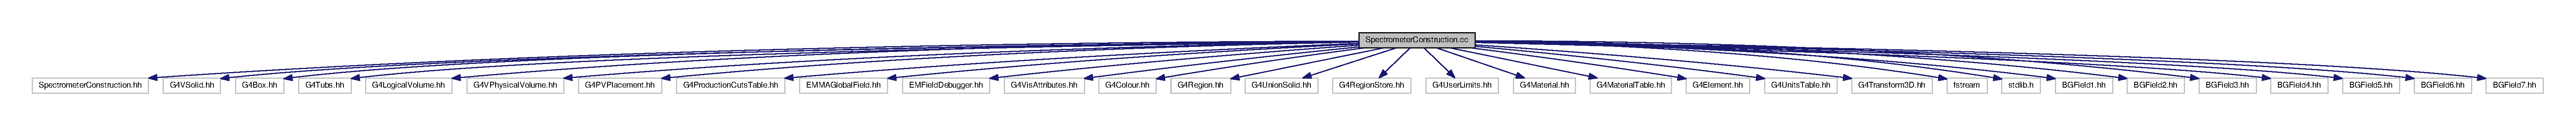
\includegraphics[width=350pt]{SpectrometerConstruction_8cc__incl}
\end{center}
\end{figure}
\subsection*{Variables}
\begin{DoxyCompactItemize}
\item 
G4double \hyperlink{SpectrometerConstruction_8cc_a63b4d37f848ab857400025988ebc68ac}{z\+Q1begins}
\item 
G4double \hyperlink{SpectrometerConstruction_8cc_aaefdf69418ceee3aabc72a346eef1799}{z\+Q4ends}
\item 
G4double \hyperlink{SpectrometerConstruction_8cc_a9906ccfd8985bb28a72c37e7cd16f277}{z\+Anode}
\item 
G4double \hyperlink{SpectrometerConstruction_8cc_a499096b9dc56ffa559bd1aec0bafe28e}{z\+Focal\+Plane}
\item 
G4double \hyperlink{SpectrometerConstruction_8cc_a8825e4bac9c627d0fc56ceb808baee99}{z\+Q1ends}
\item 
G4double \hyperlink{SpectrometerConstruction_8cc_a0389aed4a205ff7970a9c57db9776625}{z\+Q2ends}
\item 
G4double \hyperlink{SpectrometerConstruction_8cc_aa309293d04a3e9edd55505001bb8842f}{z\+Q3ends}
\item 
G4double \hyperlink{SpectrometerConstruction_8cc_a62d0de84d7d6b0923e982b354afad285}{z\+Q2begins}
\item 
G4double \hyperlink{SpectrometerConstruction_8cc_a12daa717eecd47b0ce06c1314040fc3c}{z\+Q3begins}
\item 
G4double \hyperlink{SpectrometerConstruction_8cc_ab2b8c71527a18e35d81eb8bd6e7691f4}{z\+Q4begins}
\item 
G4double \hyperlink{SpectrometerConstruction_8cc_aad92ec801d3e4699e64b73238d977d97}{z\+Q1fieldbegins}
\item 
G4double \hyperlink{SpectrometerConstruction_8cc_a312fb44f7507d957ccc70c34d5d94a43}{z\+Q2fieldbegins}
\item 
G4double \hyperlink{SpectrometerConstruction_8cc_a92fc8c51d58e20801f34d52f8a2c7a2b}{z\+Q2fieldends}
\item 
G4double \hyperlink{SpectrometerConstruction_8cc_a077f13a115281633166d7450d5f26fa0}{z\+Q3fieldbegins}
\item 
G4double \hyperlink{SpectrometerConstruction_8cc_afb3a8a6427088f204ef91b7361831904}{z\+Q4fieldbegins}
\item 
G4double \hyperlink{SpectrometerConstruction_8cc_a2f06aa9a2a32a33fa1100ce176ab4636}{z\+Q4fieldends}
\item 
G4double \hyperlink{SpectrometerConstruction_8cc_a3feee11b7c51f66f2b05335422fd6766}{z\+E\+D1fieldbegins}
\item 
G4double \hyperlink{SpectrometerConstruction_8cc_ab9ae78ef340f126ece97727282006616}{x\+E\+D1fieldends}
\item 
G4double \hyperlink{SpectrometerConstruction_8cc_a233a000653cf27b6f9124c2a55731df1}{z\+E\+D1fieldends}
\item 
G4double \hyperlink{SpectrometerConstruction_8cc_a20f1012cd491461a26923d2c5e7bf9e9}{x\+M\+Dfieldbegins}
\item 
G4double \hyperlink{SpectrometerConstruction_8cc_a69783c655a650a2d465aa29adb99becd}{z\+M\+Dfieldbegins}
\item 
G4double \hyperlink{SpectrometerConstruction_8cc_a159fc7800979fa9630bfc45a7f78596c}{x\+M\+Dfieldends}
\item 
G4double \hyperlink{SpectrometerConstruction_8cc_ac69dbd129f1b938df9976d51f7593e8d}{z\+M\+Dfieldends}
\item 
G4double \hyperlink{SpectrometerConstruction_8cc_a1756cc9671bdb5e3fef3244359b6d3cc}{x\+E\+D2fieldbegins}
\item 
G4double \hyperlink{SpectrometerConstruction_8cc_ad016826f85af9d76258e59348edeb364}{z\+E\+D2fieldbegins}
\item 
G4double \hyperlink{SpectrometerConstruction_8cc_a9d0bd55552fe4d1f2f44f49d35cc081e}{z\+E\+D2fieldends}
\item 
G4double \hyperlink{SpectrometerConstruction_8cc_a244d4cfe9b2fed8a950b5260924858ff}{x\+E\+D1center}
\item 
G4double \hyperlink{SpectrometerConstruction_8cc_a74ebfc53f3a93114f6d28295ee4ab9f4}{z\+E\+D1center}
\item 
G4double \hyperlink{SpectrometerConstruction_8cc_a3c58a920166faad49e1879314c55c5be}{x\+E\+D2center}
\item 
G4double \hyperlink{SpectrometerConstruction_8cc_ac98e44690840a121652fcb08b156a635}{z\+E\+D2center}
\item 
G4double \hyperlink{SpectrometerConstruction_8cc_a715d053d73470185e7c2c4702d9dc2de}{r\+ED}
\item 
G4double \hyperlink{SpectrometerConstruction_8cc_aebdd7edbdb400c898923e8d3722725bf}{x\+M\+Dcenter}
\item 
G4double \hyperlink{SpectrometerConstruction_8cc_ac5e70ecd77b70fb29053de3d744defbe}{z\+M\+Dcenter}
\item 
G4double \hyperlink{SpectrometerConstruction_8cc_a7fd4fbedfa36308277282111f3a02a2e}{r\+MD}
\item 
G4double \hyperlink{SpectrometerConstruction_8cc_a6a82266fb838ffa86812c6000c9dc287}{Q1before}
\item 
G4double \hyperlink{SpectrometerConstruction_8cc_a5566ea3bf099349decdfcf3c26fc376c}{Q2before}
\item 
G4double \hyperlink{SpectrometerConstruction_8cc_a75fe85cecce8dd0b8fa08cf97cee4ce2}{E\+D1before}
\item 
G4double \hyperlink{SpectrometerConstruction_8cc_a003204f9438882eab89ba42ae5708f37}{M\+Dbefore}
\item 
G4double \hyperlink{SpectrometerConstruction_8cc_a1fb2ee29034baaf6ed6e2acbdbf8b578}{E\+D2before}
\item 
G4double \hyperlink{SpectrometerConstruction_8cc_a2fe0c19691575193f51b8ef4c4301aad}{Q3before}
\item 
G4double \hyperlink{SpectrometerConstruction_8cc_a807b9ab7f57ec0c8bdc7764053d3e516}{Q4before}
\item 
G4double \hyperlink{SpectrometerConstruction_8cc_a79e8de762c55f46eaf341c33ddcdfabd}{Q1after}
\item 
G4double \hyperlink{SpectrometerConstruction_8cc_a9d33b4b693d4f7341602ab26cb44359c}{Q2after}
\item 
G4double \hyperlink{SpectrometerConstruction_8cc_a56c3dd0f81ddd6f90cfcc044fb51dff1}{E\+D1after}
\item 
G4double \hyperlink{SpectrometerConstruction_8cc_af04f7784a3cdd89375e6c74b915d255c}{M\+Dafter}
\item 
G4double \hyperlink{SpectrometerConstruction_8cc_ad4c429af59f2e7eee31d1480df299599}{E\+D2after}
\item 
G4double \hyperlink{SpectrometerConstruction_8cc_a7a55e4b1397f5859cde14aa271bb3717}{Q3after}
\item 
G4double \hyperlink{SpectrometerConstruction_8cc_a47d7897cbc13a67cc420cfb3ec97fd60}{Q4after}
\item 
G4double \hyperlink{SpectrometerConstruction_8cc_a58acf77da23d6d58252d729d4d8212d1}{Pipe4z}
\item 
G4double \hyperlink{SpectrometerConstruction_8cc_ab20b3e8fa2797e410fb9110cfad39796}{Pipe4\+HL}
\item 
G4double \hyperlink{SpectrometerConstruction_8cc_a7369eeb2c228d92eeb2a6e7ad496e13f}{Pipe7\+HL}
\item 
G4\+String \hyperlink{SpectrometerConstruction_8cc_ae9b14cfeccc31b1bf76af2f4c3aae43d}{field\+File\+Name}
\item 
G4\+String \hyperlink{SpectrometerConstruction_8cc_a8558631b93942e4ae79b3feb21c97c8f}{User\+Dir}
\end{DoxyCompactItemize}


\subsection{Variable Documentation}
\index{Spectrometer\+Construction.\+cc@{Spectrometer\+Construction.\+cc}!E\+D1after@{E\+D1after}}
\index{E\+D1after@{E\+D1after}!Spectrometer\+Construction.\+cc@{Spectrometer\+Construction.\+cc}}
\subsubsection[{\texorpdfstring{E\+D1after}{ED1after}}]{\setlength{\rightskip}{0pt plus 5cm}G4double E\+D1after}\hypertarget{SpectrometerConstruction_8cc_a56c3dd0f81ddd6f90cfcc044fb51dff1}{}\label{SpectrometerConstruction_8cc_a56c3dd0f81ddd6f90cfcc044fb51dff1}
\index{Spectrometer\+Construction.\+cc@{Spectrometer\+Construction.\+cc}!E\+D1before@{E\+D1before}}
\index{E\+D1before@{E\+D1before}!Spectrometer\+Construction.\+cc@{Spectrometer\+Construction.\+cc}}
\subsubsection[{\texorpdfstring{E\+D1before}{ED1before}}]{\setlength{\rightskip}{0pt plus 5cm}G4double E\+D1before}\hypertarget{SpectrometerConstruction_8cc_a75fe85cecce8dd0b8fa08cf97cee4ce2}{}\label{SpectrometerConstruction_8cc_a75fe85cecce8dd0b8fa08cf97cee4ce2}
\index{Spectrometer\+Construction.\+cc@{Spectrometer\+Construction.\+cc}!E\+D2after@{E\+D2after}}
\index{E\+D2after@{E\+D2after}!Spectrometer\+Construction.\+cc@{Spectrometer\+Construction.\+cc}}
\subsubsection[{\texorpdfstring{E\+D2after}{ED2after}}]{\setlength{\rightskip}{0pt plus 5cm}G4double E\+D2after}\hypertarget{SpectrometerConstruction_8cc_ad4c429af59f2e7eee31d1480df299599}{}\label{SpectrometerConstruction_8cc_ad4c429af59f2e7eee31d1480df299599}
\index{Spectrometer\+Construction.\+cc@{Spectrometer\+Construction.\+cc}!E\+D2before@{E\+D2before}}
\index{E\+D2before@{E\+D2before}!Spectrometer\+Construction.\+cc@{Spectrometer\+Construction.\+cc}}
\subsubsection[{\texorpdfstring{E\+D2before}{ED2before}}]{\setlength{\rightskip}{0pt plus 5cm}G4double E\+D2before}\hypertarget{SpectrometerConstruction_8cc_a1fb2ee29034baaf6ed6e2acbdbf8b578}{}\label{SpectrometerConstruction_8cc_a1fb2ee29034baaf6ed6e2acbdbf8b578}
\index{Spectrometer\+Construction.\+cc@{Spectrometer\+Construction.\+cc}!field\+File\+Name@{field\+File\+Name}}
\index{field\+File\+Name@{field\+File\+Name}!Spectrometer\+Construction.\+cc@{Spectrometer\+Construction.\+cc}}
\subsubsection[{\texorpdfstring{field\+File\+Name}{fieldFileName}}]{\setlength{\rightskip}{0pt plus 5cm}G4\+String field\+File\+Name}\hypertarget{SpectrometerConstruction_8cc_ae9b14cfeccc31b1bf76af2f4c3aae43d}{}\label{SpectrometerConstruction_8cc_ae9b14cfeccc31b1bf76af2f4c3aae43d}
\index{Spectrometer\+Construction.\+cc@{Spectrometer\+Construction.\+cc}!M\+Dafter@{M\+Dafter}}
\index{M\+Dafter@{M\+Dafter}!Spectrometer\+Construction.\+cc@{Spectrometer\+Construction.\+cc}}
\subsubsection[{\texorpdfstring{M\+Dafter}{MDafter}}]{\setlength{\rightskip}{0pt plus 5cm}G4double M\+Dafter}\hypertarget{SpectrometerConstruction_8cc_af04f7784a3cdd89375e6c74b915d255c}{}\label{SpectrometerConstruction_8cc_af04f7784a3cdd89375e6c74b915d255c}
\index{Spectrometer\+Construction.\+cc@{Spectrometer\+Construction.\+cc}!M\+Dbefore@{M\+Dbefore}}
\index{M\+Dbefore@{M\+Dbefore}!Spectrometer\+Construction.\+cc@{Spectrometer\+Construction.\+cc}}
\subsubsection[{\texorpdfstring{M\+Dbefore}{MDbefore}}]{\setlength{\rightskip}{0pt plus 5cm}G4double M\+Dbefore}\hypertarget{SpectrometerConstruction_8cc_a003204f9438882eab89ba42ae5708f37}{}\label{SpectrometerConstruction_8cc_a003204f9438882eab89ba42ae5708f37}
\index{Spectrometer\+Construction.\+cc@{Spectrometer\+Construction.\+cc}!Pipe4\+HL@{Pipe4\+HL}}
\index{Pipe4\+HL@{Pipe4\+HL}!Spectrometer\+Construction.\+cc@{Spectrometer\+Construction.\+cc}}
\subsubsection[{\texorpdfstring{Pipe4\+HL}{Pipe4HL}}]{\setlength{\rightskip}{0pt plus 5cm}G4double Pipe4\+HL}\hypertarget{SpectrometerConstruction_8cc_ab20b3e8fa2797e410fb9110cfad39796}{}\label{SpectrometerConstruction_8cc_ab20b3e8fa2797e410fb9110cfad39796}
\index{Spectrometer\+Construction.\+cc@{Spectrometer\+Construction.\+cc}!Pipe4z@{Pipe4z}}
\index{Pipe4z@{Pipe4z}!Spectrometer\+Construction.\+cc@{Spectrometer\+Construction.\+cc}}
\subsubsection[{\texorpdfstring{Pipe4z}{Pipe4z}}]{\setlength{\rightskip}{0pt plus 5cm}G4double Pipe4z}\hypertarget{SpectrometerConstruction_8cc_a58acf77da23d6d58252d729d4d8212d1}{}\label{SpectrometerConstruction_8cc_a58acf77da23d6d58252d729d4d8212d1}
\index{Spectrometer\+Construction.\+cc@{Spectrometer\+Construction.\+cc}!Pipe7\+HL@{Pipe7\+HL}}
\index{Pipe7\+HL@{Pipe7\+HL}!Spectrometer\+Construction.\+cc@{Spectrometer\+Construction.\+cc}}
\subsubsection[{\texorpdfstring{Pipe7\+HL}{Pipe7HL}}]{\setlength{\rightskip}{0pt plus 5cm}G4double Pipe7\+HL}\hypertarget{SpectrometerConstruction_8cc_a7369eeb2c228d92eeb2a6e7ad496e13f}{}\label{SpectrometerConstruction_8cc_a7369eeb2c228d92eeb2a6e7ad496e13f}
\index{Spectrometer\+Construction.\+cc@{Spectrometer\+Construction.\+cc}!Q1after@{Q1after}}
\index{Q1after@{Q1after}!Spectrometer\+Construction.\+cc@{Spectrometer\+Construction.\+cc}}
\subsubsection[{\texorpdfstring{Q1after}{Q1after}}]{\setlength{\rightskip}{0pt plus 5cm}G4double Q1after}\hypertarget{SpectrometerConstruction_8cc_a79e8de762c55f46eaf341c33ddcdfabd}{}\label{SpectrometerConstruction_8cc_a79e8de762c55f46eaf341c33ddcdfabd}
\index{Spectrometer\+Construction.\+cc@{Spectrometer\+Construction.\+cc}!Q1before@{Q1before}}
\index{Q1before@{Q1before}!Spectrometer\+Construction.\+cc@{Spectrometer\+Construction.\+cc}}
\subsubsection[{\texorpdfstring{Q1before}{Q1before}}]{\setlength{\rightskip}{0pt plus 5cm}G4double Q1before}\hypertarget{SpectrometerConstruction_8cc_a6a82266fb838ffa86812c6000c9dc287}{}\label{SpectrometerConstruction_8cc_a6a82266fb838ffa86812c6000c9dc287}
\index{Spectrometer\+Construction.\+cc@{Spectrometer\+Construction.\+cc}!Q2after@{Q2after}}
\index{Q2after@{Q2after}!Spectrometer\+Construction.\+cc@{Spectrometer\+Construction.\+cc}}
\subsubsection[{\texorpdfstring{Q2after}{Q2after}}]{\setlength{\rightskip}{0pt plus 5cm}G4double Q2after}\hypertarget{SpectrometerConstruction_8cc_a9d33b4b693d4f7341602ab26cb44359c}{}\label{SpectrometerConstruction_8cc_a9d33b4b693d4f7341602ab26cb44359c}
\index{Spectrometer\+Construction.\+cc@{Spectrometer\+Construction.\+cc}!Q2before@{Q2before}}
\index{Q2before@{Q2before}!Spectrometer\+Construction.\+cc@{Spectrometer\+Construction.\+cc}}
\subsubsection[{\texorpdfstring{Q2before}{Q2before}}]{\setlength{\rightskip}{0pt plus 5cm}G4double Q2before}\hypertarget{SpectrometerConstruction_8cc_a5566ea3bf099349decdfcf3c26fc376c}{}\label{SpectrometerConstruction_8cc_a5566ea3bf099349decdfcf3c26fc376c}
\index{Spectrometer\+Construction.\+cc@{Spectrometer\+Construction.\+cc}!Q3after@{Q3after}}
\index{Q3after@{Q3after}!Spectrometer\+Construction.\+cc@{Spectrometer\+Construction.\+cc}}
\subsubsection[{\texorpdfstring{Q3after}{Q3after}}]{\setlength{\rightskip}{0pt plus 5cm}G4double Q3after}\hypertarget{SpectrometerConstruction_8cc_a7a55e4b1397f5859cde14aa271bb3717}{}\label{SpectrometerConstruction_8cc_a7a55e4b1397f5859cde14aa271bb3717}
\index{Spectrometer\+Construction.\+cc@{Spectrometer\+Construction.\+cc}!Q3before@{Q3before}}
\index{Q3before@{Q3before}!Spectrometer\+Construction.\+cc@{Spectrometer\+Construction.\+cc}}
\subsubsection[{\texorpdfstring{Q3before}{Q3before}}]{\setlength{\rightskip}{0pt plus 5cm}G4double Q3before}\hypertarget{SpectrometerConstruction_8cc_a2fe0c19691575193f51b8ef4c4301aad}{}\label{SpectrometerConstruction_8cc_a2fe0c19691575193f51b8ef4c4301aad}
\index{Spectrometer\+Construction.\+cc@{Spectrometer\+Construction.\+cc}!Q4after@{Q4after}}
\index{Q4after@{Q4after}!Spectrometer\+Construction.\+cc@{Spectrometer\+Construction.\+cc}}
\subsubsection[{\texorpdfstring{Q4after}{Q4after}}]{\setlength{\rightskip}{0pt plus 5cm}G4double Q4after}\hypertarget{SpectrometerConstruction_8cc_a47d7897cbc13a67cc420cfb3ec97fd60}{}\label{SpectrometerConstruction_8cc_a47d7897cbc13a67cc420cfb3ec97fd60}
\index{Spectrometer\+Construction.\+cc@{Spectrometer\+Construction.\+cc}!Q4before@{Q4before}}
\index{Q4before@{Q4before}!Spectrometer\+Construction.\+cc@{Spectrometer\+Construction.\+cc}}
\subsubsection[{\texorpdfstring{Q4before}{Q4before}}]{\setlength{\rightskip}{0pt plus 5cm}G4double Q4before}\hypertarget{SpectrometerConstruction_8cc_a807b9ab7f57ec0c8bdc7764053d3e516}{}\label{SpectrometerConstruction_8cc_a807b9ab7f57ec0c8bdc7764053d3e516}
\index{Spectrometer\+Construction.\+cc@{Spectrometer\+Construction.\+cc}!r\+ED@{r\+ED}}
\index{r\+ED@{r\+ED}!Spectrometer\+Construction.\+cc@{Spectrometer\+Construction.\+cc}}
\subsubsection[{\texorpdfstring{r\+ED}{rED}}]{\setlength{\rightskip}{0pt plus 5cm}G4double r\+ED}\hypertarget{SpectrometerConstruction_8cc_a715d053d73470185e7c2c4702d9dc2de}{}\label{SpectrometerConstruction_8cc_a715d053d73470185e7c2c4702d9dc2de}
\index{Spectrometer\+Construction.\+cc@{Spectrometer\+Construction.\+cc}!r\+MD@{r\+MD}}
\index{r\+MD@{r\+MD}!Spectrometer\+Construction.\+cc@{Spectrometer\+Construction.\+cc}}
\subsubsection[{\texorpdfstring{r\+MD}{rMD}}]{\setlength{\rightskip}{0pt plus 5cm}G4double r\+MD}\hypertarget{SpectrometerConstruction_8cc_a7fd4fbedfa36308277282111f3a02a2e}{}\label{SpectrometerConstruction_8cc_a7fd4fbedfa36308277282111f3a02a2e}
\index{Spectrometer\+Construction.\+cc@{Spectrometer\+Construction.\+cc}!User\+Dir@{User\+Dir}}
\index{User\+Dir@{User\+Dir}!Spectrometer\+Construction.\+cc@{Spectrometer\+Construction.\+cc}}
\subsubsection[{\texorpdfstring{User\+Dir}{UserDir}}]{\setlength{\rightskip}{0pt plus 5cm}G4\+String User\+Dir}\hypertarget{SpectrometerConstruction_8cc_a8558631b93942e4ae79b3feb21c97c8f}{}\label{SpectrometerConstruction_8cc_a8558631b93942e4ae79b3feb21c97c8f}
\index{Spectrometer\+Construction.\+cc@{Spectrometer\+Construction.\+cc}!x\+E\+D1center@{x\+E\+D1center}}
\index{x\+E\+D1center@{x\+E\+D1center}!Spectrometer\+Construction.\+cc@{Spectrometer\+Construction.\+cc}}
\subsubsection[{\texorpdfstring{x\+E\+D1center}{xED1center}}]{\setlength{\rightskip}{0pt plus 5cm}G4double x\+E\+D1center}\hypertarget{SpectrometerConstruction_8cc_a244d4cfe9b2fed8a950b5260924858ff}{}\label{SpectrometerConstruction_8cc_a244d4cfe9b2fed8a950b5260924858ff}
\index{Spectrometer\+Construction.\+cc@{Spectrometer\+Construction.\+cc}!x\+E\+D1fieldends@{x\+E\+D1fieldends}}
\index{x\+E\+D1fieldends@{x\+E\+D1fieldends}!Spectrometer\+Construction.\+cc@{Spectrometer\+Construction.\+cc}}
\subsubsection[{\texorpdfstring{x\+E\+D1fieldends}{xED1fieldends}}]{\setlength{\rightskip}{0pt plus 5cm}G4double x\+E\+D1fieldends}\hypertarget{SpectrometerConstruction_8cc_ab9ae78ef340f126ece97727282006616}{}\label{SpectrometerConstruction_8cc_ab9ae78ef340f126ece97727282006616}
\index{Spectrometer\+Construction.\+cc@{Spectrometer\+Construction.\+cc}!x\+E\+D2center@{x\+E\+D2center}}
\index{x\+E\+D2center@{x\+E\+D2center}!Spectrometer\+Construction.\+cc@{Spectrometer\+Construction.\+cc}}
\subsubsection[{\texorpdfstring{x\+E\+D2center}{xED2center}}]{\setlength{\rightskip}{0pt plus 5cm}G4double x\+E\+D2center}\hypertarget{SpectrometerConstruction_8cc_a3c58a920166faad49e1879314c55c5be}{}\label{SpectrometerConstruction_8cc_a3c58a920166faad49e1879314c55c5be}
\index{Spectrometer\+Construction.\+cc@{Spectrometer\+Construction.\+cc}!x\+E\+D2fieldbegins@{x\+E\+D2fieldbegins}}
\index{x\+E\+D2fieldbegins@{x\+E\+D2fieldbegins}!Spectrometer\+Construction.\+cc@{Spectrometer\+Construction.\+cc}}
\subsubsection[{\texorpdfstring{x\+E\+D2fieldbegins}{xED2fieldbegins}}]{\setlength{\rightskip}{0pt plus 5cm}G4double x\+E\+D2fieldbegins}\hypertarget{SpectrometerConstruction_8cc_a1756cc9671bdb5e3fef3244359b6d3cc}{}\label{SpectrometerConstruction_8cc_a1756cc9671bdb5e3fef3244359b6d3cc}
\index{Spectrometer\+Construction.\+cc@{Spectrometer\+Construction.\+cc}!x\+M\+Dcenter@{x\+M\+Dcenter}}
\index{x\+M\+Dcenter@{x\+M\+Dcenter}!Spectrometer\+Construction.\+cc@{Spectrometer\+Construction.\+cc}}
\subsubsection[{\texorpdfstring{x\+M\+Dcenter}{xMDcenter}}]{\setlength{\rightskip}{0pt plus 5cm}G4double x\+M\+Dcenter}\hypertarget{SpectrometerConstruction_8cc_aebdd7edbdb400c898923e8d3722725bf}{}\label{SpectrometerConstruction_8cc_aebdd7edbdb400c898923e8d3722725bf}
\index{Spectrometer\+Construction.\+cc@{Spectrometer\+Construction.\+cc}!x\+M\+Dfieldbegins@{x\+M\+Dfieldbegins}}
\index{x\+M\+Dfieldbegins@{x\+M\+Dfieldbegins}!Spectrometer\+Construction.\+cc@{Spectrometer\+Construction.\+cc}}
\subsubsection[{\texorpdfstring{x\+M\+Dfieldbegins}{xMDfieldbegins}}]{\setlength{\rightskip}{0pt plus 5cm}G4double x\+M\+Dfieldbegins}\hypertarget{SpectrometerConstruction_8cc_a20f1012cd491461a26923d2c5e7bf9e9}{}\label{SpectrometerConstruction_8cc_a20f1012cd491461a26923d2c5e7bf9e9}
\index{Spectrometer\+Construction.\+cc@{Spectrometer\+Construction.\+cc}!x\+M\+Dfieldends@{x\+M\+Dfieldends}}
\index{x\+M\+Dfieldends@{x\+M\+Dfieldends}!Spectrometer\+Construction.\+cc@{Spectrometer\+Construction.\+cc}}
\subsubsection[{\texorpdfstring{x\+M\+Dfieldends}{xMDfieldends}}]{\setlength{\rightskip}{0pt plus 5cm}G4double x\+M\+Dfieldends}\hypertarget{SpectrometerConstruction_8cc_a159fc7800979fa9630bfc45a7f78596c}{}\label{SpectrometerConstruction_8cc_a159fc7800979fa9630bfc45a7f78596c}
\index{Spectrometer\+Construction.\+cc@{Spectrometer\+Construction.\+cc}!z\+Anode@{z\+Anode}}
\index{z\+Anode@{z\+Anode}!Spectrometer\+Construction.\+cc@{Spectrometer\+Construction.\+cc}}
\subsubsection[{\texorpdfstring{z\+Anode}{zAnode}}]{\setlength{\rightskip}{0pt plus 5cm}G4double z\+Anode}\hypertarget{SpectrometerConstruction_8cc_a9906ccfd8985bb28a72c37e7cd16f277}{}\label{SpectrometerConstruction_8cc_a9906ccfd8985bb28a72c37e7cd16f277}
\index{Spectrometer\+Construction.\+cc@{Spectrometer\+Construction.\+cc}!z\+E\+D1center@{z\+E\+D1center}}
\index{z\+E\+D1center@{z\+E\+D1center}!Spectrometer\+Construction.\+cc@{Spectrometer\+Construction.\+cc}}
\subsubsection[{\texorpdfstring{z\+E\+D1center}{zED1center}}]{\setlength{\rightskip}{0pt plus 5cm}G4double z\+E\+D1center}\hypertarget{SpectrometerConstruction_8cc_a74ebfc53f3a93114f6d28295ee4ab9f4}{}\label{SpectrometerConstruction_8cc_a74ebfc53f3a93114f6d28295ee4ab9f4}
\index{Spectrometer\+Construction.\+cc@{Spectrometer\+Construction.\+cc}!z\+E\+D1fieldbegins@{z\+E\+D1fieldbegins}}
\index{z\+E\+D1fieldbegins@{z\+E\+D1fieldbegins}!Spectrometer\+Construction.\+cc@{Spectrometer\+Construction.\+cc}}
\subsubsection[{\texorpdfstring{z\+E\+D1fieldbegins}{zED1fieldbegins}}]{\setlength{\rightskip}{0pt plus 5cm}G4double z\+E\+D1fieldbegins}\hypertarget{SpectrometerConstruction_8cc_a3feee11b7c51f66f2b05335422fd6766}{}\label{SpectrometerConstruction_8cc_a3feee11b7c51f66f2b05335422fd6766}
\index{Spectrometer\+Construction.\+cc@{Spectrometer\+Construction.\+cc}!z\+E\+D1fieldends@{z\+E\+D1fieldends}}
\index{z\+E\+D1fieldends@{z\+E\+D1fieldends}!Spectrometer\+Construction.\+cc@{Spectrometer\+Construction.\+cc}}
\subsubsection[{\texorpdfstring{z\+E\+D1fieldends}{zED1fieldends}}]{\setlength{\rightskip}{0pt plus 5cm}G4double z\+E\+D1fieldends}\hypertarget{SpectrometerConstruction_8cc_a233a000653cf27b6f9124c2a55731df1}{}\label{SpectrometerConstruction_8cc_a233a000653cf27b6f9124c2a55731df1}
\index{Spectrometer\+Construction.\+cc@{Spectrometer\+Construction.\+cc}!z\+E\+D2center@{z\+E\+D2center}}
\index{z\+E\+D2center@{z\+E\+D2center}!Spectrometer\+Construction.\+cc@{Spectrometer\+Construction.\+cc}}
\subsubsection[{\texorpdfstring{z\+E\+D2center}{zED2center}}]{\setlength{\rightskip}{0pt plus 5cm}G4double z\+E\+D2center}\hypertarget{SpectrometerConstruction_8cc_ac98e44690840a121652fcb08b156a635}{}\label{SpectrometerConstruction_8cc_ac98e44690840a121652fcb08b156a635}
\index{Spectrometer\+Construction.\+cc@{Spectrometer\+Construction.\+cc}!z\+E\+D2fieldbegins@{z\+E\+D2fieldbegins}}
\index{z\+E\+D2fieldbegins@{z\+E\+D2fieldbegins}!Spectrometer\+Construction.\+cc@{Spectrometer\+Construction.\+cc}}
\subsubsection[{\texorpdfstring{z\+E\+D2fieldbegins}{zED2fieldbegins}}]{\setlength{\rightskip}{0pt plus 5cm}G4double z\+E\+D2fieldbegins}\hypertarget{SpectrometerConstruction_8cc_ad016826f85af9d76258e59348edeb364}{}\label{SpectrometerConstruction_8cc_ad016826f85af9d76258e59348edeb364}
\index{Spectrometer\+Construction.\+cc@{Spectrometer\+Construction.\+cc}!z\+E\+D2fieldends@{z\+E\+D2fieldends}}
\index{z\+E\+D2fieldends@{z\+E\+D2fieldends}!Spectrometer\+Construction.\+cc@{Spectrometer\+Construction.\+cc}}
\subsubsection[{\texorpdfstring{z\+E\+D2fieldends}{zED2fieldends}}]{\setlength{\rightskip}{0pt plus 5cm}G4double z\+E\+D2fieldends}\hypertarget{SpectrometerConstruction_8cc_a9d0bd55552fe4d1f2f44f49d35cc081e}{}\label{SpectrometerConstruction_8cc_a9d0bd55552fe4d1f2f44f49d35cc081e}
\index{Spectrometer\+Construction.\+cc@{Spectrometer\+Construction.\+cc}!z\+Focal\+Plane@{z\+Focal\+Plane}}
\index{z\+Focal\+Plane@{z\+Focal\+Plane}!Spectrometer\+Construction.\+cc@{Spectrometer\+Construction.\+cc}}
\subsubsection[{\texorpdfstring{z\+Focal\+Plane}{zFocalPlane}}]{\setlength{\rightskip}{0pt plus 5cm}G4double z\+Focal\+Plane}\hypertarget{SpectrometerConstruction_8cc_a499096b9dc56ffa559bd1aec0bafe28e}{}\label{SpectrometerConstruction_8cc_a499096b9dc56ffa559bd1aec0bafe28e}
\index{Spectrometer\+Construction.\+cc@{Spectrometer\+Construction.\+cc}!z\+M\+Dcenter@{z\+M\+Dcenter}}
\index{z\+M\+Dcenter@{z\+M\+Dcenter}!Spectrometer\+Construction.\+cc@{Spectrometer\+Construction.\+cc}}
\subsubsection[{\texorpdfstring{z\+M\+Dcenter}{zMDcenter}}]{\setlength{\rightskip}{0pt plus 5cm}G4double z\+M\+Dcenter}\hypertarget{SpectrometerConstruction_8cc_ac5e70ecd77b70fb29053de3d744defbe}{}\label{SpectrometerConstruction_8cc_ac5e70ecd77b70fb29053de3d744defbe}
\index{Spectrometer\+Construction.\+cc@{Spectrometer\+Construction.\+cc}!z\+M\+Dfieldbegins@{z\+M\+Dfieldbegins}}
\index{z\+M\+Dfieldbegins@{z\+M\+Dfieldbegins}!Spectrometer\+Construction.\+cc@{Spectrometer\+Construction.\+cc}}
\subsubsection[{\texorpdfstring{z\+M\+Dfieldbegins}{zMDfieldbegins}}]{\setlength{\rightskip}{0pt plus 5cm}G4double z\+M\+Dfieldbegins}\hypertarget{SpectrometerConstruction_8cc_a69783c655a650a2d465aa29adb99becd}{}\label{SpectrometerConstruction_8cc_a69783c655a650a2d465aa29adb99becd}
\index{Spectrometer\+Construction.\+cc@{Spectrometer\+Construction.\+cc}!z\+M\+Dfieldends@{z\+M\+Dfieldends}}
\index{z\+M\+Dfieldends@{z\+M\+Dfieldends}!Spectrometer\+Construction.\+cc@{Spectrometer\+Construction.\+cc}}
\subsubsection[{\texorpdfstring{z\+M\+Dfieldends}{zMDfieldends}}]{\setlength{\rightskip}{0pt plus 5cm}G4double z\+M\+Dfieldends}\hypertarget{SpectrometerConstruction_8cc_ac69dbd129f1b938df9976d51f7593e8d}{}\label{SpectrometerConstruction_8cc_ac69dbd129f1b938df9976d51f7593e8d}
\index{Spectrometer\+Construction.\+cc@{Spectrometer\+Construction.\+cc}!z\+Q1begins@{z\+Q1begins}}
\index{z\+Q1begins@{z\+Q1begins}!Spectrometer\+Construction.\+cc@{Spectrometer\+Construction.\+cc}}
\subsubsection[{\texorpdfstring{z\+Q1begins}{zQ1begins}}]{\setlength{\rightskip}{0pt plus 5cm}G4double z\+Q1begins}\hypertarget{SpectrometerConstruction_8cc_a63b4d37f848ab857400025988ebc68ac}{}\label{SpectrometerConstruction_8cc_a63b4d37f848ab857400025988ebc68ac}
\index{Spectrometer\+Construction.\+cc@{Spectrometer\+Construction.\+cc}!z\+Q1ends@{z\+Q1ends}}
\index{z\+Q1ends@{z\+Q1ends}!Spectrometer\+Construction.\+cc@{Spectrometer\+Construction.\+cc}}
\subsubsection[{\texorpdfstring{z\+Q1ends}{zQ1ends}}]{\setlength{\rightskip}{0pt plus 5cm}G4double z\+Q1ends}\hypertarget{SpectrometerConstruction_8cc_a8825e4bac9c627d0fc56ceb808baee99}{}\label{SpectrometerConstruction_8cc_a8825e4bac9c627d0fc56ceb808baee99}
\index{Spectrometer\+Construction.\+cc@{Spectrometer\+Construction.\+cc}!z\+Q1fieldbegins@{z\+Q1fieldbegins}}
\index{z\+Q1fieldbegins@{z\+Q1fieldbegins}!Spectrometer\+Construction.\+cc@{Spectrometer\+Construction.\+cc}}
\subsubsection[{\texorpdfstring{z\+Q1fieldbegins}{zQ1fieldbegins}}]{\setlength{\rightskip}{0pt plus 5cm}G4double z\+Q1fieldbegins}\hypertarget{SpectrometerConstruction_8cc_aad92ec801d3e4699e64b73238d977d97}{}\label{SpectrometerConstruction_8cc_aad92ec801d3e4699e64b73238d977d97}
\index{Spectrometer\+Construction.\+cc@{Spectrometer\+Construction.\+cc}!z\+Q2begins@{z\+Q2begins}}
\index{z\+Q2begins@{z\+Q2begins}!Spectrometer\+Construction.\+cc@{Spectrometer\+Construction.\+cc}}
\subsubsection[{\texorpdfstring{z\+Q2begins}{zQ2begins}}]{\setlength{\rightskip}{0pt plus 5cm}G4double z\+Q2begins}\hypertarget{SpectrometerConstruction_8cc_a62d0de84d7d6b0923e982b354afad285}{}\label{SpectrometerConstruction_8cc_a62d0de84d7d6b0923e982b354afad285}
\index{Spectrometer\+Construction.\+cc@{Spectrometer\+Construction.\+cc}!z\+Q2ends@{z\+Q2ends}}
\index{z\+Q2ends@{z\+Q2ends}!Spectrometer\+Construction.\+cc@{Spectrometer\+Construction.\+cc}}
\subsubsection[{\texorpdfstring{z\+Q2ends}{zQ2ends}}]{\setlength{\rightskip}{0pt plus 5cm}G4double z\+Q2ends}\hypertarget{SpectrometerConstruction_8cc_a0389aed4a205ff7970a9c57db9776625}{}\label{SpectrometerConstruction_8cc_a0389aed4a205ff7970a9c57db9776625}
\index{Spectrometer\+Construction.\+cc@{Spectrometer\+Construction.\+cc}!z\+Q2fieldbegins@{z\+Q2fieldbegins}}
\index{z\+Q2fieldbegins@{z\+Q2fieldbegins}!Spectrometer\+Construction.\+cc@{Spectrometer\+Construction.\+cc}}
\subsubsection[{\texorpdfstring{z\+Q2fieldbegins}{zQ2fieldbegins}}]{\setlength{\rightskip}{0pt plus 5cm}G4double z\+Q2fieldbegins}\hypertarget{SpectrometerConstruction_8cc_a312fb44f7507d957ccc70c34d5d94a43}{}\label{SpectrometerConstruction_8cc_a312fb44f7507d957ccc70c34d5d94a43}
\index{Spectrometer\+Construction.\+cc@{Spectrometer\+Construction.\+cc}!z\+Q2fieldends@{z\+Q2fieldends}}
\index{z\+Q2fieldends@{z\+Q2fieldends}!Spectrometer\+Construction.\+cc@{Spectrometer\+Construction.\+cc}}
\subsubsection[{\texorpdfstring{z\+Q2fieldends}{zQ2fieldends}}]{\setlength{\rightskip}{0pt plus 5cm}G4double z\+Q2fieldends}\hypertarget{SpectrometerConstruction_8cc_a92fc8c51d58e20801f34d52f8a2c7a2b}{}\label{SpectrometerConstruction_8cc_a92fc8c51d58e20801f34d52f8a2c7a2b}
\index{Spectrometer\+Construction.\+cc@{Spectrometer\+Construction.\+cc}!z\+Q3begins@{z\+Q3begins}}
\index{z\+Q3begins@{z\+Q3begins}!Spectrometer\+Construction.\+cc@{Spectrometer\+Construction.\+cc}}
\subsubsection[{\texorpdfstring{z\+Q3begins}{zQ3begins}}]{\setlength{\rightskip}{0pt plus 5cm}G4double z\+Q3begins}\hypertarget{SpectrometerConstruction_8cc_a12daa717eecd47b0ce06c1314040fc3c}{}\label{SpectrometerConstruction_8cc_a12daa717eecd47b0ce06c1314040fc3c}
\index{Spectrometer\+Construction.\+cc@{Spectrometer\+Construction.\+cc}!z\+Q3ends@{z\+Q3ends}}
\index{z\+Q3ends@{z\+Q3ends}!Spectrometer\+Construction.\+cc@{Spectrometer\+Construction.\+cc}}
\subsubsection[{\texorpdfstring{z\+Q3ends}{zQ3ends}}]{\setlength{\rightskip}{0pt plus 5cm}G4double z\+Q3ends}\hypertarget{SpectrometerConstruction_8cc_aa309293d04a3e9edd55505001bb8842f}{}\label{SpectrometerConstruction_8cc_aa309293d04a3e9edd55505001bb8842f}
\index{Spectrometer\+Construction.\+cc@{Spectrometer\+Construction.\+cc}!z\+Q3fieldbegins@{z\+Q3fieldbegins}}
\index{z\+Q3fieldbegins@{z\+Q3fieldbegins}!Spectrometer\+Construction.\+cc@{Spectrometer\+Construction.\+cc}}
\subsubsection[{\texorpdfstring{z\+Q3fieldbegins}{zQ3fieldbegins}}]{\setlength{\rightskip}{0pt plus 5cm}G4double z\+Q3fieldbegins}\hypertarget{SpectrometerConstruction_8cc_a077f13a115281633166d7450d5f26fa0}{}\label{SpectrometerConstruction_8cc_a077f13a115281633166d7450d5f26fa0}
\index{Spectrometer\+Construction.\+cc@{Spectrometer\+Construction.\+cc}!z\+Q4begins@{z\+Q4begins}}
\index{z\+Q4begins@{z\+Q4begins}!Spectrometer\+Construction.\+cc@{Spectrometer\+Construction.\+cc}}
\subsubsection[{\texorpdfstring{z\+Q4begins}{zQ4begins}}]{\setlength{\rightskip}{0pt plus 5cm}G4double z\+Q4begins}\hypertarget{SpectrometerConstruction_8cc_ab2b8c71527a18e35d81eb8bd6e7691f4}{}\label{SpectrometerConstruction_8cc_ab2b8c71527a18e35d81eb8bd6e7691f4}
\index{Spectrometer\+Construction.\+cc@{Spectrometer\+Construction.\+cc}!z\+Q4ends@{z\+Q4ends}}
\index{z\+Q4ends@{z\+Q4ends}!Spectrometer\+Construction.\+cc@{Spectrometer\+Construction.\+cc}}
\subsubsection[{\texorpdfstring{z\+Q4ends}{zQ4ends}}]{\setlength{\rightskip}{0pt plus 5cm}G4double z\+Q4ends}\hypertarget{SpectrometerConstruction_8cc_aaefdf69418ceee3aabc72a346eef1799}{}\label{SpectrometerConstruction_8cc_aaefdf69418ceee3aabc72a346eef1799}
\index{Spectrometer\+Construction.\+cc@{Spectrometer\+Construction.\+cc}!z\+Q4fieldbegins@{z\+Q4fieldbegins}}
\index{z\+Q4fieldbegins@{z\+Q4fieldbegins}!Spectrometer\+Construction.\+cc@{Spectrometer\+Construction.\+cc}}
\subsubsection[{\texorpdfstring{z\+Q4fieldbegins}{zQ4fieldbegins}}]{\setlength{\rightskip}{0pt plus 5cm}G4double z\+Q4fieldbegins}\hypertarget{SpectrometerConstruction_8cc_afb3a8a6427088f204ef91b7361831904}{}\label{SpectrometerConstruction_8cc_afb3a8a6427088f204ef91b7361831904}
\index{Spectrometer\+Construction.\+cc@{Spectrometer\+Construction.\+cc}!z\+Q4fieldends@{z\+Q4fieldends}}
\index{z\+Q4fieldends@{z\+Q4fieldends}!Spectrometer\+Construction.\+cc@{Spectrometer\+Construction.\+cc}}
\subsubsection[{\texorpdfstring{z\+Q4fieldends}{zQ4fieldends}}]{\setlength{\rightskip}{0pt plus 5cm}G4double z\+Q4fieldends}\hypertarget{SpectrometerConstruction_8cc_a2f06aa9a2a32a33fa1100ce176ab4636}{}\label{SpectrometerConstruction_8cc_a2f06aa9a2a32a33fa1100ce176ab4636}

\hypertarget{StackingAction_8cc}{}\section{Stacking\+Action.\+cc File Reference}
\label{StackingAction_8cc}\index{Stacking\+Action.\+cc@{Stacking\+Action.\+cc}}
{\ttfamily \#include \char`\"{}Stacking\+Action.\+hh\char`\"{}}\\*
{\ttfamily \#include \char`\"{}G4\+Track.\+hh\char`\"{}}\\*
{\ttfamily \#include \char`\"{}G4\+Track\+Status.\+hh\char`\"{}}\\*
{\ttfamily \#include \char`\"{}G4ios.\+hh\char`\"{}}\\*
Include dependency graph for Stacking\+Action.\+cc\+:
\nopagebreak
\begin{figure}[H]
\begin{center}
\leavevmode
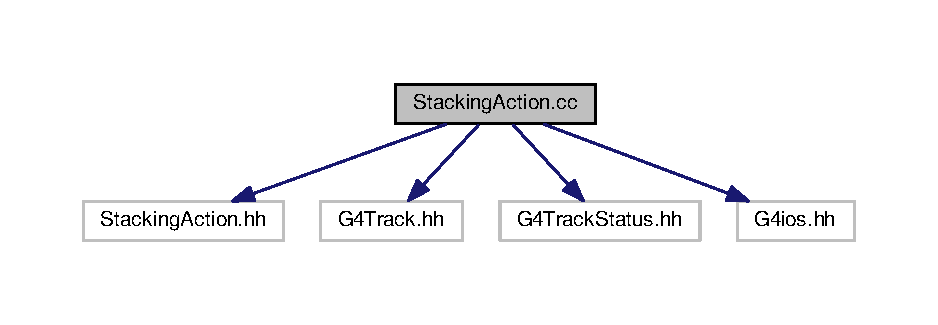
\includegraphics[width=350pt]{StackingAction_8cc__incl}
\end{center}
\end{figure}

\hypertarget{TrackingAction_8cc}{}\section{Tracking\+Action.\+cc File Reference}
\label{TrackingAction_8cc}\index{Tracking\+Action.\+cc@{Tracking\+Action.\+cc}}
{\ttfamily \#include \char`\"{}Tracking\+Action.\+hh\char`\"{}}\\*
{\ttfamily \#include \char`\"{}G4\+Track.\+hh\char`\"{}}\\*
{\ttfamily \#include \char`\"{}G4\+Positron.\+hh\char`\"{}}\\*
{\ttfamily \#include \char`\"{}G4ios.\+hh\char`\"{}}\\*
Include dependency graph for Tracking\+Action.\+cc\+:
\nopagebreak
\begin{figure}[H]
\begin{center}
\leavevmode
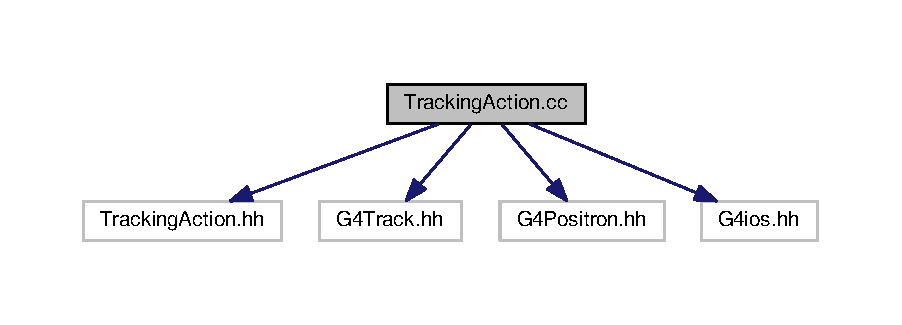
\includegraphics[width=350pt]{TrackingAction_8cc__incl}
\end{center}
\end{figure}

%--- End generated contents ---

% Index
\backmatter
\newpage
\phantomsection
\clearemptydoublepage
\addcontentsline{toc}{chapter}{Index}
\printindex

\end{document}
